\documentclass[twoside]{book}

% Packages required by doxygen
\usepackage{fixltx2e}
\usepackage{calc}
\usepackage{doxygen}
\usepackage[export]{adjustbox} % also loads graphicx
\usepackage{graphicx}
\usepackage[utf8]{inputenc}
\usepackage{makeidx}
\usepackage{multicol}
\usepackage{multirow}
\PassOptionsToPackage{warn}{textcomp}
\usepackage{textcomp}
\usepackage[nointegrals]{wasysym}
\usepackage[table]{xcolor}

% Font selection
\usepackage[T1]{fontenc}
\usepackage[scaled=.90]{helvet}
\usepackage{courier}
\usepackage{amssymb}
\usepackage{sectsty}
\renewcommand{\familydefault}{\sfdefault}
\allsectionsfont{%
  \fontseries{bc}\selectfont%
  \color{darkgray}%
}
\renewcommand{\DoxyLabelFont}{%
  \fontseries{bc}\selectfont%
  \color{darkgray}%
}
\newcommand{\+}{\discretionary{\mbox{\scriptsize$\hookleftarrow$}}{}{}}

% Page & text layout
\usepackage{geometry}
\geometry{%
  a4paper,%
  top=2.5cm,%
  bottom=2.5cm,%
  left=2.5cm,%
  right=2.5cm%
}
\tolerance=750
\hfuzz=15pt
\hbadness=750
\setlength{\emergencystretch}{15pt}
\setlength{\parindent}{0cm}
\setlength{\parskip}{0.2cm}
\makeatletter
\renewcommand{\paragraph}{%
  \@startsection{paragraph}{4}{0ex}{-1.0ex}{1.0ex}{%
    \normalfont\normalsize\bfseries\SS@parafont%
  }%
}
\renewcommand{\subparagraph}{%
  \@startsection{subparagraph}{5}{0ex}{-1.0ex}{1.0ex}{%
    \normalfont\normalsize\bfseries\SS@subparafont%
  }%
}
\makeatother

% Headers & footers
\usepackage{fancyhdr}
\pagestyle{fancyplain}
\fancyhead[LE]{\fancyplain{}{\bfseries\thepage}}
\fancyhead[CE]{\fancyplain{}{}}
\fancyhead[RE]{\fancyplain{}{\bfseries\leftmark}}
\fancyhead[LO]{\fancyplain{}{\bfseries\rightmark}}
\fancyhead[CO]{\fancyplain{}{}}
\fancyhead[RO]{\fancyplain{}{\bfseries\thepage}}
\fancyfoot[LE]{\fancyplain{}{}}
\fancyfoot[CE]{\fancyplain{}{}}
\fancyfoot[RE]{\fancyplain{}{\bfseries\scriptsize Generated on Mon Oct 5 2015 17\+:13\+:16 for C\+P\+U-\/\+O\+S Simulator by Doxygen }}
\fancyfoot[LO]{\fancyplain{}{\bfseries\scriptsize Generated on Mon Oct 5 2015 17\+:13\+:16 for C\+P\+U-\/\+O\+S Simulator by Doxygen }}
\fancyfoot[CO]{\fancyplain{}{}}
\fancyfoot[RO]{\fancyplain{}{}}
\renewcommand{\footrulewidth}{0.4pt}
\renewcommand{\chaptermark}[1]{%
  \markboth{#1}{}%
}
\renewcommand{\sectionmark}[1]{%
  \markright{\thesection\ #1}%
}

% Indices & bibliography
\usepackage{natbib}
\usepackage[titles]{tocloft}
\setcounter{tocdepth}{3}
\setcounter{secnumdepth}{5}
\makeindex

% Hyperlinks (required, but should be loaded last)
\usepackage{ifpdf}
\ifpdf
  \usepackage[pdftex,pagebackref=true]{hyperref}
\else
  \usepackage[ps2pdf,pagebackref=true]{hyperref}
\fi
\hypersetup{%
  colorlinks=true,%
  linkcolor=blue,%
  citecolor=blue,%
  unicode%
}

% Custom commands
\newcommand{\clearemptydoublepage}{%
  \newpage{\pagestyle{empty}\cleardoublepage}%
}


%===== C O N T E N T S =====

\begin{document}

% Titlepage & ToC
\hypersetup{pageanchor=false,
             bookmarks=true,
             bookmarksnumbered=true,
             pdfencoding=unicode
            }
\pagenumbering{roman}
\begin{titlepage}
\vspace*{7cm}
\begin{center}%
{\Large C\+P\+U-\/\+O\+S Simulator }\\
\vspace*{1cm}
{\large Generated by Doxygen 1.8.10}\\
\vspace*{0.5cm}
{\small Mon Oct 5 2015 17:13:16}\\
\end{center}
\end{titlepage}
\clearemptydoublepage
\tableofcontents
\clearemptydoublepage
\pagenumbering{arabic}
\hypersetup{pageanchor=true}

%--- Begin generated contents ---
\chapter{Namespace Index}
\section{Packages}
Here are the packages with brief descriptions (if available)\+:\begin{DoxyCompactList}
\item\contentsline{section}{\hyperlink{namespace_c_p_u___o_s___simulator}{C\+P\+U\+\_\+\+O\+S\+\_\+\+Simulator} }{\pageref{namespace_c_p_u___o_s___simulator}}{}
\item\contentsline{section}{\hyperlink{namespace_c_p_u___o_s___simulator_1_1_annotations}{C\+P\+U\+\_\+\+O\+S\+\_\+\+Simulator.\+Annotations} }{\pageref{namespace_c_p_u___o_s___simulator_1_1_annotations}}{}
\item\contentsline{section}{\hyperlink{namespace_c_p_u___o_s___simulator_1_1_compiler}{C\+P\+U\+\_\+\+O\+S\+\_\+\+Simulator.\+Compiler} }{\pageref{namespace_c_p_u___o_s___simulator_1_1_compiler}}{}
\item\contentsline{section}{\hyperlink{namespace_c_p_u___o_s___simulator_1_1_compiler_1_1_backend}{C\+P\+U\+\_\+\+O\+S\+\_\+\+Simulator.\+Compiler.\+Backend} }{\pageref{namespace_c_p_u___o_s___simulator_1_1_compiler_1_1_backend}}{}
\item\contentsline{section}{\hyperlink{namespace_c_p_u___o_s___simulator_1_1_compiler_1_1_frontend}{C\+P\+U\+\_\+\+O\+S\+\_\+\+Simulator.\+Compiler.\+Frontend} }{\pageref{namespace_c_p_u___o_s___simulator_1_1_compiler_1_1_frontend}}{}
\item\contentsline{section}{\hyperlink{namespace_c_p_u___o_s___simulator_1_1_compiler_1_1_frontend_1_1_symbols}{C\+P\+U\+\_\+\+O\+S\+\_\+\+Simulator.\+Compiler.\+Frontend.\+Symbols} }{\pageref{namespace_c_p_u___o_s___simulator_1_1_compiler_1_1_frontend_1_1_symbols}}{}
\item\contentsline{section}{\hyperlink{namespace_c_p_u___o_s___simulator_1_1_compiler_1_1_frontend_1_1_syntax_tree}{C\+P\+U\+\_\+\+O\+S\+\_\+\+Simulator.\+Compiler.\+Frontend.\+Syntax\+Tree} }{\pageref{namespace_c_p_u___o_s___simulator_1_1_compiler_1_1_frontend_1_1_syntax_tree}}{}
\item\contentsline{section}{\hyperlink{namespace_c_p_u___o_s___simulator_1_1_compiler_1_1_frontend_1_1_tokens}{C\+P\+U\+\_\+\+O\+S\+\_\+\+Simulator.\+Compiler.\+Frontend.\+Tokens} }{\pageref{namespace_c_p_u___o_s___simulator_1_1_compiler_1_1_frontend_1_1_tokens}}{}
\item\contentsline{section}{\hyperlink{namespace_c_p_u___o_s___simulator_1_1_compiler_tester}{C\+P\+U\+\_\+\+O\+S\+\_\+\+Simulator.\+Compiler\+Tester} }{\pageref{namespace_c_p_u___o_s___simulator_1_1_compiler_tester}}{}
\item\contentsline{section}{\hyperlink{namespace_c_p_u___o_s___simulator_1_1_compiler_tester_1_1_properties}{C\+P\+U\+\_\+\+O\+S\+\_\+\+Simulator.\+Compiler\+Tester.\+Properties} }{\pageref{namespace_c_p_u___o_s___simulator_1_1_compiler_tester_1_1_properties}}{}
\item\contentsline{section}{\hyperlink{namespace_c_p_u___o_s___simulator_1_1_console}{C\+P\+U\+\_\+\+O\+S\+\_\+\+Simulator.\+Console} }{\pageref{namespace_c_p_u___o_s___simulator_1_1_console}}{}
\item\contentsline{section}{\hyperlink{namespace_c_p_u___o_s___simulator_1_1_console_1_1_tests}{C\+P\+U\+\_\+\+O\+S\+\_\+\+Simulator.\+Console.\+Tests} }{\pageref{namespace_c_p_u___o_s___simulator_1_1_console_1_1_tests}}{}
\item\contentsline{section}{\hyperlink{namespace_c_p_u___o_s___simulator_1_1_controls}{C\+P\+U\+\_\+\+O\+S\+\_\+\+Simulator.\+Controls} }{\pageref{namespace_c_p_u___o_s___simulator_1_1_controls}}{}
\item\contentsline{section}{\hyperlink{namespace_c_p_u___o_s___simulator_1_1_controls_1_1_graphs}{C\+P\+U\+\_\+\+O\+S\+\_\+\+Simulator.\+Controls.\+Graphs} }{\pageref{namespace_c_p_u___o_s___simulator_1_1_controls_1_1_graphs}}{}
\item\contentsline{section}{\hyperlink{namespace_c_p_u___o_s___simulator_1_1_controls_1_1_graphs_1_1_view_models}{C\+P\+U\+\_\+\+O\+S\+\_\+\+Simulator.\+Controls.\+Graphs.\+View\+Models} }{\pageref{namespace_c_p_u___o_s___simulator_1_1_controls_1_1_graphs_1_1_view_models}}{}
\item\contentsline{section}{\hyperlink{namespace_c_p_u___o_s___simulator_1_1_controls_1_1_resource___controls}{C\+P\+U\+\_\+\+O\+S\+\_\+\+Simulator.\+Controls.\+Resource\+\_\+\+Controls} }{\pageref{namespace_c_p_u___o_s___simulator_1_1_controls_1_1_resource___controls}}{}
\item\contentsline{section}{\hyperlink{namespace_c_p_u___o_s___simulator_1_1_controls_1_1_resource___controls_1_1_shapes}{C\+P\+U\+\_\+\+O\+S\+\_\+\+Simulator.\+Controls.\+Resource\+\_\+\+Controls.\+Shapes} }{\pageref{namespace_c_p_u___o_s___simulator_1_1_controls_1_1_resource___controls_1_1_shapes}}{}
\item\contentsline{section}{\hyperlink{namespace_c_p_u___o_s___simulator_1_1_c_p_u}{C\+P\+U\+\_\+\+O\+S\+\_\+\+Simulator.\+C\+P\+U} }{\pageref{namespace_c_p_u___o_s___simulator_1_1_c_p_u}}{}
\item\contentsline{section}{\hyperlink{namespace_c_p_u___o_s___simulator_1_1_c_p_u_1_1_interrupts}{C\+P\+U\+\_\+\+O\+S\+\_\+\+Simulator.\+C\+P\+U.\+Interrupts} }{\pageref{namespace_c_p_u___o_s___simulator_1_1_c_p_u_1_1_interrupts}}{}
\item\contentsline{section}{\hyperlink{namespace_c_p_u___o_s___simulator_1_1_c_p_u_1_1_tests}{C\+P\+U\+\_\+\+O\+S\+\_\+\+Simulator.\+C\+P\+U.\+Tests} }{\pageref{namespace_c_p_u___o_s___simulator_1_1_c_p_u_1_1_tests}}{}
\item\contentsline{section}{\hyperlink{namespace_c_p_u___o_s___simulator_1_1_memory}{C\+P\+U\+\_\+\+O\+S\+\_\+\+Simulator.\+Memory} }{\pageref{namespace_c_p_u___o_s___simulator_1_1_memory}}{}
\item\contentsline{section}{\hyperlink{namespace_c_p_u___o_s___simulator_1_1_memory_1_1_tests}{C\+P\+U\+\_\+\+O\+S\+\_\+\+Simulator.\+Memory.\+Tests} }{\pageref{namespace_c_p_u___o_s___simulator_1_1_memory_1_1_tests}}{}
\item\contentsline{section}{\hyperlink{namespace_c_p_u___o_s___simulator_1_1_operating___system}{C\+P\+U\+\_\+\+O\+S\+\_\+\+Simulator.\+Operating\+\_\+\+System} }{\pageref{namespace_c_p_u___o_s___simulator_1_1_operating___system}}{}
\item\contentsline{section}{\hyperlink{namespace_c_p_u___o_s___simulator_1_1_operating___system_1_1_threading}{C\+P\+U\+\_\+\+O\+S\+\_\+\+Simulator.\+Operating\+\_\+\+System.\+Threading} }{\pageref{namespace_c_p_u___o_s___simulator_1_1_operating___system_1_1_threading}}{}
\item\contentsline{section}{\hyperlink{namespace_c_p_u___o_s___simulator_1_1_properties}{C\+P\+U\+\_\+\+O\+S\+\_\+\+Simulator.\+Properties} }{\pageref{namespace_c_p_u___o_s___simulator_1_1_properties}}{}
\item\contentsline{section}{\hyperlink{namespace_c_p_u___o_s___simulator_1_1_save___file___editor}{C\+P\+U\+\_\+\+O\+S\+\_\+\+Simulator.\+Save\+\_\+\+File\+\_\+\+Editor} }{\pageref{namespace_c_p_u___o_s___simulator_1_1_save___file___editor}}{}
\item\contentsline{section}{\hyperlink{namespace_c_p_u___o_s___simulator_1_1_save___file___editor_1_1_properties}{C\+P\+U\+\_\+\+O\+S\+\_\+\+Simulator.\+Save\+\_\+\+File\+\_\+\+Editor.\+Properties} }{\pageref{namespace_c_p_u___o_s___simulator_1_1_save___file___editor_1_1_properties}}{}
\item\contentsline{section}{\hyperlink{namespace_c_p_u___o_s___simulator_1_1_tests}{C\+P\+U\+\_\+\+O\+S\+\_\+\+Simulator.\+Tests} }{\pageref{namespace_c_p_u___o_s___simulator_1_1_tests}}{}
\item\contentsline{section}{\hyperlink{namespace_c_p_u___o_s___simulator_1_1_window_bridge}{C\+P\+U\+\_\+\+O\+S\+\_\+\+Simulator.\+Window\+Bridge} }{\pageref{namespace_c_p_u___o_s___simulator_1_1_window_bridge}}{}
\item\contentsline{section}{\hyperlink{namespace_save_file_editor}{Save\+File\+Editor} }{\pageref{namespace_save_file_editor}}{}
\item\contentsline{section}{\hyperlink{namespace_xaml_generated_namespace}{Xaml\+Generated\+Namespace} }{\pageref{namespace_xaml_generated_namespace}}{}
\end{DoxyCompactList}

\chapter{Hierarchical Index}
\section{Class Hierarchy}
This inheritance list is sorted roughly, but not completely, alphabetically\+:\begin{DoxyCompactList}
\item \contentsline{section}{Xaml\+Static\+Helper\+Namespace.\+\_\+\+Xaml\+Static\+Helper}{\pageref{class_xaml_static_helper_namespace_1_1___xaml_static_helper}}{}
\item Activity\begin{DoxyCompactList}
\item \contentsline{section}{C\+P\+U\+\_\+\+O\+S\+\_\+\+Simulator.\+C\+P\+U.\+Activity1}{\pageref{class_c_p_u___o_s___simulator_1_1_c_p_u_1_1_activity1}}{}
\end{DoxyCompactList}
\item Application\begin{DoxyCompactList}
\item \contentsline{section}{C\+P\+U\+\_\+\+O\+S\+\_\+\+Simulator.\+App}{\pageref{class_c_p_u___o_s___simulator_1_1_app}}{}
\item \contentsline{section}{C\+P\+U\+\_\+\+O\+S\+\_\+\+Simulator.\+App}{\pageref{class_c_p_u___o_s___simulator_1_1_app}}{}
\item \contentsline{section}{C\+P\+U\+\_\+\+O\+S\+\_\+\+Simulator.\+App}{\pageref{class_c_p_u___o_s___simulator_1_1_app}}{}
\item \contentsline{section}{C\+P\+U\+\_\+\+O\+S\+\_\+\+Simulator.\+App}{\pageref{class_c_p_u___o_s___simulator_1_1_app}}{}
\item \contentsline{section}{C\+P\+U\+\_\+\+O\+S\+\_\+\+Simulator.\+App}{\pageref{class_c_p_u___o_s___simulator_1_1_app}}{}
\end{DoxyCompactList}
\item Application\+Settings\+Base\begin{DoxyCompactList}
\item \contentsline{section}{C\+P\+U\+\_\+\+O\+S\+\_\+\+Simulator.\+Properties.\+Settings}{\pageref{class_c_p_u___o_s___simulator_1_1_properties_1_1_settings}}{}
\end{DoxyCompactList}
\item Attribute\begin{DoxyCompactList}
\item \contentsline{section}{C\+P\+U\+\_\+\+O\+S\+\_\+\+Simulator.\+C\+P\+U.\+Number\+Of\+Operands\+Attribute}{\pageref{class_c_p_u___o_s___simulator_1_1_c_p_u_1_1_number_of_operands_attribute}}{}
\end{DoxyCompactList}
\item \contentsline{section}{C\+P\+U\+\_\+\+O\+S\+\_\+\+Simulator.\+C\+P\+U.\+Execution\+Unit}{\pageref{class_c_p_u___o_s___simulator_1_1_c_p_u_1_1_execution_unit}}{}
\item \contentsline{section}{C\+P\+U\+\_\+\+O\+S\+\_\+\+Simulator.\+C\+P\+U.\+Extentions}{\pageref{class_c_p_u___o_s___simulator_1_1_c_p_u_1_1_extentions}}{}
\item \contentsline{section}{C\+P\+U\+\_\+\+O\+S\+\_\+\+Simulator.\+C\+P\+U.\+I\+Attribute$<$ T $>$}{\pageref{interface_c_p_u___o_s___simulator_1_1_c_p_u_1_1_i_attribute}}{}
\item \contentsline{section}{C\+P\+U\+\_\+\+O\+S\+\_\+\+Simulator.\+C\+P\+U.\+I\+Attribute$<$ int $>$}{\pageref{interface_c_p_u___o_s___simulator_1_1_c_p_u_1_1_i_attribute}}{}
\begin{DoxyCompactList}
\item \contentsline{section}{C\+P\+U\+\_\+\+O\+S\+\_\+\+Simulator.\+C\+P\+U.\+Number\+Of\+Operands\+Attribute}{\pageref{class_c_p_u___o_s___simulator_1_1_c_p_u_1_1_number_of_operands_attribute}}{}
\end{DoxyCompactList}
\item I\+Component\+Connector\begin{DoxyCompactList}
\item \contentsline{section}{C\+P\+U\+\_\+\+O\+S\+\_\+\+Simulator.\+Instructions\+Window}{\pageref{class_c_p_u___o_s___simulator_1_1_instructions_window}}{}
\item \contentsline{section}{C\+P\+U\+\_\+\+O\+S\+\_\+\+Simulator.\+Instructions\+Window}{\pageref{class_c_p_u___o_s___simulator_1_1_instructions_window}}{}
\item \contentsline{section}{C\+P\+U\+\_\+\+O\+S\+\_\+\+Simulator.\+Instructions\+Window}{\pageref{class_c_p_u___o_s___simulator_1_1_instructions_window}}{}
\item \contentsline{section}{C\+P\+U\+\_\+\+O\+S\+\_\+\+Simulator.\+Instructions\+Window}{\pageref{class_c_p_u___o_s___simulator_1_1_instructions_window}}{}
\item \contentsline{section}{C\+P\+U\+\_\+\+O\+S\+\_\+\+Simulator.\+Main\+Window}{\pageref{class_c_p_u___o_s___simulator_1_1_main_window}}{}
\item \contentsline{section}{C\+P\+U\+\_\+\+O\+S\+\_\+\+Simulator.\+Main\+Window}{\pageref{class_c_p_u___o_s___simulator_1_1_main_window}}{}
\item \contentsline{section}{C\+P\+U\+\_\+\+O\+S\+\_\+\+Simulator.\+Main\+Window}{\pageref{class_c_p_u___o_s___simulator_1_1_main_window}}{}
\item \contentsline{section}{C\+P\+U\+\_\+\+O\+S\+\_\+\+Simulator.\+Main\+Window}{\pageref{class_c_p_u___o_s___simulator_1_1_main_window}}{}
\end{DoxyCompactList}
\item \contentsline{section}{C\+P\+U\+\_\+\+O\+S\+\_\+\+Simulator.\+C\+P\+U.\+Instruction}{\pageref{class_c_p_u___o_s___simulator_1_1_c_p_u_1_1_instruction}}{}
\item I\+Support\+Initialize\begin{DoxyCompactList}
\item \contentsline{section}{C\+P\+U\+\_\+\+O\+S\+\_\+\+Simulator.\+C\+P\+U.\+Activity1}{\pageref{class_c_p_u___o_s___simulator_1_1_c_p_u_1_1_activity1}}{}
\end{DoxyCompactList}
\item \contentsline{section}{C\+P\+U\+\_\+\+O\+S\+\_\+\+Simulator.\+Memory.\+Memory\+Page}{\pageref{class_c_p_u___o_s___simulator_1_1_memory_1_1_memory_page}}{}
\item \contentsline{section}{C\+P\+U\+\_\+\+O\+S\+\_\+\+Simulator.\+C\+P\+U.\+Operand}{\pageref{class_c_p_u___o_s___simulator_1_1_c_p_u_1_1_operand}}{}
\item \contentsline{section}{C\+P\+U\+\_\+\+O\+S\+\_\+\+Simulator.\+C\+P\+U.\+Program\+Stack}{\pageref{class_c_p_u___o_s___simulator_1_1_c_p_u_1_1_program_stack}}{}
\item \contentsline{section}{C\+P\+U\+\_\+\+O\+S\+\_\+\+Simulator.\+C\+P\+U.\+Register}{\pageref{class_c_p_u___o_s___simulator_1_1_c_p_u_1_1_register}}{}
\begin{DoxyCompactList}
\item \contentsline{section}{C\+P\+U\+\_\+\+O\+S\+\_\+\+Simulator.\+C\+P\+U.\+Special\+Register}{\pageref{class_c_p_u___o_s___simulator_1_1_c_p_u_1_1_special_register}}{}
\end{DoxyCompactList}
\item \contentsline{section}{C\+P\+U\+\_\+\+O\+S\+\_\+\+Simulator.\+Properties.\+Resources}{\pageref{class_c_p_u___o_s___simulator_1_1_properties_1_1_resources}}{}
\item \contentsline{section}{C\+P\+U\+\_\+\+O\+S\+\_\+\+Simulator.\+C\+P\+U.\+Simulator\+Program}{\pageref{class_c_p_u___o_s___simulator_1_1_c_p_u_1_1_simulator_program}}{}
\item \contentsline{section}{C\+P\+U\+\_\+\+O\+S\+\_\+\+Simulator.\+C\+P\+U.\+Stack\+Item}{\pageref{class_c_p_u___o_s___simulator_1_1_c_p_u_1_1_stack_item}}{}
\item \contentsline{section}{C\+P\+U\+\_\+\+O\+S\+\_\+\+Simulator.\+C\+P\+U.\+Status\+Flags}{\pageref{class_c_p_u___o_s___simulator_1_1_c_p_u_1_1_status_flags}}{}
\item Window\begin{DoxyCompactList}
\item \contentsline{section}{C\+P\+U\+\_\+\+O\+S\+\_\+\+Simulator.\+Instructions\+Window}{\pageref{class_c_p_u___o_s___simulator_1_1_instructions_window}}{}
\item \contentsline{section}{C\+P\+U\+\_\+\+O\+S\+\_\+\+Simulator.\+Instructions\+Window}{\pageref{class_c_p_u___o_s___simulator_1_1_instructions_window}}{}
\item \contentsline{section}{C\+P\+U\+\_\+\+O\+S\+\_\+\+Simulator.\+Instructions\+Window}{\pageref{class_c_p_u___o_s___simulator_1_1_instructions_window}}{}
\item \contentsline{section}{C\+P\+U\+\_\+\+O\+S\+\_\+\+Simulator.\+Instructions\+Window}{\pageref{class_c_p_u___o_s___simulator_1_1_instructions_window}}{}
\item \contentsline{section}{C\+P\+U\+\_\+\+O\+S\+\_\+\+Simulator.\+Instructions\+Window}{\pageref{class_c_p_u___o_s___simulator_1_1_instructions_window}}{}
\item \contentsline{section}{C\+P\+U\+\_\+\+O\+S\+\_\+\+Simulator.\+Main\+Window}{\pageref{class_c_p_u___o_s___simulator_1_1_main_window}}{}
\item \contentsline{section}{C\+P\+U\+\_\+\+O\+S\+\_\+\+Simulator.\+Main\+Window}{\pageref{class_c_p_u___o_s___simulator_1_1_main_window}}{}
\item \contentsline{section}{C\+P\+U\+\_\+\+O\+S\+\_\+\+Simulator.\+Main\+Window}{\pageref{class_c_p_u___o_s___simulator_1_1_main_window}}{}
\item \contentsline{section}{C\+P\+U\+\_\+\+O\+S\+\_\+\+Simulator.\+Main\+Window}{\pageref{class_c_p_u___o_s___simulator_1_1_main_window}}{}
\item \contentsline{section}{C\+P\+U\+\_\+\+O\+S\+\_\+\+Simulator.\+Main\+Window}{\pageref{class_c_p_u___o_s___simulator_1_1_main_window}}{}
\end{DoxyCompactList}
\item \contentsline{section}{C\+P\+U\+\_\+\+O\+S\+\_\+\+Simulator.\+Window\+Bridge.\+Window\+Instances}{\pageref{class_c_p_u___o_s___simulator_1_1_window_bridge_1_1_window_instances}}{}
\end{DoxyCompactList}

\chapter{Class Index}
\section{Class List}
Here are the classes, structs, unions and interfaces with brief descriptions\+:\begin{DoxyCompactList}
\item\contentsline{section}{\hyperlink{class_c_p_u___o_s___simulator_1_1_app}{C\+P\+U\+\_\+\+O\+S\+\_\+\+Simulator.\+App} \\*Interaction logic for App.\+xaml }{\pageref{class_c_p_u___o_s___simulator_1_1_app}}{}
\item\contentsline{section}{\hyperlink{class_c_p_u___o_s___simulator_1_1_colour_picker_window}{C\+P\+U\+\_\+\+O\+S\+\_\+\+Simulator.\+Colour\+Picker\+Window} \\*Interaction logic for Colour\+Picker\+Window.\+xaml }{\pageref{class_c_p_u___o_s___simulator_1_1_colour_picker_window}}{}
\item\contentsline{section}{\hyperlink{class_c_p_u___o_s___simulator_1_1_c_p_u_1_1_compiled_program}{C\+P\+U\+\_\+\+O\+S\+\_\+\+Simulator.\+C\+P\+U.\+Compiled\+Program} \\*This class represents a program after it has been compiled }{\pageref{class_c_p_u___o_s___simulator_1_1_c_p_u_1_1_compiled_program}}{}
\item\contentsline{section}{\hyperlink{class_c_p_u___o_s___simulator_1_1_compiler_1_1_compiler_frontend}{C\+P\+U\+\_\+\+O\+S\+\_\+\+Simulator.\+Compiler.\+Compiler\+Frontend} \\*This class represents the front end of the compiler which is responsible for compiling programs }{\pageref{class_c_p_u___o_s___simulator_1_1_compiler_1_1_compiler_frontend}}{}
\item\contentsline{section}{\hyperlink{class_c_p_u___o_s___simulator_1_1_console_1_1_console_command}{C\+P\+U\+\_\+\+O\+S\+\_\+\+Simulator.\+Console.\+Console\+Command} \\*This class represents a console command }{\pageref{class_c_p_u___o_s___simulator_1_1_console_1_1_console_command}}{}
\item\contentsline{section}{\hyperlink{class_c_p_u___o_s___simulator_1_1_console_1_1_console_input}{C\+P\+U\+\_\+\+O\+S\+\_\+\+Simulator.\+Console.\+Console\+Input} \\*This class represents an input made through the console }{\pageref{class_c_p_u___o_s___simulator_1_1_console_1_1_console_input}}{}
\item\contentsline{section}{\hyperlink{class_c_p_u___o_s___simulator_1_1_console_1_1_console_output}{C\+P\+U\+\_\+\+O\+S\+\_\+\+Simulator.\+Console.\+Console\+Output} \\*This class represents an output made through the console }{\pageref{class_c_p_u___o_s___simulator_1_1_console_1_1_console_output}}{}
\item\contentsline{section}{\hyperlink{class_c_p_u___o_s___simulator_1_1_console_window}{C\+P\+U\+\_\+\+O\+S\+\_\+\+Simulator.\+Console\+Window} \\*Interaction logic for Console\+Window.\+xaml }{\pageref{class_c_p_u___o_s___simulator_1_1_console_window}}{}
\item\contentsline{section}{\hyperlink{class_c_p_u___o_s___simulator_1_1_c_p_u_1_1_execution_unit}{C\+P\+U\+\_\+\+O\+S\+\_\+\+Simulator.\+C\+P\+U.\+Execution\+Unit} \\*This class represents the part of the \hyperlink{namespace_c_p_u___o_s___simulator_1_1_c_p_u}{C\+P\+U} which executes instructions }{\pageref{class_c_p_u___o_s___simulator_1_1_c_p_u_1_1_execution_unit}}{}
\item\contentsline{section}{\hyperlink{class_c_p_u___o_s___simulator_1_1_c_p_u_1_1_tests_1_1_execution_unit_tests}{C\+P\+U\+\_\+\+O\+S\+\_\+\+Simulator.\+C\+P\+U.\+Tests.\+Execution\+Unit\+Tests} }{\pageref{class_c_p_u___o_s___simulator_1_1_c_p_u_1_1_tests_1_1_execution_unit_tests}}{}
\item\contentsline{section}{\hyperlink{class_c_p_u___o_s___simulator_1_1_c_p_u_1_1_extentions}{C\+P\+U\+\_\+\+O\+S\+\_\+\+Simulator.\+C\+P\+U.\+Extentions} \\*This class contains extension methods for getting attributes from enum items }{\pageref{class_c_p_u___o_s___simulator_1_1_c_p_u_1_1_extentions}}{}
\item\contentsline{section}{\hyperlink{class_c_p_u___o_s___simulator_1_1_console_1_1_extentions}{C\+P\+U\+\_\+\+O\+S\+\_\+\+Simulator.\+Console.\+Extentions} \\*This class contains extension methods for getting attributes from enum items }{\pageref{class_c_p_u___o_s___simulator_1_1_console_1_1_extentions}}{}
\item\contentsline{section}{\hyperlink{interface_c_p_u___o_s___simulator_1_1_console_1_1_i_attribute}{C\+P\+U\+\_\+\+O\+S\+\_\+\+Simulator.\+Console.\+I\+Attribute$<$ T $>$} \\*This interface represents a attribute with a single value }{\pageref{interface_c_p_u___o_s___simulator_1_1_console_1_1_i_attribute}}{}
\item\contentsline{section}{\hyperlink{interface_c_p_u___o_s___simulator_1_1_c_p_u_1_1_i_attribute}{C\+P\+U\+\_\+\+O\+S\+\_\+\+Simulator.\+C\+P\+U.\+I\+Attribute$<$ T $>$} \\*This interface defines a basic attribute }{\pageref{interface_c_p_u___o_s___simulator_1_1_c_p_u_1_1_i_attribute}}{}
\item\contentsline{section}{\hyperlink{class_c_p_u___o_s___simulator_1_1_c_p_u_1_1_instruction}{C\+P\+U\+\_\+\+O\+S\+\_\+\+Simulator.\+C\+P\+U.\+Instruction} \\*This class represents an instruction witch can be executed by the virtual \hyperlink{namespace_c_p_u___o_s___simulator_1_1_c_p_u}{C\+P\+U} }{\pageref{class_c_p_u___o_s___simulator_1_1_c_p_u_1_1_instruction}}{}
\item\contentsline{section}{\hyperlink{class_c_p_u___o_s___simulator_1_1_compiler_1_1_instruction_segment}{C\+P\+U\+\_\+\+O\+S\+\_\+\+Simulator.\+Compiler.\+Instruction\+Segment} \\*this class represents a segment of an instruction i.\+e the opcode or an operand }{\pageref{class_c_p_u___o_s___simulator_1_1_compiler_1_1_instruction_segment}}{}
\item\contentsline{section}{\hyperlink{class_c_p_u___o_s___simulator_1_1_instructions_window}{C\+P\+U\+\_\+\+O\+S\+\_\+\+Simulator.\+Instructions\+Window} \\*Interaction logic for Instructions\+Window.\+xaml }{\pageref{class_c_p_u___o_s___simulator_1_1_instructions_window}}{}
\item\contentsline{section}{\hyperlink{class_c_p_u___o_s___simulator_1_1_tests_1_1_instructions_window_tests}{C\+P\+U\+\_\+\+O\+S\+\_\+\+Simulator.\+Tests.\+Instructions\+Window\+Tests} }{\pageref{class_c_p_u___o_s___simulator_1_1_tests_1_1_instructions_window_tests}}{}
\item\contentsline{section}{\hyperlink{class_c_p_u___o_s___simulator_1_1_c_p_u_1_1_tests_1_1_instruction_tests}{C\+P\+U\+\_\+\+O\+S\+\_\+\+Simulator.\+C\+P\+U.\+Tests.\+Instruction\+Tests} }{\pageref{class_c_p_u___o_s___simulator_1_1_c_p_u_1_1_tests_1_1_instruction_tests}}{}
\item\contentsline{section}{\hyperlink{interface_c_p_u___o_s___simulator_1_1_memory_1_1_i_swappable}{C\+P\+U\+\_\+\+O\+S\+\_\+\+Simulator.\+Memory.\+I\+Swappable} }{\pageref{interface_c_p_u___o_s___simulator_1_1_memory_1_1_i_swappable}}{}
\item\contentsline{section}{\hyperlink{class_c_p_u___o_s___simulator_1_1_main_window}{C\+P\+U\+\_\+\+O\+S\+\_\+\+Simulator.\+Main\+Window} \\*Interaction logic for Main\+Window.\+xaml }{\pageref{class_c_p_u___o_s___simulator_1_1_main_window}}{}
\item\contentsline{section}{\hyperlink{class_c_p_u___o_s___simulator_1_1_tests_1_1_main_window_tests}{C\+P\+U\+\_\+\+O\+S\+\_\+\+Simulator.\+Tests.\+Main\+Window\+Tests} }{\pageref{class_c_p_u___o_s___simulator_1_1_tests_1_1_main_window_tests}}{}
\item\contentsline{section}{\hyperlink{class_c_p_u___o_s___simulator_1_1_memory_1_1_memory_page}{C\+P\+U\+\_\+\+O\+S\+\_\+\+Simulator.\+Memory.\+Memory\+Page} \\*This class represents a page of data within memory }{\pageref{class_c_p_u___o_s___simulator_1_1_memory_1_1_memory_page}}{}
\item\contentsline{section}{\hyperlink{class_c_p_u___o_s___simulator_1_1_memory_1_1_tests_1_1_memory_page_tests}{C\+P\+U\+\_\+\+O\+S\+\_\+\+Simulator.\+Memory.\+Tests.\+Memory\+Page\+Tests} }{\pageref{class_c_p_u___o_s___simulator_1_1_memory_1_1_tests_1_1_memory_page_tests}}{}
\item\contentsline{section}{\hyperlink{class_c_p_u___o_s___simulator_1_1_memory_1_1_memory_segment}{C\+P\+U\+\_\+\+O\+S\+\_\+\+Simulator.\+Memory.\+Memory\+Segment} \\*This class represents a 8 byte segment of a memory page }{\pageref{class_c_p_u___o_s___simulator_1_1_memory_1_1_memory_segment}}{}
\item\contentsline{section}{\hyperlink{class_c_p_u___o_s___simulator_1_1_memory_1_1_tests_1_1_memory_segment_tests}{C\+P\+U\+\_\+\+O\+S\+\_\+\+Simulator.\+Memory.\+Tests.\+Memory\+Segment\+Tests} }{\pageref{class_c_p_u___o_s___simulator_1_1_memory_1_1_tests_1_1_memory_segment_tests}}{}
\item\contentsline{section}{\hyperlink{class_c_p_u___o_s___simulator_1_1_memory_window}{C\+P\+U\+\_\+\+O\+S\+\_\+\+Simulator.\+Memory\+Window} \\*Interaction logic for Memory\+Window.\+xaml }{\pageref{class_c_p_u___o_s___simulator_1_1_memory_window}}{}
\item\contentsline{section}{\hyperlink{class_c_p_u___o_s___simulator_1_1_c_p_u_1_1_number_of_operands_attribute}{C\+P\+U\+\_\+\+O\+S\+\_\+\+Simulator.\+C\+P\+U.\+Number\+Of\+Operands\+Attribute} \\*This class represents the Number\+Of\+Operands attribute }{\pageref{class_c_p_u___o_s___simulator_1_1_c_p_u_1_1_number_of_operands_attribute}}{}
\item\contentsline{section}{\hyperlink{class_c_p_u___o_s___simulator_1_1_console_1_1_number_of_parameters_attribute}{C\+P\+U\+\_\+\+O\+S\+\_\+\+Simulator.\+Console.\+Number\+Of\+Parameters\+Attribute} \\*This class represents an attribute placed on console commands to indicate how many parameters they take }{\pageref{class_c_p_u___o_s___simulator_1_1_console_1_1_number_of_parameters_attribute}}{}
\item\contentsline{section}{\hyperlink{class_c_p_u___o_s___simulator_1_1_c_p_u_1_1_operand}{C\+P\+U\+\_\+\+O\+S\+\_\+\+Simulator.\+C\+P\+U.\+Operand} \\*This class represents an operand which can be passed to an instruction }{\pageref{class_c_p_u___o_s___simulator_1_1_c_p_u_1_1_operand}}{}
\item\contentsline{section}{\hyperlink{class_c_p_u___o_s___simulator_1_1_c_p_u_1_1_tests_1_1_operand_tests}{C\+P\+U\+\_\+\+O\+S\+\_\+\+Simulator.\+C\+P\+U.\+Tests.\+Operand\+Tests} }{\pageref{class_c_p_u___o_s___simulator_1_1_c_p_u_1_1_tests_1_1_operand_tests}}{}
\item\contentsline{section}{\hyperlink{class_c_p_u___o_s___simulator_1_1_memory_1_1_page_table}{C\+P\+U\+\_\+\+O\+S\+\_\+\+Simulator.\+Memory.\+Page\+Table} \\*This class represents a page table where information about the loctions of memory pages are kept }{\pageref{class_c_p_u___o_s___simulator_1_1_memory_1_1_page_table}}{}
\item\contentsline{section}{\hyperlink{class_c_p_u___o_s___simulator_1_1_memory_1_1_page_table_entry}{C\+P\+U\+\_\+\+O\+S\+\_\+\+Simulator.\+Memory.\+Page\+Table\+Entry} \\*This class represents an entry within a page table }{\pageref{class_c_p_u___o_s___simulator_1_1_memory_1_1_page_table_entry}}{}
\item\contentsline{section}{\hyperlink{class_c_p_u___o_s___simulator_1_1_page_table_window}{C\+P\+U\+\_\+\+O\+S\+\_\+\+Simulator.\+Page\+Table\+Window} \\*\hyperlink{class_c_p_u___o_s___simulator_1_1_page_table_window}{Page\+Table\+Window} }{\pageref{class_c_p_u___o_s___simulator_1_1_page_table_window}}{}
\item\contentsline{section}{\hyperlink{class_c_p_u___o_s___simulator_1_1_memory_1_1_physical_memory}{C\+P\+U\+\_\+\+O\+S\+\_\+\+Simulator.\+Memory.\+Physical\+Memory} \\*This class represents physical memory (R\+A\+M) }{\pageref{class_c_p_u___o_s___simulator_1_1_memory_1_1_physical_memory}}{}
\item\contentsline{section}{\hyperlink{class_c_p_u___o_s___simulator_1_1_c_p_u_1_1_program_stack}{C\+P\+U\+\_\+\+O\+S\+\_\+\+Simulator.\+C\+P\+U.\+Program\+Stack} \\*This class represents a Last in first out (L\+I\+F\+O) stack data structure for use with simulator programs }{\pageref{class_c_p_u___o_s___simulator_1_1_c_p_u_1_1_program_stack}}{}
\item\contentsline{section}{\hyperlink{class_c_p_u___o_s___simulator_1_1_c_p_u_1_1_tests_1_1_program_stack_tests}{C\+P\+U\+\_\+\+O\+S\+\_\+\+Simulator.\+C\+P\+U.\+Tests.\+Program\+Stack\+Tests} }{\pageref{class_c_p_u___o_s___simulator_1_1_c_p_u_1_1_tests_1_1_program_stack_tests}}{}
\item\contentsline{section}{\hyperlink{class_c_p_u___o_s___simulator_1_1_c_p_u_1_1_register}{C\+P\+U\+\_\+\+O\+S\+\_\+\+Simulator.\+C\+P\+U.\+Register} \\*This class represents a \hyperlink{namespace_c_p_u___o_s___simulator_1_1_c_p_u}{C\+P\+U} register }{\pageref{class_c_p_u___o_s___simulator_1_1_c_p_u_1_1_register}}{}
\item\contentsline{section}{\hyperlink{class_c_p_u___o_s___simulator_1_1_c_p_u_1_1_tests_1_1_register_tests}{C\+P\+U\+\_\+\+O\+S\+\_\+\+Simulator.\+C\+P\+U.\+Tests.\+Register\+Tests} }{\pageref{class_c_p_u___o_s___simulator_1_1_c_p_u_1_1_tests_1_1_register_tests}}{}
\item\contentsline{section}{\hyperlink{class_c_p_u___o_s___simulator_1_1_properties_1_1_resources}{C\+P\+U\+\_\+\+O\+S\+\_\+\+Simulator.\+Properties.\+Resources} \\*A strongly-\/typed resource class, for looking up localized strings, etc. }{\pageref{class_c_p_u___o_s___simulator_1_1_properties_1_1_resources}}{}
\item\contentsline{section}{\hyperlink{class_c_p_u___o_s___simulator_1_1_properties_1_1_settings}{C\+P\+U\+\_\+\+O\+S\+\_\+\+Simulator.\+Properties.\+Settings} }{\pageref{class_c_p_u___o_s___simulator_1_1_properties_1_1_settings}}{}
\item\contentsline{section}{\hyperlink{class_c_p_u___o_s___simulator_1_1_c_p_u_1_1_simulator_program}{C\+P\+U\+\_\+\+O\+S\+\_\+\+Simulator.\+C\+P\+U.\+Simulator\+Program} \\*This class represents a program that can be run within the simulator }{\pageref{class_c_p_u___o_s___simulator_1_1_c_p_u_1_1_simulator_program}}{}
\item\contentsline{section}{\hyperlink{class_c_p_u___o_s___simulator_1_1_c_p_u_1_1_tests_1_1_simulator_program_tests}{C\+P\+U\+\_\+\+O\+S\+\_\+\+Simulator.\+C\+P\+U.\+Tests.\+Simulator\+Program\+Tests} }{\pageref{class_c_p_u___o_s___simulator_1_1_c_p_u_1_1_tests_1_1_simulator_program_tests}}{}
\item\contentsline{section}{\hyperlink{class_c_p_u___o_s___simulator_1_1_compiler_1_1_source_file}{C\+P\+U\+\_\+\+O\+S\+\_\+\+Simulator.\+Compiler.\+Source\+File} \\*This class represents a program source file to be compiled by the compiler }{\pageref{class_c_p_u___o_s___simulator_1_1_compiler_1_1_source_file}}{}
\item\contentsline{section}{\hyperlink{class_c_p_u___o_s___simulator_1_1_c_p_u_1_1_special_register}{C\+P\+U\+\_\+\+O\+S\+\_\+\+Simulator.\+C\+P\+U.\+Special\+Register} \\*This class represents a special register i.\+e a non general purpose register }{\pageref{class_c_p_u___o_s___simulator_1_1_c_p_u_1_1_special_register}}{}
\item\contentsline{section}{\hyperlink{class_c_p_u___o_s___simulator_1_1_c_p_u_1_1_tests_1_1_special_register_tests}{C\+P\+U\+\_\+\+O\+S\+\_\+\+Simulator.\+C\+P\+U.\+Tests.\+Special\+Register\+Tests} }{\pageref{class_c_p_u___o_s___simulator_1_1_c_p_u_1_1_tests_1_1_special_register_tests}}{}
\item\contentsline{section}{\hyperlink{class_c_p_u___o_s___simulator_1_1_c_p_u_1_1_stack_item}{C\+P\+U\+\_\+\+O\+S\+\_\+\+Simulator.\+C\+P\+U.\+Stack\+Item} \\*This class represents an item that is stored on the stack }{\pageref{class_c_p_u___o_s___simulator_1_1_c_p_u_1_1_stack_item}}{}
\item\contentsline{section}{\hyperlink{class_c_p_u___o_s___simulator_1_1_c_p_u_1_1_tests_1_1_stack_item_tests}{C\+P\+U\+\_\+\+O\+S\+\_\+\+Simulator.\+C\+P\+U.\+Tests.\+Stack\+Item\+Tests} }{\pageref{class_c_p_u___o_s___simulator_1_1_c_p_u_1_1_tests_1_1_stack_item_tests}}{}
\item\contentsline{section}{\hyperlink{class_c_p_u___o_s___simulator_1_1_c_p_u_1_1_status_flags}{C\+P\+U\+\_\+\+O\+S\+\_\+\+Simulator.\+C\+P\+U.\+Status\+Flags} \\*This class represents a status flag used within the \hyperlink{namespace_c_p_u___o_s___simulator_1_1_c_p_u}{C\+P\+U} to determine whether a condition has been met. }{\pageref{class_c_p_u___o_s___simulator_1_1_c_p_u_1_1_status_flags}}{}
\item\contentsline{section}{\hyperlink{class_c_p_u___o_s___simulator_1_1_c_p_u_1_1_tests_1_1_status_flags_tests}{C\+P\+U\+\_\+\+O\+S\+\_\+\+Simulator.\+C\+P\+U.\+Tests.\+Status\+Flags\+Tests} }{\pageref{class_c_p_u___o_s___simulator_1_1_c_p_u_1_1_tests_1_1_status_flags_tests}}{}
\item\contentsline{section}{\hyperlink{class_c_p_u___o_s___simulator_1_1_memory_1_1_swap_space}{C\+P\+U\+\_\+\+O\+S\+\_\+\+Simulator.\+Memory.\+Swap\+Space} \\*This class represents swap space where swapped outmemory pages are moved to }{\pageref{class_c_p_u___o_s___simulator_1_1_memory_1_1_swap_space}}{}
\item\contentsline{section}{\hyperlink{class_c_p_u___o_s___simulator_1_1_window_bridge_1_1_window_instances}{C\+P\+U\+\_\+\+O\+S\+\_\+\+Simulator.\+Window\+Bridge.\+Window\+Instances} \\*This class represents all of the active window instances }{\pageref{class_c_p_u___o_s___simulator_1_1_window_bridge_1_1_window_instances}}{}
\end{DoxyCompactList}

\chapter{File Index}
\section{File List}
Here is a list of all files with brief descriptions\+:\begin{DoxyCompactList}
\item\contentsline{section}{Compiler/\hyperlink{_compiler_main_8cs}{Compiler\+Main.\+cs} }{\pageref{_compiler_main_8cs}}{}
\item\contentsline{section}{Compiler/\hyperlink{_enum_compiler_mode_8cs}{Enum\+Compiler\+Mode.\+cs} }{\pageref{_enum_compiler_mode_8cs}}{}
\item\contentsline{section}{Compiler/\hyperlink{_compiler_2_extentions_8cs}{Extentions.\+cs} }{\pageref{_compiler_2_extentions_8cs}}{}
\item\contentsline{section}{Compiler/\hyperlink{_source_file_8cs}{Source\+File.\+cs} }{\pageref{_source_file_8cs}}{}
\item\contentsline{section}{Compiler/\+Backend/\hyperlink{_enum_instruction_segment_sizes_8cs}{Enum\+Instruction\+Segment\+Sizes.\+cs} }{\pageref{_enum_instruction_segment_sizes_8cs}}{}
\item\contentsline{section}{Compiler/\+Backend/\hyperlink{_enum_segment_type_8cs}{Enum\+Segment\+Type.\+cs} }{\pageref{_enum_segment_type_8cs}}{}
\item\contentsline{section}{Compiler/\+Backend/\hyperlink{_instruction_segment_8cs}{Instruction\+Segment.\+cs} }{\pageref{_instruction_segment_8cs}}{}
\item\contentsline{section}{Compiler/\+Frontend/\hyperlink{_compiler_2_frontend_2_enum_error_codes_8cs}{Enum\+Error\+Codes.\+cs} }{\pageref{_compiler_2_frontend_2_enum_error_codes_8cs}}{}
\item\contentsline{section}{Compiler/\+Frontend/\hyperlink{_lexer_8cs}{Lexer.\+cs} }{\pageref{_lexer_8cs}}{}
\item\contentsline{section}{Compiler/\+Frontend/\hyperlink{_parser_8cs}{Parser.\+cs} }{\pageref{_parser_8cs}}{}
\item\contentsline{section}{Compiler/\+Frontend/\+Symbols/\hyperlink{_function_8cs}{Function.\+cs} }{\pageref{_function_8cs}}{}
\item\contentsline{section}{Compiler/\+Frontend/\+Symbols/\hyperlink{_scope_8cs}{Scope.\+cs} }{\pageref{_scope_8cs}}{}
\item\contentsline{section}{Compiler/\+Frontend/\+Symbols/\hyperlink{_subroutine_8cs}{Subroutine.\+cs} }{\pageref{_subroutine_8cs}}{}
\item\contentsline{section}{Compiler/\+Frontend/\+Symbols/\hyperlink{_symbol_8cs}{Symbol.\+cs} }{\pageref{_symbol_8cs}}{}
\item\contentsline{section}{Compiler/\+Frontend/\+Symbols/\hyperlink{_symbol_table_8cs}{Symbol\+Table.\+cs} }{\pageref{_symbol_table_8cs}}{}
\item\contentsline{section}{Compiler/\+Frontend/\+Syntax\+Tree/\hyperlink{_array_node_8cs}{Array\+Node.\+cs} }{\pageref{_array_node_8cs}}{}
\item\contentsline{section}{Compiler/\+Frontend/\+Syntax\+Tree/\hyperlink{_a_s_t_8cs}{A\+S\+T.\+cs} }{\pageref{_a_s_t_8cs}}{}
\item\contentsline{section}{Compiler/\+Frontend/\+Syntax\+Tree/\hyperlink{_base_node_8cs}{Base\+Node.\+cs} }{\pageref{_base_node_8cs}}{}
\item\contentsline{section}{Compiler/\+Frontend/\+Syntax\+Tree/\hyperlink{_boolean_array_node_8cs}{Boolean\+Array\+Node.\+cs} }{\pageref{_boolean_array_node_8cs}}{}
\item\contentsline{section}{Compiler/\+Frontend/\+Syntax\+Tree/\hyperlink{_boolean_node_8cs}{Boolean\+Node.\+cs} }{\pageref{_boolean_node_8cs}}{}
\item\contentsline{section}{Compiler/\+Frontend/\+Syntax\+Tree/\hyperlink{_byte_array_node_8cs}{Byte\+Array\+Node.\+cs} }{\pageref{_byte_array_node_8cs}}{}
\item\contentsline{section}{Compiler/\+Frontend/\+Syntax\+Tree/\hyperlink{_byte_node_8cs}{Byte\+Node.\+cs} }{\pageref{_byte_node_8cs}}{}
\item\contentsline{section}{Compiler/\+Frontend/\+Syntax\+Tree/\hyperlink{_i_a_s_t_accessor_8cs}{I\+A\+S\+T\+Accessor.\+cs} }{\pageref{_i_a_s_t_accessor_8cs}}{}
\item\contentsline{section}{Compiler/\+Frontend/\+Syntax\+Tree/\hyperlink{_i_a_s_t_evaluator_8cs}{I\+A\+S\+T\+Evaluator.\+cs} }{\pageref{_i_a_s_t_evaluator_8cs}}{}
\item\contentsline{section}{Compiler/\+Frontend/\+Syntax\+Tree/\hyperlink{_integer_array_node_8cs}{Integer\+Array\+Node.\+cs} }{\pageref{_integer_array_node_8cs}}{}
\item\contentsline{section}{Compiler/\+Frontend/\+Syntax\+Tree/\hyperlink{_integer_node_8cs}{Integer\+Node.\+cs} }{\pageref{_integer_node_8cs}}{}
\item\contentsline{section}{Compiler/\+Frontend/\+Syntax\+Tree/\hyperlink{_object_array_node_8cs}{Object\+Array\+Node.\+cs} }{\pageref{_object_array_node_8cs}}{}
\item\contentsline{section}{Compiler/\+Frontend/\+Syntax\+Tree/\hyperlink{_object_node_8cs}{Object\+Node.\+cs} }{\pageref{_object_node_8cs}}{}
\item\contentsline{section}{Compiler/\+Frontend/\+Syntax\+Tree/\hyperlink{_string_array_node_8cs}{String\+Array\+Node.\+cs} }{\pageref{_string_array_node_8cs}}{}
\item\contentsline{section}{Compiler/\+Frontend/\+Syntax\+Tree/\hyperlink{_string_node_8cs}{String\+Node.\+cs} }{\pageref{_string_node_8cs}}{}
\item\contentsline{section}{Compiler/\+Frontend/\+Tokens/\hyperlink{_enum_keyword_type_8cs}{Enum\+Keyword\+Type.\+cs} }{\pageref{_enum_keyword_type_8cs}}{}
\item\contentsline{section}{Compiler/\+Frontend/\+Tokens/\hyperlink{_enum_operator_type_8cs}{Enum\+Operator\+Type.\+cs} }{\pageref{_enum_operator_type_8cs}}{}
\item\contentsline{section}{Compiler/\+Frontend/\+Tokens/\hyperlink{_enum_token_type_8cs}{Enum\+Token\+Type.\+cs} }{\pageref{_enum_token_type_8cs}}{}
\item\contentsline{section}{Compiler/\+Frontend/\+Tokens/\hyperlink{_enum_types_8cs}{Enum\+Types.\+cs} }{\pageref{_enum_types_8cs}}{}
\item\contentsline{section}{Compiler/\+Frontend/\+Tokens/\hyperlink{_generic_token_8cs}{Generic\+Token.\+cs} }{\pageref{_generic_token_8cs}}{}
\item\contentsline{section}{Compiler/\+Frontend/\+Tokens/\hyperlink{_identifier_8cs}{Identifier.\+cs} }{\pageref{_identifier_8cs}}{}
\item\contentsline{section}{Compiler/\+Frontend/\+Tokens/\hyperlink{_keyword_8cs}{Keyword.\+cs} }{\pageref{_keyword_8cs}}{}
\item\contentsline{section}{Compiler/\+Frontend/\+Tokens/\hyperlink{_literal_8cs}{Literal.\+cs} }{\pageref{_literal_8cs}}{}
\item\contentsline{section}{Compiler/\+Frontend/\+Tokens/\hyperlink{_numeric_literal_8cs}{Numeric\+Literal.\+cs} }{\pageref{_numeric_literal_8cs}}{}
\item\contentsline{section}{Compiler/\+Frontend/\+Tokens/\hyperlink{_operator_8cs}{Operator.\+cs} }{\pageref{_operator_8cs}}{}
\item\contentsline{section}{Compiler/\+Frontend/\+Tokens/\hyperlink{_string_literal_8cs}{String\+Literal.\+cs} }{\pageref{_string_literal_8cs}}{}
\item\contentsline{section}{Compiler/\+Frontend/\+Tokens/\hyperlink{_token_8cs}{Token.\+cs} }{\pageref{_token_8cs}}{}
\item\contentsline{section}{Compiler/\+Frontend/\+Tokens/\hyperlink{_typename_8cs}{Typename.\+cs} }{\pageref{_typename_8cs}}{}
\item\contentsline{section}{Compiler/\+Properties/\hyperlink{_compiler_2_properties_2_assembly_info_8cs}{Assembly\+Info.\+cs} }{\pageref{_compiler_2_properties_2_assembly_info_8cs}}{}
\item\contentsline{section}{Compiler\+Tester/\hyperlink{_compiler_tester_2_app_8xaml_8cs}{App.\+xaml.\+cs} }{\pageref{_compiler_tester_2_app_8xaml_8cs}}{}
\item\contentsline{section}{Compiler\+Tester/\hyperlink{_compiler_tester_2_main_window_8xaml_8cs}{Main\+Window.\+xaml.\+cs} }{\pageref{_compiler_tester_2_main_window_8xaml_8cs}}{}
\item\contentsline{section}{Compiler\+Tester/\+Properties/\hyperlink{_compiler_tester_2_properties_2_assembly_info_8cs}{Assembly\+Info.\+cs} }{\pageref{_compiler_tester_2_properties_2_assembly_info_8cs}}{}
\item\contentsline{section}{Compiler\+Tester/\+Properties/\hyperlink{_compiler_tester_2_properties_2_resources_8_designer_8cs}{Resources.\+Designer.\+cs} }{\pageref{_compiler_tester_2_properties_2_resources_8_designer_8cs}}{}
\item\contentsline{section}{Compiler\+Tester/\+Properties/\hyperlink{_compiler_tester_2_properties_2_settings_8_designer_8cs}{Settings.\+Designer.\+cs} }{\pageref{_compiler_tester_2_properties_2_settings_8_designer_8cs}}{}
\item\contentsline{section}{Console/\hyperlink{_console_command_8cs}{Console\+Command.\+cs} }{\pageref{_console_command_8cs}}{}
\item\contentsline{section}{Console/\hyperlink{_console_input_8cs}{Console\+Input.\+cs} }{\pageref{_console_input_8cs}}{}
\item\contentsline{section}{Console/\hyperlink{_console_output_8cs}{Console\+Output.\+cs} }{\pageref{_console_output_8cs}}{}
\item\contentsline{section}{Console/\hyperlink{_enum_console_commands_8cs}{Enum\+Console\+Commands.\+cs} }{\pageref{_enum_console_commands_8cs}}{}
\item\contentsline{section}{Console/\hyperlink{_extensions_8cs}{Extensions.\+cs} }{\pageref{_extensions_8cs}}{}
\item\contentsline{section}{Console/\hyperlink{_console_2_i_attribute_8cs}{I\+Attribute.\+cs} }{\pageref{_console_2_i_attribute_8cs}}{}
\item\contentsline{section}{Console/\hyperlink{_number_of_parameters_attribute_8cs}{Number\+Of\+Parameters\+Attribute.\+cs} }{\pageref{_number_of_parameters_attribute_8cs}}{}
\item\contentsline{section}{Console/\hyperlink{_printable_document_8cs}{Printable\+Document.\+cs} }{\pageref{_printable_document_8cs}}{}
\item\contentsline{section}{Console/\+Properties/\hyperlink{_console_2_properties_2_assembly_info_8cs}{Assembly\+Info.\+cs} }{\pageref{_console_2_properties_2_assembly_info_8cs}}{}
\item\contentsline{section}{C\+P\+U-\/\+O\+S Simulator/\hyperlink{_c_p_u-_o_s_01_simulator_2_app_8xaml_8cs}{App.\+xaml.\+cs} }{\pageref{_c_p_u-_o_s_01_simulator_2_app_8xaml_8cs}}{}
\item\contentsline{section}{C\+P\+U-\/\+O\+S Simulator/\hyperlink{_colour_picker_window_8xaml_8cs}{Colour\+Picker\+Window.\+xaml.\+cs} }{\pageref{_colour_picker_window_8xaml_8cs}}{}
\item\contentsline{section}{C\+P\+U-\/\+O\+S Simulator/\hyperlink{_console_window_8xaml_8cs}{Console\+Window.\+xaml.\+cs} }{\pageref{_console_window_8xaml_8cs}}{}
\item\contentsline{section}{C\+P\+U-\/\+O\+S Simulator/\hyperlink{_enum_instruction_mode_8cs}{Enum\+Instruction\+Mode.\+cs} }{\pageref{_enum_instruction_mode_8cs}}{}
\item\contentsline{section}{C\+P\+U-\/\+O\+S Simulator/\hyperlink{_font_picker_window_8xaml_8cs}{Font\+Picker\+Window.\+xaml.\+cs} }{\pageref{_font_picker_window_8xaml_8cs}}{}
\item\contentsline{section}{C\+P\+U-\/\+O\+S Simulator/\hyperlink{_instructions_window_8xaml_8cs}{Instructions\+Window.\+xaml.\+cs} }{\pageref{_instructions_window_8xaml_8cs}}{}
\item\contentsline{section}{C\+P\+U-\/\+O\+S Simulator/\hyperlink{_c_p_u-_o_s_01_simulator_2_main_window_8xaml_8cs}{Main\+Window.\+xaml.\+cs} }{\pageref{_c_p_u-_o_s_01_simulator_2_main_window_8xaml_8cs}}{}
\item\contentsline{section}{C\+P\+U-\/\+O\+S Simulator/\hyperlink{_memory_window_8xaml_8cs}{Memory\+Window.\+xaml.\+cs} }{\pageref{_memory_window_8xaml_8cs}}{}
\item\contentsline{section}{C\+P\+U-\/\+O\+S Simulator/\hyperlink{_operating_system_main_window_8xaml_8cs}{Operating\+System\+Main\+Window.\+xaml.\+cs} }{\pageref{_operating_system_main_window_8xaml_8cs}}{}
\item\contentsline{section}{C\+P\+U-\/\+O\+S Simulator/\hyperlink{_page_table_window_8xaml_8cs}{Page\+Table\+Window.\+xaml.\+cs} }{\pageref{_page_table_window_8xaml_8cs}}{}
\item\contentsline{section}{C\+P\+U-\/\+O\+S Simulator/\hyperlink{_process_control_block_window_8xaml_8cs}{Process\+Control\+Block\+Window.\+xaml.\+cs} }{\pageref{_process_control_block_window_8xaml_8cs}}{}
\item\contentsline{section}{C\+P\+U-\/\+O\+S Simulator/\+Properties/\hyperlink{_c_p_u-_o_s_01_simulator_2_properties_2_assembly_info_8cs}{Assembly\+Info.\+cs} }{\pageref{_c_p_u-_o_s_01_simulator_2_properties_2_assembly_info_8cs}}{}
\item\contentsline{section}{C\+P\+U-\/\+O\+S Simulator/\+Properties/\hyperlink{_c_p_u-_o_s_01_simulator_2_properties_2_resources_8_designer_8cs}{Resources.\+Designer.\+cs} }{\pageref{_c_p_u-_o_s_01_simulator_2_properties_2_resources_8_designer_8cs}}{}
\item\contentsline{section}{C\+P\+U-\/\+O\+S Simulator/\+Properties/\hyperlink{_c_p_u-_o_s_01_simulator_2_properties_2_settings_8_designer_8cs}{Settings.\+Designer.\+cs} }{\pageref{_c_p_u-_o_s_01_simulator_2_properties_2_settings_8_designer_8cs}}{}
\item\contentsline{section}{C\+P\+U-\/\+O\+S Simulator\+Tests/\hyperlink{_instructions_window_tests_8cs}{Instructions\+Window\+Tests.\+cs} }{\pageref{_instructions_window_tests_8cs}}{}
\item\contentsline{section}{C\+P\+U-\/\+O\+S Simulator\+Tests/\hyperlink{_main_window_tests_8cs}{Main\+Window\+Tests.\+cs} }{\pageref{_main_window_tests_8cs}}{}
\item\contentsline{section}{C\+P\+U-\/\+O\+S Simulator\+Tests/\+Properties/\hyperlink{_c_p_u-_o_s_01_simulator_tests_2_properties_2_assembly_info_8cs}{Assembly\+Info.\+cs} }{\pageref{_c_p_u-_o_s_01_simulator_tests_2_properties_2_assembly_info_8cs}}{}
\item\contentsline{section}{C\+P\+U/\hyperlink{_compiled_program_8cs}{Compiled\+Program.\+cs} }{\pageref{_compiled_program_8cs}}{}
\item\contentsline{section}{C\+P\+U/\hyperlink{_enum_instruction_size_8cs}{Enum\+Instruction\+Size.\+cs} }{\pageref{_enum_instruction_size_8cs}}{}
\item\contentsline{section}{C\+P\+U/\hyperlink{_enum_opcodes_8cs}{Enum\+Opcodes.\+cs} }{\pageref{_enum_opcodes_8cs}}{}
\item\contentsline{section}{C\+P\+U/\hyperlink{_enum_operand_type_8cs}{Enum\+Operand\+Type.\+cs} }{\pageref{_enum_operand_type_8cs}}{}
\item\contentsline{section}{C\+P\+U/\hyperlink{_execution_unit_8cs}{Execution\+Unit.\+cs} }{\pageref{_execution_unit_8cs}}{}
\item\contentsline{section}{C\+P\+U/\hyperlink{_c_p_u_2_extentions_8cs}{Extentions.\+cs} }{\pageref{_c_p_u_2_extentions_8cs}}{}
\item\contentsline{section}{C\+P\+U/\hyperlink{_c_p_u_2_i_attribute_8cs}{I\+Attribute.\+cs} }{\pageref{_c_p_u_2_i_attribute_8cs}}{}
\item\contentsline{section}{C\+P\+U/\hyperlink{_instruction_8cs}{Instruction.\+cs} }{\pageref{_instruction_8cs}}{}
\item\contentsline{section}{C\+P\+U/\hyperlink{_number_of_operands_attribute_8cs}{Number\+Of\+Operands\+Attribute.\+cs} }{\pageref{_number_of_operands_attribute_8cs}}{}
\item\contentsline{section}{C\+P\+U/\hyperlink{_operand_8cs}{Operand.\+cs} }{\pageref{_operand_8cs}}{}
\item\contentsline{section}{C\+P\+U/\hyperlink{_program_stack_8cs}{Program\+Stack.\+cs} }{\pageref{_program_stack_8cs}}{}
\item\contentsline{section}{C\+P\+U/\hyperlink{_register_8cs}{Register.\+cs} }{\pageref{_register_8cs}}{}
\item\contentsline{section}{C\+P\+U/\hyperlink{_simulator_program_8cs}{Simulator\+Program.\+cs} }{\pageref{_simulator_program_8cs}}{}
\item\contentsline{section}{C\+P\+U/\hyperlink{_special_register_8cs}{Special\+Register.\+cs} }{\pageref{_special_register_8cs}}{}
\item\contentsline{section}{C\+P\+U/\hyperlink{_stack_item_8cs}{Stack\+Item.\+cs} }{\pageref{_stack_item_8cs}}{}
\item\contentsline{section}{C\+P\+U/\hyperlink{_status_flags_8cs}{Status\+Flags.\+cs} }{\pageref{_status_flags_8cs}}{}
\item\contentsline{section}{C\+P\+U/\+Properties/\hyperlink{_c_p_u_2_properties_2_assembly_info_8cs}{Assembly\+Info.\+cs} }{\pageref{_c_p_u_2_properties_2_assembly_info_8cs}}{}
\item\contentsline{section}{C\+P\+U\+Tests/\hyperlink{_execution_unit_tests_8cs}{Execution\+Unit\+Tests.\+cs} }{\pageref{_execution_unit_tests_8cs}}{}
\item\contentsline{section}{C\+P\+U\+Tests/\hyperlink{_instruction_tests_8cs}{Instruction\+Tests.\+cs} }{\pageref{_instruction_tests_8cs}}{}
\item\contentsline{section}{C\+P\+U\+Tests/\hyperlink{_operand_tests_8cs}{Operand\+Tests.\+cs} }{\pageref{_operand_tests_8cs}}{}
\item\contentsline{section}{C\+P\+U\+Tests/\hyperlink{_program_stack_tests_8cs}{Program\+Stack\+Tests.\+cs} }{\pageref{_program_stack_tests_8cs}}{}
\item\contentsline{section}{C\+P\+U\+Tests/\hyperlink{_register_tests_8cs}{Register\+Tests.\+cs} }{\pageref{_register_tests_8cs}}{}
\item\contentsline{section}{C\+P\+U\+Tests/\hyperlink{_simulator_program_tests_8cs}{Simulator\+Program\+Tests.\+cs} }{\pageref{_simulator_program_tests_8cs}}{}
\item\contentsline{section}{C\+P\+U\+Tests/\hyperlink{_special_register_tests_8cs}{Special\+Register\+Tests.\+cs} }{\pageref{_special_register_tests_8cs}}{}
\item\contentsline{section}{C\+P\+U\+Tests/\hyperlink{_stack_item_tests_8cs}{Stack\+Item\+Tests.\+cs} }{\pageref{_stack_item_tests_8cs}}{}
\item\contentsline{section}{C\+P\+U\+Tests/\hyperlink{_status_flags_tests_8cs}{Status\+Flags\+Tests.\+cs} }{\pageref{_status_flags_tests_8cs}}{}
\item\contentsline{section}{C\+P\+U\+Tests/\+Properties/\hyperlink{_c_p_u_tests_2_properties_2_assembly_info_8cs}{Assembly\+Info.\+cs} }{\pageref{_c_p_u_tests_2_properties_2_assembly_info_8cs}}{}
\item\contentsline{section}{Memory/\hyperlink{_enum_page_type_8cs}{Enum\+Page\+Type.\+cs} }{\pageref{_enum_page_type_8cs}}{}
\item\contentsline{section}{Memory/\hyperlink{_i_swappable_8cs}{I\+Swappable.\+cs} }{\pageref{_i_swappable_8cs}}{}
\item\contentsline{section}{Memory/\hyperlink{_memory_page_8cs}{Memory\+Page.\+cs} }{\pageref{_memory_page_8cs}}{}
\item\contentsline{section}{Memory/\hyperlink{_memory_segment_8cs}{Memory\+Segment.\+cs} }{\pageref{_memory_segment_8cs}}{}
\item\contentsline{section}{Memory/\hyperlink{_page_table_8cs}{Page\+Table.\+cs} }{\pageref{_page_table_8cs}}{}
\item\contentsline{section}{Memory/\hyperlink{_page_table_entry_8cs}{Page\+Table\+Entry.\+cs} }{\pageref{_page_table_entry_8cs}}{}
\item\contentsline{section}{Memory/\hyperlink{_physical_memory_8cs}{Physical\+Memory.\+cs} }{\pageref{_physical_memory_8cs}}{}
\item\contentsline{section}{Memory/\hyperlink{_swap_space_8cs}{Swap\+Space.\+cs} }{\pageref{_swap_space_8cs}}{}
\item\contentsline{section}{Memory/\+Properties/\hyperlink{_memory_2_properties_2_assembly_info_8cs}{Assembly\+Info.\+cs} }{\pageref{_memory_2_properties_2_assembly_info_8cs}}{}
\item\contentsline{section}{Memory\+Tests/\hyperlink{_memory_page_tests_8cs}{Memory\+Page\+Tests.\+cs} }{\pageref{_memory_page_tests_8cs}}{}
\item\contentsline{section}{Memory\+Tests/\+Properties/\hyperlink{_memory_tests_2_properties_2_assembly_info_8cs}{Assembly\+Info.\+cs} }{\pageref{_memory_tests_2_properties_2_assembly_info_8cs}}{}
\item\contentsline{section}{Operating System/\hyperlink{_operating_01_system_2_enum_error_codes_8cs}{Enum\+Error\+Codes.\+cs} }{\pageref{_operating_01_system_2_enum_error_codes_8cs}}{}
\item\contentsline{section}{Operating System/\hyperlink{_enum_o_s_state_8cs}{Enum\+O\+S\+State.\+cs} }{\pageref{_enum_o_s_state_8cs}}{}
\item\contentsline{section}{Operating System/\hyperlink{_enum_priority_policy_8cs}{Enum\+Priority\+Policy.\+cs} }{\pageref{_enum_priority_policy_8cs}}{}
\item\contentsline{section}{Operating System/\hyperlink{_enum_process_state_8cs}{Enum\+Process\+State.\+cs} }{\pageref{_enum_process_state_8cs}}{}
\item\contentsline{section}{Operating System/\hyperlink{_enum_round_robin_type_8cs}{Enum\+Round\+Robin\+Type.\+cs} }{\pageref{_enum_round_robin_type_8cs}}{}
\item\contentsline{section}{Operating System/\hyperlink{_enum_scheduling_policies_8cs}{Enum\+Scheduling\+Policies.\+cs} }{\pageref{_enum_scheduling_policies_8cs}}{}
\item\contentsline{section}{Operating System/\hyperlink{_enum_time_unit_8cs}{Enum\+Time\+Unit.\+cs} }{\pageref{_enum_time_unit_8cs}}{}
\item\contentsline{section}{Operating System/\hyperlink{_old_01_process_01_flags_8cs}{Old Process Flags.\+cs} }{\pageref{_old_01_process_01_flags_8cs}}{}
\item\contentsline{section}{Operating System/\hyperlink{_o_s_core_8cs}{O\+S\+Core.\+cs} }{\pageref{_o_s_core_8cs}}{}
\item\contentsline{section}{Operating System/\hyperlink{_o_s_flags_8cs}{O\+S\+Flags.\+cs} }{\pageref{_o_s_flags_8cs}}{}
\item\contentsline{section}{Operating System/\hyperlink{_p_c_b_flags_8cs}{P\+C\+B\+Flags.\+cs} }{\pageref{_p_c_b_flags_8cs}}{}
\item\contentsline{section}{Operating System/\hyperlink{_process_control_block_8cs}{Process\+Control\+Block.\+cs} }{\pageref{_process_control_block_8cs}}{}
\item\contentsline{section}{Operating System/\hyperlink{_process_execution_unit_8cs}{Process\+Execution\+Unit.\+cs} }{\pageref{_process_execution_unit_8cs}}{}
\item\contentsline{section}{Operating System/\hyperlink{_process_flags_8cs}{Process\+Flags.\+cs} }{\pageref{_process_flags_8cs}}{}
\item\contentsline{section}{Operating System/\hyperlink{_scheduler_8cs}{Scheduler.\+cs} }{\pageref{_scheduler_8cs}}{}
\item\contentsline{section}{Operating System/\hyperlink{_scheduler_flags_8cs}{Scheduler\+Flags.\+cs} }{\pageref{_scheduler_flags_8cs}}{}
\item\contentsline{section}{Operating System/\hyperlink{_simulator_process_8cs}{Simulator\+Process.\+cs} }{\pageref{_simulator_process_8cs}}{}
\item\contentsline{section}{Operating System/\hyperlink{_system_resource_8cs}{System\+Resource.\+cs} }{\pageref{_system_resource_8cs}}{}
\item\contentsline{section}{Operating System/\+Properties/\hyperlink{_operating_01_system_2_properties_2_assembly_info_8cs}{Assembly\+Info.\+cs} }{\pageref{_operating_01_system_2_properties_2_assembly_info_8cs}}{}
\item\contentsline{section}{Window\+Bridge/\hyperlink{_window_instances_8cs}{Window\+Instances.\+cs} }{\pageref{_window_instances_8cs}}{}
\item\contentsline{section}{Window\+Bridge/\+Properties/\hyperlink{_window_bridge_2_properties_2_assembly_info_8cs}{Assembly\+Info.\+cs} }{\pageref{_window_bridge_2_properties_2_assembly_info_8cs}}{}
\end{DoxyCompactList}

\chapter{Namespace Documentation}
\hypertarget{namespace_c_p_u___o_s___simulator}{}\section{C\+P\+U\+\_\+\+O\+S\+\_\+\+Simulator Namespace Reference}
\label{namespace_c_p_u___o_s___simulator}\index{C\+P\+U\+\_\+\+O\+S\+\_\+\+Simulator@{C\+P\+U\+\_\+\+O\+S\+\_\+\+Simulator}}
\subsection*{Namespaces}
\begin{DoxyCompactItemize}
\item 
namespace \hyperlink{namespace_c_p_u___o_s___simulator_1_1_compiler}{Compiler}
\item 
namespace \hyperlink{namespace_c_p_u___o_s___simulator_1_1_compiler_tester}{Compiler\+Tester}
\item 
namespace \hyperlink{namespace_c_p_u___o_s___simulator_1_1_console}{Console}
\item 
namespace \hyperlink{namespace_c_p_u___o_s___simulator_1_1_c_p_u}{C\+P\+U}
\item 
namespace \hyperlink{namespace_c_p_u___o_s___simulator_1_1_memory}{Memory}
\item 
namespace \hyperlink{namespace_c_p_u___o_s___simulator_1_1_operating___system}{Operating\+\_\+\+System}
\item 
namespace \hyperlink{namespace_c_p_u___o_s___simulator_1_1_properties}{Properties}
\item 
namespace \hyperlink{namespace_c_p_u___o_s___simulator_1_1_window_bridge}{Window\+Bridge}
\end{DoxyCompactItemize}
\subsection*{Classes}
\begin{DoxyCompactItemize}
\item 
class \hyperlink{class_c_p_u___o_s___simulator_1_1_app}{App}
\begin{DoxyCompactList}\small\item\em Interaction logic for App.\+xaml \end{DoxyCompactList}\item 
class \hyperlink{class_c_p_u___o_s___simulator_1_1_colour_picker_window}{Colour\+Picker\+Window}
\begin{DoxyCompactList}\small\item\em Interaction logic for Colour\+Picker\+Window.\+xaml \end{DoxyCompactList}\item 
class \hyperlink{class_c_p_u___o_s___simulator_1_1_console_window}{Console\+Window}
\begin{DoxyCompactList}\small\item\em Interaction logic for Console\+Window.\+xaml \end{DoxyCompactList}\item 
class \hyperlink{class_c_p_u___o_s___simulator_1_1_font_picker_window}{Font\+Picker\+Window}
\begin{DoxyCompactList}\small\item\em Interaction logic for Font\+Picker\+Window.\+xaml \end{DoxyCompactList}\item 
class \hyperlink{class_c_p_u___o_s___simulator_1_1_instructions_window}{Instructions\+Window}
\begin{DoxyCompactList}\small\item\em Interaction logic for Instructions\+Window.\+xaml \end{DoxyCompactList}\item 
class \hyperlink{class_c_p_u___o_s___simulator_1_1_main_window}{Main\+Window}
\begin{DoxyCompactList}\small\item\em Interaction logic for Main\+Window.\+xaml \end{DoxyCompactList}\item 
class \hyperlink{class_c_p_u___o_s___simulator_1_1_memory_window}{Memory\+Window}
\begin{DoxyCompactList}\small\item\em Interaction logic for Memory\+Window.\+xaml \end{DoxyCompactList}\item 
class \hyperlink{class_c_p_u___o_s___simulator_1_1_operating_system_main_window}{Operating\+System\+Main\+Window}
\begin{DoxyCompactList}\small\item\em \hyperlink{class_c_p_u___o_s___simulator_1_1_operating_system_main_window}{Operating\+System\+Main\+Window} \end{DoxyCompactList}\item 
class \hyperlink{class_c_p_u___o_s___simulator_1_1_page_table_window}{Page\+Table\+Window}
\begin{DoxyCompactList}\small\item\em \hyperlink{class_c_p_u___o_s___simulator_1_1_page_table_window}{Page\+Table\+Window} \end{DoxyCompactList}\end{DoxyCompactItemize}
\subsection*{Enumerations}
\begin{DoxyCompactItemize}
\item 
enum \hyperlink{namespace_c_p_u___o_s___simulator_adc17a5a5e004084f05dc8e4d3f70e31f}{Enum\+Instruction\+Mode} \{ \hyperlink{namespace_c_p_u___o_s___simulator_adc17a5a5e004084f05dc8e4d3f70e31fac34fbad9a5e2a1d0c8f7cf8d226808b9}{Enum\+Instruction\+Mode.\+S\+H\+O\+W} = 0, 
\hyperlink{namespace_c_p_u___o_s___simulator_adc17a5a5e004084f05dc8e4d3f70e31faee3564492739daa789b12c0b8a2e6a25}{Enum\+Instruction\+Mode.\+A\+D\+D\+\_\+\+N\+E\+W} = 1, 
\hyperlink{namespace_c_p_u___o_s___simulator_adc17a5a5e004084f05dc8e4d3f70e31fa956b44f941eb5917f3cfcf0ba56db19b}{Enum\+Instruction\+Mode.\+I\+N\+S\+E\+R\+T\+\_\+\+A\+B\+O\+V\+E} = 2, 
\hyperlink{namespace_c_p_u___o_s___simulator_adc17a5a5e004084f05dc8e4d3f70e31fa0310160f3dc4ecec481c20ca1cf88be3}{Enum\+Instruction\+Mode.\+I\+N\+S\+E\+R\+T\+\_\+\+B\+E\+L\+O\+W} = 3
 \}\begin{DoxyCompactList}\small\item\em This enum represents the possible modes for adding instructions to a program \end{DoxyCompactList}
\end{DoxyCompactItemize}


\subsection{Enumeration Type Documentation}
\hypertarget{namespace_c_p_u___o_s___simulator_adc17a5a5e004084f05dc8e4d3f70e31f}{}\index{C\+P\+U\+\_\+\+O\+S\+\_\+\+Simulator@{C\+P\+U\+\_\+\+O\+S\+\_\+\+Simulator}!Enum\+Instruction\+Mode@{Enum\+Instruction\+Mode}}
\index{Enum\+Instruction\+Mode@{Enum\+Instruction\+Mode}!C\+P\+U\+\_\+\+O\+S\+\_\+\+Simulator@{C\+P\+U\+\_\+\+O\+S\+\_\+\+Simulator}}
\subsubsection[{Enum\+Instruction\+Mode}]{\setlength{\rightskip}{0pt plus 5cm}enum {\bf C\+P\+U\+\_\+\+O\+S\+\_\+\+Simulator.\+Enum\+Instruction\+Mode}\hspace{0.3cm}{\ttfamily [strong]}}\label{namespace_c_p_u___o_s___simulator_adc17a5a5e004084f05dc8e4d3f70e31f}


This enum represents the possible modes for adding instructions to a program 

\begin{Desc}
\item[Enumerator]\par
\begin{description}
\index{S\+H\+O\+W@{S\+H\+O\+W}!C\+P\+U\+\_\+\+O\+S\+\_\+\+Simulator@{C\+P\+U\+\_\+\+O\+S\+\_\+\+Simulator}}\index{C\+P\+U\+\_\+\+O\+S\+\_\+\+Simulator@{C\+P\+U\+\_\+\+O\+S\+\_\+\+Simulator}!S\+H\+O\+W@{S\+H\+O\+W}}\item[{\em 
\hypertarget{namespace_c_p_u___o_s___simulator_adc17a5a5e004084f05dc8e4d3f70e31fac34fbad9a5e2a1d0c8f7cf8d226808b9}{}S\+H\+O\+W\label{namespace_c_p_u___o_s___simulator_adc17a5a5e004084f05dc8e4d3f70e31fac34fbad9a5e2a1d0c8f7cf8d226808b9}
}]\index{A\+D\+D\+\_\+\+N\+E\+W@{A\+D\+D\+\_\+\+N\+E\+W}!C\+P\+U\+\_\+\+O\+S\+\_\+\+Simulator@{C\+P\+U\+\_\+\+O\+S\+\_\+\+Simulator}}\index{C\+P\+U\+\_\+\+O\+S\+\_\+\+Simulator@{C\+P\+U\+\_\+\+O\+S\+\_\+\+Simulator}!A\+D\+D\+\_\+\+N\+E\+W@{A\+D\+D\+\_\+\+N\+E\+W}}\item[{\em 
\hypertarget{namespace_c_p_u___o_s___simulator_adc17a5a5e004084f05dc8e4d3f70e31faee3564492739daa789b12c0b8a2e6a25}{}A\+D\+D\+\_\+\+N\+E\+W\label{namespace_c_p_u___o_s___simulator_adc17a5a5e004084f05dc8e4d3f70e31faee3564492739daa789b12c0b8a2e6a25}
}]\index{I\+N\+S\+E\+R\+T\+\_\+\+A\+B\+O\+V\+E@{I\+N\+S\+E\+R\+T\+\_\+\+A\+B\+O\+V\+E}!C\+P\+U\+\_\+\+O\+S\+\_\+\+Simulator@{C\+P\+U\+\_\+\+O\+S\+\_\+\+Simulator}}\index{C\+P\+U\+\_\+\+O\+S\+\_\+\+Simulator@{C\+P\+U\+\_\+\+O\+S\+\_\+\+Simulator}!I\+N\+S\+E\+R\+T\+\_\+\+A\+B\+O\+V\+E@{I\+N\+S\+E\+R\+T\+\_\+\+A\+B\+O\+V\+E}}\item[{\em 
\hypertarget{namespace_c_p_u___o_s___simulator_adc17a5a5e004084f05dc8e4d3f70e31fa956b44f941eb5917f3cfcf0ba56db19b}{}I\+N\+S\+E\+R\+T\+\_\+\+A\+B\+O\+V\+E\label{namespace_c_p_u___o_s___simulator_adc17a5a5e004084f05dc8e4d3f70e31fa956b44f941eb5917f3cfcf0ba56db19b}
}]\index{I\+N\+S\+E\+R\+T\+\_\+\+B\+E\+L\+O\+W@{I\+N\+S\+E\+R\+T\+\_\+\+B\+E\+L\+O\+W}!C\+P\+U\+\_\+\+O\+S\+\_\+\+Simulator@{C\+P\+U\+\_\+\+O\+S\+\_\+\+Simulator}}\index{C\+P\+U\+\_\+\+O\+S\+\_\+\+Simulator@{C\+P\+U\+\_\+\+O\+S\+\_\+\+Simulator}!I\+N\+S\+E\+R\+T\+\_\+\+B\+E\+L\+O\+W@{I\+N\+S\+E\+R\+T\+\_\+\+B\+E\+L\+O\+W}}\item[{\em 
\hypertarget{namespace_c_p_u___o_s___simulator_adc17a5a5e004084f05dc8e4d3f70e31fa0310160f3dc4ecec481c20ca1cf88be3}{}I\+N\+S\+E\+R\+T\+\_\+\+B\+E\+L\+O\+W\label{namespace_c_p_u___o_s___simulator_adc17a5a5e004084f05dc8e4d3f70e31fa0310160f3dc4ecec481c20ca1cf88be3}
}]\end{description}
\end{Desc}


Definition at line 6 of file Enum\+Instruction\+Mode.\+cs.


\chapter{Class Documentation}
\hypertarget{class_c_p_u___o_s___simulator_1_1_app}{}\section{C\+P\+U\+\_\+\+O\+S\+\_\+\+Simulator.\+App Class Reference}
\label{class_c_p_u___o_s___simulator_1_1_app}\index{C\+P\+U\+\_\+\+O\+S\+\_\+\+Simulator.\+App@{C\+P\+U\+\_\+\+O\+S\+\_\+\+Simulator.\+App}}


Interaction logic for App.\+xaml  


Inheritance diagram for C\+P\+U\+\_\+\+O\+S\+\_\+\+Simulator.\+App\+:\begin{figure}[H]
\begin{center}
\leavevmode
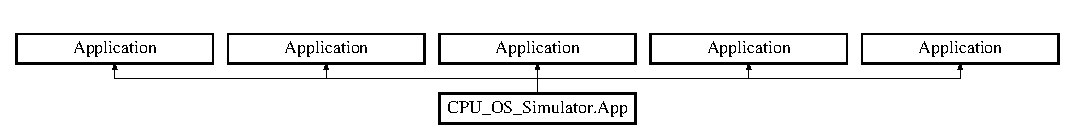
\includegraphics[height=2.000000cm]{class_c_p_u___o_s___simulator_1_1_app}
\end{center}
\end{figure}
\subsection*{Public Member Functions}
\begin{DoxyCompactItemize}
\item 
void \hyperlink{class_c_p_u___o_s___simulator_1_1_app_a15e2e0e02c8dbe7d5d3fba5d21f3e56f}{Initialize\+Component} ()
\begin{DoxyCompactList}\small\item\em Initialize\+Component \end{DoxyCompactList}\item 
void \hyperlink{class_c_p_u___o_s___simulator_1_1_app_a15e2e0e02c8dbe7d5d3fba5d21f3e56f}{Initialize\+Component} ()
\begin{DoxyCompactList}\small\item\em Initialize\+Component \end{DoxyCompactList}\end{DoxyCompactItemize}
\subsection*{Static Public Member Functions}
\begin{DoxyCompactItemize}
\item 
static void \hyperlink{class_c_p_u___o_s___simulator_1_1_app_a7bbb69f458b77923e336283b1653ce69}{Main} ()
\begin{DoxyCompactList}\small\item\em Application Entry Point. \end{DoxyCompactList}\item 
static void \hyperlink{class_c_p_u___o_s___simulator_1_1_app_a7bbb69f458b77923e336283b1653ce69}{Main} ()
\begin{DoxyCompactList}\small\item\em Application Entry Point. \end{DoxyCompactList}\end{DoxyCompactItemize}


\subsection{Detailed Description}
Interaction logic for App.\+xaml 

\hyperlink{class_c_p_u___o_s___simulator_1_1_app}{App} 

Definition at line 8 of file App.\+xaml.\+cs.



\subsection{Member Function Documentation}
\hypertarget{class_c_p_u___o_s___simulator_1_1_app_a15e2e0e02c8dbe7d5d3fba5d21f3e56f}{}\index{C\+P\+U\+\_\+\+O\+S\+\_\+\+Simulator\+::\+App@{C\+P\+U\+\_\+\+O\+S\+\_\+\+Simulator\+::\+App}!Initialize\+Component@{Initialize\+Component}}
\index{Initialize\+Component@{Initialize\+Component}!C\+P\+U\+\_\+\+O\+S\+\_\+\+Simulator\+::\+App@{C\+P\+U\+\_\+\+O\+S\+\_\+\+Simulator\+::\+App}}
\subsubsection[{Initialize\+Component()}]{\setlength{\rightskip}{0pt plus 5cm}void C\+P\+U\+\_\+\+O\+S\+\_\+\+Simulator.\+App.\+Initialize\+Component (
\begin{DoxyParamCaption}
{}
\end{DoxyParamCaption}
)}\label{class_c_p_u___o_s___simulator_1_1_app_a15e2e0e02c8dbe7d5d3fba5d21f3e56f}


Initialize\+Component 



Definition at line 48 of file App.\+g.\+cs.

\hypertarget{class_c_p_u___o_s___simulator_1_1_app_a15e2e0e02c8dbe7d5d3fba5d21f3e56f}{}\index{C\+P\+U\+\_\+\+O\+S\+\_\+\+Simulator\+::\+App@{C\+P\+U\+\_\+\+O\+S\+\_\+\+Simulator\+::\+App}!Initialize\+Component@{Initialize\+Component}}
\index{Initialize\+Component@{Initialize\+Component}!C\+P\+U\+\_\+\+O\+S\+\_\+\+Simulator\+::\+App@{C\+P\+U\+\_\+\+O\+S\+\_\+\+Simulator\+::\+App}}
\subsubsection[{Initialize\+Component()}]{\setlength{\rightskip}{0pt plus 5cm}void C\+P\+U\+\_\+\+O\+S\+\_\+\+Simulator.\+App.\+Initialize\+Component (
\begin{DoxyParamCaption}
{}
\end{DoxyParamCaption}
)}\label{class_c_p_u___o_s___simulator_1_1_app_a15e2e0e02c8dbe7d5d3fba5d21f3e56f}


Initialize\+Component 



Definition at line 48 of file App.\+g.\+i.\+cs.

\hypertarget{class_c_p_u___o_s___simulator_1_1_app_a7bbb69f458b77923e336283b1653ce69}{}\index{C\+P\+U\+\_\+\+O\+S\+\_\+\+Simulator\+::\+App@{C\+P\+U\+\_\+\+O\+S\+\_\+\+Simulator\+::\+App}!Main@{Main}}
\index{Main@{Main}!C\+P\+U\+\_\+\+O\+S\+\_\+\+Simulator\+::\+App@{C\+P\+U\+\_\+\+O\+S\+\_\+\+Simulator\+::\+App}}
\subsubsection[{Main()}]{\setlength{\rightskip}{0pt plus 5cm}static void C\+P\+U\+\_\+\+O\+S\+\_\+\+Simulator.\+App.\+Main (
\begin{DoxyParamCaption}
{}
\end{DoxyParamCaption}
)\hspace{0.3cm}{\ttfamily [static]}}\label{class_c_p_u___o_s___simulator_1_1_app_a7bbb69f458b77923e336283b1653ce69}


Application Entry Point. 



Definition at line 63 of file App.\+g.\+i.\+cs.

\hypertarget{class_c_p_u___o_s___simulator_1_1_app_a7bbb69f458b77923e336283b1653ce69}{}\index{C\+P\+U\+\_\+\+O\+S\+\_\+\+Simulator\+::\+App@{C\+P\+U\+\_\+\+O\+S\+\_\+\+Simulator\+::\+App}!Main@{Main}}
\index{Main@{Main}!C\+P\+U\+\_\+\+O\+S\+\_\+\+Simulator\+::\+App@{C\+P\+U\+\_\+\+O\+S\+\_\+\+Simulator\+::\+App}}
\subsubsection[{Main()}]{\setlength{\rightskip}{0pt plus 5cm}static void C\+P\+U\+\_\+\+O\+S\+\_\+\+Simulator.\+App.\+Main (
\begin{DoxyParamCaption}
{}
\end{DoxyParamCaption}
)\hspace{0.3cm}{\ttfamily [static]}}\label{class_c_p_u___o_s___simulator_1_1_app_a7bbb69f458b77923e336283b1653ce69}


Application Entry Point. 



Definition at line 63 of file App.\+g.\+cs.



The documentation for this class was generated from the following files\+:\begin{DoxyCompactItemize}
\item 
C\+P\+U-\/\+O\+S Simulator/\hyperlink{_app_8xaml_8cs}{App.\+xaml.\+cs}\item 
C\+P\+U-\/\+O\+S Simulator/obj/\+Debug/\hyperlink{_app_8g_8cs}{App.\+g.\+cs}\item 
C\+P\+U-\/\+O\+S Simulator/obj/\+Debug/\hyperlink{_app_8g_8i_8cs}{App.\+g.\+i.\+cs}\end{DoxyCompactItemize}

\hypertarget{class_c_p_u___o_s___simulator_1_1_main_window}{}\section{C\+P\+U\+\_\+\+O\+S\+\_\+\+Simulator.\+Main\+Window Class Reference}
\label{class_c_p_u___o_s___simulator_1_1_main_window}\index{C\+P\+U\+\_\+\+O\+S\+\_\+\+Simulator.\+Main\+Window@{C\+P\+U\+\_\+\+O\+S\+\_\+\+Simulator.\+Main\+Window}}


Interaction logic for Main\+Window.\+xaml  


Inheritance diagram for C\+P\+U\+\_\+\+O\+S\+\_\+\+Simulator.\+Main\+Window\+:\begin{figure}[H]
\begin{center}
\leavevmode
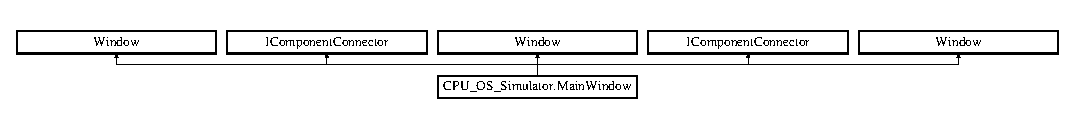
\includegraphics[height=11.000000cm]{class_c_p_u___o_s___simulator_1_1_main_window}
\end{center}
\end{figure}
\subsection*{Public Member Functions}
\begin{DoxyCompactItemize}
\item 
\hyperlink{class_c_p_u___o_s___simulator_1_1_main_window_a33462505a86657583c1560cbf02172bd}{Main\+Window} ()
\begin{DoxyCompactList}\small\item\em Constructor For the main window \end{DoxyCompactList}\item 
\hyperlink{class_c_p_u___o_s___simulator_1_1_c_p_u_1_1_instruction}{Instruction} \hyperlink{class_c_p_u___o_s___simulator_1_1_main_window_aeab49a3421f75049e47ed30b86bf8ad5}{Create\+Instruction} (\hyperlink{namespace_c_p_u___o_s___simulator_1_1_c_p_u_ac29c87bff87ad404c953b2581024043e}{Enum\+Opcodes} opcode, \hyperlink{class_c_p_u___o_s___simulator_1_1_c_p_u_1_1_operand}{Operand} op1, \hyperlink{class_c_p_u___o_s___simulator_1_1_c_p_u_1_1_operand}{Operand} op2, int Size)
\begin{DoxyCompactList}\small\item\em Creates an instruction with 2 operands \end{DoxyCompactList}\item 
\hyperlink{class_c_p_u___o_s___simulator_1_1_c_p_u_1_1_instruction}{Instruction} \hyperlink{class_c_p_u___o_s___simulator_1_1_main_window_a25a43c9a60f98f8196199d04420e48cf}{Create\+Instruction} (\hyperlink{namespace_c_p_u___o_s___simulator_1_1_c_p_u_ac29c87bff87ad404c953b2581024043e}{Enum\+Opcodes} opcode, \hyperlink{class_c_p_u___o_s___simulator_1_1_c_p_u_1_1_operand}{Operand} op1, int Size)
\begin{DoxyCompactList}\small\item\em Creates an instruction with 1 operand \end{DoxyCompactList}\item 
\hyperlink{class_c_p_u___o_s___simulator_1_1_c_p_u_1_1_instruction}{Instruction} \hyperlink{class_c_p_u___o_s___simulator_1_1_main_window_a608bc25c49d397aacde6cdd41d4314c3}{Create\+Instruction} (\hyperlink{namespace_c_p_u___o_s___simulator_1_1_c_p_u_ac29c87bff87ad404c953b2581024043e}{Enum\+Opcodes} opcode, int Size)
\begin{DoxyCompactList}\small\item\em Creates an instruction with no operands \end{DoxyCompactList}\item 
void \hyperlink{class_c_p_u___o_s___simulator_1_1_main_window_ae73f56ccee0f45b0df54438b3d397dd9}{Add\+Instruction} (\hyperlink{class_c_p_u___o_s___simulator_1_1_c_p_u_1_1_instruction}{Instruction} ins, int index)
\begin{DoxyCompactList}\small\item\em Adds an instruction to the currently loaded program \end{DoxyCompactList}\item 
void \hyperlink{class_c_p_u___o_s___simulator_1_1_main_window_a195e7715af146b207e5b973bd10c80c6}{Dispose} ()
\item 
void \hyperlink{class_c_p_u___o_s___simulator_1_1_main_window_a30724af44ae89c2172130c2dd36e145c}{Initialize\+Component} ()
\begin{DoxyCompactList}\small\item\em Initialize\+Component \end{DoxyCompactList}\item 
void \hyperlink{class_c_p_u___o_s___simulator_1_1_main_window_a30724af44ae89c2172130c2dd36e145c}{Initialize\+Component} ()
\begin{DoxyCompactList}\small\item\em Initialize\+Component \end{DoxyCompactList}\item 
void \hyperlink{class_c_p_u___o_s___simulator_1_1_main_window_a30724af44ae89c2172130c2dd36e145c}{Initialize\+Component} ()
\begin{DoxyCompactList}\small\item\em Initialize\+Component \end{DoxyCompactList}\item 
void \hyperlink{class_c_p_u___o_s___simulator_1_1_main_window_a30724af44ae89c2172130c2dd36e145c}{Initialize\+Component} ()
\begin{DoxyCompactList}\small\item\em Initialize\+Component \end{DoxyCompactList}\end{DoxyCompactItemize}
\subsection*{Public Attributes}
\begin{DoxyCompactItemize}
\item 
string \hyperlink{class_c_p_u___o_s___simulator_1_1_main_window_a91f063d9cf776004dc74e719ef942907}{current\+Program} = string.\+Empty
\end{DoxyCompactItemize}
\subsection*{Static Public Attributes}
\begin{DoxyCompactItemize}
\item 
static \hyperlink{class_c_p_u___o_s___simulator_1_1_main_window}{Main\+Window} \hyperlink{class_c_p_u___o_s___simulator_1_1_main_window_a1280266cc57403a91f08a8350dee05cc}{current\+Instance}
\end{DoxyCompactItemize}
\subsection*{Package Attributes}
\begin{DoxyCompactItemize}
\item 
\hyperlink{class_c_p_u___o_s___simulator_1_1_main_window}{C\+P\+U\+\_\+\+O\+S\+\_\+\+Simulator.\+Main\+Window} \hyperlink{class_c_p_u___o_s___simulator_1_1_main_window_adf996cda04d3cf426847b8fd8981ee66}{Main\+Window2}
\item 
System.\+Windows.\+Controls.\+Grid \hyperlink{class_c_p_u___o_s___simulator_1_1_main_window_a5c56d82a7b611446e81b7baa3229d76b}{Main\+Window\+Grid}
\item 
System.\+Windows.\+Controls.\+Grid \hyperlink{class_c_p_u___o_s___simulator_1_1_main_window_a2e6841673af413e8a8f8ba8aa0d7c80b}{Instructions\+Grid}
\item 
System.\+Windows.\+Controls.\+Group\+Box \hyperlink{class_c_p_u___o_s___simulator_1_1_main_window_aebc1256b654d001b7c4ce2bc08522667}{grp\+\_\+\+Instructions\+Box}
\item 
System.\+Windows.\+Controls.\+Grid \hyperlink{class_c_p_u___o_s___simulator_1_1_main_window_a94a99eeb7f5fcfcfbdc375937d5439e7}{Instructions\+Inner\+Grid}
\item 
System.\+Windows.\+Controls.\+List\+View \hyperlink{class_c_p_u___o_s___simulator_1_1_main_window_acdab094f589df9435fa8e3bfe04e61cb}{lst\+\_\+\+Instructions\+List}
\item 
System.\+Windows.\+Controls.\+Primitives.\+Scroll\+Bar \hyperlink{class_c_p_u___o_s___simulator_1_1_main_window_a014812a0e9cd159be05250d94d9a5a8b}{scroll\+Bar1}
\item 
System.\+Windows.\+Controls.\+Grid \hyperlink{class_c_p_u___o_s___simulator_1_1_main_window_ae4f2459995eb2f672c0fd3c2248b79fd}{Operations\+Grid}
\item 
System.\+Windows.\+Controls.\+Tab\+Control \hyperlink{class_c_p_u___o_s___simulator_1_1_main_window_a615ea960969aa9a61afdaef8cf039348}{Program\+Tab}
\item 
System.\+Windows.\+Controls.\+Group\+Box \hyperlink{class_c_p_u___o_s___simulator_1_1_main_window_a1e75e7af485b229372a6aafb84c2ffe0}{grp\+\_\+\+New\+Program}
\item 
System.\+Windows.\+Controls.\+Grid \hyperlink{class_c_p_u___o_s___simulator_1_1_main_window_a38bef5fa03edcca52fa7fc11068923bd}{grid\+\_\+\+New\+Program}
\item 
System.\+Windows.\+Controls.\+Label \hyperlink{class_c_p_u___o_s___simulator_1_1_main_window_ad60038602dcf5d954e420bee89c8494d}{label}
\item 
System.\+Windows.\+Controls.\+Text\+Box \hyperlink{class_c_p_u___o_s___simulator_1_1_main_window_a2c64b45db8c1d7a30c2f9155899cf918}{txt\+Program\+Name}
\item 
System.\+Windows.\+Controls.\+Label \hyperlink{class_c_p_u___o_s___simulator_1_1_main_window_a09b3ba374a620331bc447b32959260c2}{label1}
\item 
System.\+Windows.\+Controls.\+Text\+Box \hyperlink{class_c_p_u___o_s___simulator_1_1_main_window_aa6eeef1bfdd74aa90d6fea68987306ad}{txt\+Base\+Address}
\item 
System.\+Windows.\+Controls.\+Label \hyperlink{class_c_p_u___o_s___simulator_1_1_main_window_a88c7b6748a5e198c673a3c3c5178d3b8}{label2}
\item 
System.\+Windows.\+Controls.\+Combo\+Box \hyperlink{class_c_p_u___o_s___simulator_1_1_main_window_a8da421354f40baef03909c87c3407e3c}{cmb\+\_\+\+Pages}
\item 
System.\+Windows.\+Controls.\+Button \hyperlink{class_c_p_u___o_s___simulator_1_1_main_window_a4f0d9f8f3d56b76616367438d04b4fde}{btn\+\_\+\+Program\+Add}
\item 
System.\+Windows.\+Controls.\+Group\+Box \hyperlink{class_c_p_u___o_s___simulator_1_1_main_window_a2cafe5a8b54ae3e95a770abc594519a0}{grp\+\_\+\+Programs}
\item 
System.\+Windows.\+Controls.\+Grid \hyperlink{class_c_p_u___o_s___simulator_1_1_main_window_a7a4cb93db4cde3b227cbc3155af574d2}{grid\+\_\+\+Programs}
\item 
System.\+Windows.\+Controls.\+Button \hyperlink{class_c_p_u___o_s___simulator_1_1_main_window_a638eee3b21f6ac5d28a5c95c4dad3fc2}{btn\+\_\+\+Save}
\item 
System.\+Windows.\+Controls.\+Button \hyperlink{class_c_p_u___o_s___simulator_1_1_main_window_a29fbdb7afddedc9425472096337ee13b}{btn\+\_\+\+Load}
\item 
System.\+Windows.\+Controls.\+Button \hyperlink{class_c_p_u___o_s___simulator_1_1_main_window_ad56a38e017d6d47d2076b1ec33e3521d}{btn\+\_\+\+Copy\+To\+Clipboard}
\item 
System.\+Windows.\+Controls.\+Label \hyperlink{class_c_p_u___o_s___simulator_1_1_main_window_a9cbfc378965cf635e61c760e11dd5c8a}{lbl\+Program\+List}
\item 
System.\+Windows.\+Controls.\+Combo\+Box \hyperlink{class_c_p_u___o_s___simulator_1_1_main_window_a9871f5933923725d4386a7a7f3f8828f}{cmb\+\_\+\+Program\+List}
\item 
System.\+Windows.\+Controls.\+Label \hyperlink{class_c_p_u___o_s___simulator_1_1_main_window_ae3adff2ef98d792ce094dcc229c293a8}{lbl\+\_\+\+Base\+Address}
\item 
System.\+Windows.\+Controls.\+Text\+Box \hyperlink{class_c_p_u___o_s___simulator_1_1_main_window_ae6c0ce6078d081b2cb99518c68f1cd85}{txt\+Load\+Base\+Address}
\item 
System.\+Windows.\+Controls.\+Check\+Box \hyperlink{class_c_p_u___o_s___simulator_1_1_main_window_a8ade8cf3e5e2ec2374c984dac406b5e9}{chk\+\_\+\+Load\+Base\+Address}
\item 
System.\+Windows.\+Controls.\+Tab\+Item \hyperlink{class_c_p_u___o_s___simulator_1_1_main_window_a4fe9f6d97eb1f2c45b9e5a0363e61557}{Instruction\+Tab}
\item 
System.\+Windows.\+Controls.\+Grid \hyperlink{class_c_p_u___o_s___simulator_1_1_main_window_af09ff1f305e936227c4a975f4c788133}{grid\+\_\+\+Instructions}
\item 
System.\+Windows.\+Controls.\+Button \hyperlink{class_c_p_u___o_s___simulator_1_1_main_window_a50fb8fcd9e592c4987fac4bcb8762785}{btn\+\_\+\+Add\+New}
\item 
System.\+Windows.\+Controls.\+Button \hyperlink{class_c_p_u___o_s___simulator_1_1_main_window_a3c6c4760a8fd64f653fff0ad06374f13}{btn\+\_\+\+Show}
\item 
System.\+Windows.\+Controls.\+Button \hyperlink{class_c_p_u___o_s___simulator_1_1_main_window_ac30720a1b345a3d59312d2d68f742359}{btn\+\_\+\+Undo}
\item 
System.\+Windows.\+Controls.\+Button \hyperlink{class_c_p_u___o_s___simulator_1_1_main_window_a23c681375b103d2294ac79c51f1fb406}{btn\+\_\+\+Insert\+Above}
\item 
System.\+Windows.\+Controls.\+Button \hyperlink{class_c_p_u___o_s___simulator_1_1_main_window_ac6bfabebf21c92a905764305b789df46}{btn\+Move\+Down}
\item 
System.\+Windows.\+Controls.\+Button \hyperlink{class_c_p_u___o_s___simulator_1_1_main_window_ae07013ea273fb1e9f38fd1dd83144371}{btn\+\_\+\+Edit}
\item 
System.\+Windows.\+Controls.\+Button \hyperlink{class_c_p_u___o_s___simulator_1_1_main_window_a7c6c417d0bd3af11e77f86cf2cfb03fe}{btn\+\_\+\+Insert\+Below}
\item 
System.\+Windows.\+Controls.\+Button \hyperlink{class_c_p_u___o_s___simulator_1_1_main_window_aa85d9301fed773f44a352aad64a9d80d}{btn\+Move\+Up}
\item 
System.\+Windows.\+Controls.\+Button \hyperlink{class_c_p_u___o_s___simulator_1_1_main_window_a74623b1e8f8ab1b3b6835bda2e8a9256}{btn\+\_\+\+Delete}
\item 
System.\+Windows.\+Controls.\+Button \hyperlink{class_c_p_u___o_s___simulator_1_1_main_window_a55b2516a7b78d0e79deac7f1a79f3a92}{btn\+\_\+\+Copy}
\item 
System.\+Windows.\+Controls.\+Button \hyperlink{class_c_p_u___o_s___simulator_1_1_main_window_ae2ef9b73d0b5776415c7f3e91c1eaf21}{btn\+Paste\+Above}
\item 
System.\+Windows.\+Controls.\+Button \hyperlink{class_c_p_u___o_s___simulator_1_1_main_window_a1c24521ff648d75bf5991567e1a85b55}{btn\+\_\+\+Paste\+Below}
\item 
System.\+Windows.\+Controls.\+Tab\+Item \hyperlink{class_c_p_u___o_s___simulator_1_1_main_window_a47b1359d9e96abf2b0935eb3392405d4}{Optimize\+Tab}
\item 
System.\+Windows.\+Controls.\+Grid \hyperlink{class_c_p_u___o_s___simulator_1_1_main_window_adb8397cdbc794d18b0379ba7251d2278}{Program\+List\+Grid}
\item 
System.\+Windows.\+Controls.\+Group\+Box \hyperlink{class_c_p_u___o_s___simulator_1_1_main_window_a0ccd227c10c9a0878095ef10c0ff92b7}{grp\+\_\+\+Program\+List}
\item 
System.\+Windows.\+Controls.\+Grid \hyperlink{class_c_p_u___o_s___simulator_1_1_main_window_a4e287cef9f0becaebe0777af8de2d8c9}{Program\+List\+View\+Grid}
\item 
System.\+Windows.\+Controls.\+List\+View \hyperlink{class_c_p_u___o_s___simulator_1_1_main_window_ab33f21e0f19eab104e6f67f44d89daeb}{lst\+\_\+\+Program\+List}
\item 
System.\+Windows.\+Controls.\+Button \hyperlink{class_c_p_u___o_s___simulator_1_1_main_window_af2d1c3293ffaa1d203a9bdb8bf282eab}{btn\+\_\+\+Show\+Memory}
\item 
System.\+Windows.\+Controls.\+Grid \hyperlink{class_c_p_u___o_s___simulator_1_1_main_window_a37acb139db0aa54950350fdb47dfd452}{Register\+Grid}
\item 
System.\+Windows.\+Controls.\+Group\+Box \hyperlink{class_c_p_u___o_s___simulator_1_1_main_window_af858add509dfe2b90f0d356822f73737}{grp\+\_\+\+Registers}
\item 
System.\+Windows.\+Controls.\+Grid \hyperlink{class_c_p_u___o_s___simulator_1_1_main_window_a27d2d9e2ed92e2daa444ca8086a0861e}{Register\+Inner\+Grid}
\item 
System.\+Windows.\+Controls.\+List\+View \hyperlink{class_c_p_u___o_s___simulator_1_1_main_window_ae88013c536662328670f206a4cab99b1}{lst\+\_\+\+Registers}
\item 
System.\+Windows.\+Controls.\+Grid \hyperlink{class_c_p_u___o_s___simulator_1_1_main_window_a7ce98e44f9236ca31eb5bf3ed81c3372}{Special\+Registers\+Grid}
\item 
System.\+Windows.\+Controls.\+Group\+Box \hyperlink{class_c_p_u___o_s___simulator_1_1_main_window_a02e4a81d8689928cb1d459fd3c01bfdf}{grp\+\_\+\+Special\+Registers}
\item 
System.\+Windows.\+Controls.\+Grid \hyperlink{class_c_p_u___o_s___simulator_1_1_main_window_aeef1e97d3e7d589fdab51828260c7b5a}{Special\+Registers\+Inner\+Grid}
\item 
System.\+Windows.\+Controls.\+Label \hyperlink{class_c_p_u___o_s___simulator_1_1_main_window_a94cf4fbdaebb09776745893c2bce1126}{label3}
\item 
System.\+Windows.\+Controls.\+Text\+Box \hyperlink{class_c_p_u___o_s___simulator_1_1_main_window_a7100765f8e26fa4c97a76dd445942b97}{txt\+\_\+\+P\+C}
\item 
System.\+Windows.\+Controls.\+Label \hyperlink{class_c_p_u___o_s___simulator_1_1_main_window_a3473dc873d8c8d8f4bba6e83f5684299}{label4}
\item 
System.\+Windows.\+Controls.\+Text\+Box \hyperlink{class_c_p_u___o_s___simulator_1_1_main_window_a9135c01bacd48e517d7cf46f69ea87d2}{txt\+\_\+\+S\+R}
\item 
System.\+Windows.\+Controls.\+Label \hyperlink{class_c_p_u___o_s___simulator_1_1_main_window_a37b18e7542e985a8984375d0b1cf441e}{label5}
\item 
System.\+Windows.\+Controls.\+Text\+Box \hyperlink{class_c_p_u___o_s___simulator_1_1_main_window_ac2427655774b9ca2b4c368651d5cd9de}{txt\+\_\+\+S\+P}
\item 
System.\+Windows.\+Controls.\+Label \hyperlink{class_c_p_u___o_s___simulator_1_1_main_window_aadfe7782d7e25b730849222805a541f9}{label5\+\_\+\+Copy}
\item 
System.\+Windows.\+Controls.\+Text\+Box \hyperlink{class_c_p_u___o_s___simulator_1_1_main_window_a7a878022ed4cb948598d3685dc821a00}{txt\+\_\+\+B\+R}
\item 
System.\+Windows.\+Controls.\+Group\+Box \hyperlink{class_c_p_u___o_s___simulator_1_1_main_window_a9947d1946c8258ea1fb77d860baa7e0f}{grp\+\_\+\+Status\+Flags}
\item 
System.\+Windows.\+Controls.\+Grid \hyperlink{class_c_p_u___o_s___simulator_1_1_main_window_afdda5e5a39c6e3b99300284ea2640e7c}{Status\+Flags\+Grid}
\item 
System.\+Windows.\+Controls.\+Check\+Box \hyperlink{class_c_p_u___o_s___simulator_1_1_main_window_adfbc519740506214093673b8015ea67d}{chk\+\_\+\+O\+V}
\item 
System.\+Windows.\+Controls.\+Check\+Box \hyperlink{class_c_p_u___o_s___simulator_1_1_main_window_a70c1a75df218201391cf5e0615a600f1}{chk\+\_\+\+Z}
\item 
System.\+Windows.\+Controls.\+Check\+Box \hyperlink{class_c_p_u___o_s___simulator_1_1_main_window_ab8a23e33c5c71e359574de36ccf8d991}{chk\+\_\+\+N}
\item 
System.\+Windows.\+Controls.\+Group\+Box \hyperlink{class_c_p_u___o_s___simulator_1_1_main_window_a0e549bad0f6778b2ea3fffb6c2d1a2bb}{grp\+\_\+\+C\+P\+U\+Mode}
\item 
System.\+Windows.\+Controls.\+Grid \hyperlink{class_c_p_u___o_s___simulator_1_1_main_window_ab6afb45d3f05517e9df6af167752be77}{C\+P\+U\+Mode\+Grid}
\item 
System.\+Windows.\+Controls.\+Radio\+Button \hyperlink{class_c_p_u___o_s___simulator_1_1_main_window_ab9e8d52c337bc24a24d8282dfbf449c8}{rdb\+\_\+\+User}
\item 
System.\+Windows.\+Controls.\+Radio\+Button \hyperlink{class_c_p_u___o_s___simulator_1_1_main_window_a549c6be690b051f4ab15dce643dec656}{rdb\+\_\+\+Kernel}
\item 
System.\+Windows.\+Controls.\+Label \hyperlink{class_c_p_u___o_s___simulator_1_1_main_window_a8f210008776bb163b4c2c2b160aa52be}{label6}
\item 
System.\+Windows.\+Controls.\+Text\+Box \hyperlink{class_c_p_u___o_s___simulator_1_1_main_window_ac6e0cfcdd72688d7bffd100ce6d11a28}{txt\+\_\+\+I\+R}
\item 
System.\+Windows.\+Controls.\+Label \hyperlink{class_c_p_u___o_s___simulator_1_1_main_window_a18612502a8ab2d53d85434e426785022}{label6\+\_\+\+Copy}
\item 
System.\+Windows.\+Controls.\+Text\+Box \hyperlink{class_c_p_u___o_s___simulator_1_1_main_window_a87f8440246e9f6ace0aa4d69b5bba289}{txt\+\_\+\+M\+A\+R}
\item 
System.\+Windows.\+Controls.\+Label \hyperlink{class_c_p_u___o_s___simulator_1_1_main_window_a890bd54d36af19ec881b6a840d6ac8a9}{label6\+\_\+\+Copy1}
\item 
System.\+Windows.\+Controls.\+Text\+Box \hyperlink{class_c_p_u___o_s___simulator_1_1_main_window_a1aa53d1512aa84e476b3649dcda5ced0}{txt\+\_\+\+M\+D\+R}
\item 
System.\+Windows.\+Controls.\+Grid \hyperlink{class_c_p_u___o_s___simulator_1_1_main_window_a59373e8f8822e4efea670d9fb87a1b32}{Program\+Stack\+Grid}
\item 
System.\+Windows.\+Controls.\+Group\+Box \hyperlink{class_c_p_u___o_s___simulator_1_1_main_window_a10687b397ff3a0381a556096a14ed0b0}{grp\+\_\+\+Program\+Stack}
\item 
System.\+Windows.\+Controls.\+Grid \hyperlink{class_c_p_u___o_s___simulator_1_1_main_window_a8c373866c86f6be0e7ef487a5ccb8c3c}{Program\+Stack\+Inner\+Grid}
\item 
System.\+Windows.\+Controls.\+List\+View \hyperlink{class_c_p_u___o_s___simulator_1_1_main_window_a8453db331c7cc1e7c1e711a06b2ec30c}{lst\+\_\+\+Stack}
\item 
System.\+Windows.\+Controls.\+Grid \hyperlink{class_c_p_u___o_s___simulator_1_1_main_window_af6e1d9a71f9501c02b62e8319ba11b5a}{Control\+Unit\+Grid}
\item 
System.\+Windows.\+Controls.\+Tab\+Control \hyperlink{class_c_p_u___o_s___simulator_1_1_main_window_acc893fc507d9ea08cc4a923bdc23091d}{Control\+Tabs}
\item 
System.\+Windows.\+Controls.\+Grid \hyperlink{class_c_p_u___o_s___simulator_1_1_main_window_a0bb4b4233380c349ee3bef69813a684b}{Control\+Unit\+Inner\+Grid}
\item 
System.\+Windows.\+Controls.\+Button \hyperlink{class_c_p_u___o_s___simulator_1_1_main_window_acd572aa9d278af703febb634fc1c34a3}{btn\+\_\+\+Step}
\item 
System.\+Windows.\+Controls.\+Button \hyperlink{class_c_p_u___o_s___simulator_1_1_main_window_ab3286e931d7154605876654bbf092840}{btn\+\_\+\+Run}
\item 
System.\+Windows.\+Controls.\+Button \hyperlink{class_c_p_u___o_s___simulator_1_1_main_window_a1b6b541d9765ca230f537d1d6b6c83aa}{btn\+\_\+\+Stop}
\item 
System.\+Windows.\+Controls.\+Radio\+Button \hyperlink{class_c_p_u___o_s___simulator_1_1_main_window_acba6218f7f716645443533815c6bd7a3}{rdb\+\_\+\+By\+Instruction}
\item 
System.\+Windows.\+Controls.\+Radio\+Button \hyperlink{class_c_p_u___o_s___simulator_1_1_main_window_ab40dcb618f5398ab67213476fe1b86ca}{rdb\+\_\+\+By\+Single\+Tick}
\item 
System.\+Windows.\+Controls.\+Slider \hyperlink{class_c_p_u___o_s___simulator_1_1_main_window_a39cd3af9bb0f8a3ccd06fdd44c9ed6a3}{sld\+\_\+\+Clock\+Speed}
\item 
System.\+Windows.\+Controls.\+Label \hyperlink{class_c_p_u___o_s___simulator_1_1_main_window_a38ed6363fd03954967bda7a099f6b07e}{label7}
\item 
System.\+Windows.\+Controls.\+Label \hyperlink{class_c_p_u___o_s___simulator_1_1_main_window_a216fc6a1692d8a8f8b80b08348c1dcd4}{label8}
\item 
System.\+Windows.\+Controls.\+Button \hyperlink{class_c_p_u___o_s___simulator_1_1_main_window_ada16565fc869dea1d54013009f5892b4}{btn\+\_\+\+Reset\+Program}
\item 
System.\+Windows.\+Controls.\+Button \hyperlink{class_c_p_u___o_s___simulator_1_1_main_window_a967a1b3dbde7ecb1d8091e5eababcc58}{btn\+\_\+\+Show\+P\+C\+B}
\item 
System.\+Windows.\+Controls.\+Grid \hyperlink{class_c_p_u___o_s___simulator_1_1_main_window_a65cbc082cd4737ec0dd8837efa715510}{grid\+\_\+\+Advanced}
\item 
System.\+Windows.\+Controls.\+Tab\+Control \hyperlink{class_c_p_u___o_s___simulator_1_1_main_window_a409f822cf5503ff0a45e14fb0f86a2aa}{advanced\+\_\+\+Tabs}
\item 
System.\+Windows.\+Controls.\+Tab\+Item \hyperlink{class_c_p_u___o_s___simulator_1_1_main_window_aa0cf25219ff7ec68cccc82f780e5f817}{advanced\+\_\+\+Tab}
\item 
System.\+Windows.\+Controls.\+Grid \hyperlink{class_c_p_u___o_s___simulator_1_1_main_window_a50b3891532cc5bfd0cc44e657bf95374}{advanced\+\_\+\+Grid}
\item 
System.\+Windows.\+Controls.\+Button \hyperlink{class_c_p_u___o_s___simulator_1_1_main_window_a9c127982ee67a80b67a9184b3a6e83d3}{btn\+\_\+\+Console}
\end{DoxyCompactItemize}
\subsection*{Properties}
\begin{DoxyCompactItemize}
\item 
List$<$ \hyperlink{class_c_p_u___o_s___simulator_1_1_c_p_u_1_1_simulator_program}{Simulator\+Program} $>$ \hyperlink{class_c_p_u___o_s___simulator_1_1_main_window_a632c91cdd16a7498bbb8dfb3e5df252c}{Program\+List}\hspace{0.3cm}{\ttfamily  \mbox{[}get, set\mbox{]}}
\item 
\hyperlink{namespace_c_p_u___o_s___simulator_adc17a5a5e004084f05dc8e4d3f70e31f}{Enum\+Instruction\+Mode} \hyperlink{class_c_p_u___o_s___simulator_1_1_main_window_a65916937137002c26f9eb1c88cfff519}{Instruction\+Mode}\hspace{0.3cm}{\ttfamily  \mbox{[}get, set\mbox{]}}
\item 
\hyperlink{class_c_p_u___o_s___simulator_1_1_c_p_u_1_1_execution_unit}{Execution\+Unit} \hyperlink{class_c_p_u___o_s___simulator_1_1_main_window_a3d03550a73d7ab18ebd143a38dbf1431}{Active\+Unit}\hspace{0.3cm}{\ttfamily  \mbox{[}get, set\mbox{]}}
\item 
\hyperlink{class_c_p_u___o_s___simulator_1_1_memory_1_1_physical_memory}{Physical\+Memory} \hyperlink{class_c_p_u___o_s___simulator_1_1_main_window_abee63f1a7c5feecf97e7253a65806a5a}{Memory}\hspace{0.3cm}{\ttfamily  \mbox{[}get, set\mbox{]}}
\item 
\hyperlink{class_c_p_u___o_s___simulator_1_1_memory_1_1_swap_space}{Swap\+Space} \hyperlink{class_c_p_u___o_s___simulator_1_1_main_window_a114d0bf1ca63b0d9213537758535aecf}{Swap\+Space}\hspace{0.3cm}{\ttfamily  \mbox{[}get, set\mbox{]}}
\item 
Background\+Worker \hyperlink{class_c_p_u___o_s___simulator_1_1_main_window_aab5d6c95426ebe1e75b7c3bfc0488b84}{Execution\+Worker}\hspace{0.3cm}{\ttfamily  \mbox{[}get, set\mbox{]}}
\end{DoxyCompactItemize}
\subsection*{Private Member Functions}
\begin{DoxyCompactItemize}
\item 
static void \hyperlink{class_c_p_u___o_s___simulator_1_1_main_window_a0bbdb2d3b0e818f2d264770168521059}{S\+H\+Change\+Notify} (uint w\+Event\+Id, uint u\+Flags, Int\+Ptr dw\+Item1, Int\+Ptr dw\+Item2)
\item 
void \hyperlink{class_c_p_u___o_s___simulator_1_1_main_window_a06b2ba04e8c006037cae7b0e40b9c5a0}{Populate\+Registers} ()
\begin{DoxyCompactList}\small\item\em This function populates the register display in the main window \end{DoxyCompactList}\item 
void \hyperlink{class_c_p_u___o_s___simulator_1_1_main_window_a4fbca2d50698a847da4ab82c3f380680}{Update\+Registers} ()
\begin{DoxyCompactList}\small\item\em This function updates the register display in the main window whenever a register value is updated \end{DoxyCompactList}\item 
void \hyperlink{class_c_p_u___o_s___simulator_1_1_main_window_a798838ad3fae6117c8e624047a591931}{Update\+Special\+Registers} ()
\begin{DoxyCompactList}\small\item\em This function updates the values in the U\+I for the special registers \end{DoxyCompactList}\item 
void \hyperlink{class_c_p_u___o_s___simulator_1_1_main_window_a3b945b691332686989cd5b5107f7f98b}{Main\+Window2\+\_\+\+Loaded} (object sender, Routed\+Event\+Args e)
\item 
void \hyperlink{class_c_p_u___o_s___simulator_1_1_main_window_abe3e79941789134ce080390fcafc720e}{btn\+\_\+\+Program\+Add\+\_\+\+Click} (object sender, Routed\+Event\+Args e)
\begin{DoxyCompactList}\small\item\em Creates and adds a program to the program list \end{DoxyCompactList}\item 
\hyperlink{class_c_p_u___o_s___simulator_1_1_c_p_u_1_1_simulator_program}{Simulator\+Program} \hyperlink{class_c_p_u___o_s___simulator_1_1_main_window_a4cb75cfa224757b1dc708b60681ad803}{Create\+New\+Program} ()
\begin{DoxyCompactList}\small\item\em Creates a new program based on entered data \end{DoxyCompactList}\item 
\hyperlink{class_c_p_u___o_s___simulator_1_1_c_p_u_1_1_simulator_program}{Simulator\+Program} \hyperlink{class_c_p_u___o_s___simulator_1_1_main_window_aa735efa9bc97df2ceb545fdce5f351df}{Create\+New\+Program} (string program\+Name, int base\+Address, int pages)
\begin{DoxyCompactList}\small\item\em Creates a new program based on entered data \end{DoxyCompactList}\item 
void \hyperlink{class_c_p_u___o_s___simulator_1_1_main_window_afcb6e2b3719374f56fd8cb1c786bb219}{btn\+\_\+\+Show\+\_\+\+Click} (object sender, Routed\+Event\+Args e)
\begin{DoxyCompactList}\small\item\em Called when the show button is clicked \end{DoxyCompactList}\item 
void \hyperlink{class_c_p_u___o_s___simulator_1_1_main_window_a37c97ac2869b40063089f1af9cd86724}{btn\+\_\+\+Add\+New\+\_\+\+Click} (object sender, Routed\+Event\+Args e)
\begin{DoxyCompactList}\small\item\em Adds a new instruction to the program \end{DoxyCompactList}\item 
void \hyperlink{class_c_p_u___o_s___simulator_1_1_main_window_a8f710b1bee7b3c9360fb5652231b0502}{btn\+\_\+\+Insert\+Above\+\_\+\+Click} (object sender, Routed\+Event\+Args e)
\begin{DoxyCompactList}\small\item\em Adds a new instruction to the program above the selected instruction \end{DoxyCompactList}\item 
void \hyperlink{class_c_p_u___o_s___simulator_1_1_main_window_ac2307db4caedc82b5a6201077fb1c5b7}{btn\+\_\+\+Insert\+Below\+\_\+\+Click} (object sender, Routed\+Event\+Args e)
\begin{DoxyCompactList}\small\item\em Adds a new instruction to the program above below selected instruction \end{DoxyCompactList}\item 
void \hyperlink{class_c_p_u___o_s___simulator_1_1_main_window_a96ea1acde80b84701b58c1d4aaed2b9f}{btn\+\_\+\+Delete\+\_\+\+Click} (object sender, Routed\+Event\+Args e)
\begin{DoxyCompactList}\small\item\em Deletes the selected instruction from the program \end{DoxyCompactList}\item 
void \hyperlink{class_c_p_u___o_s___simulator_1_1_main_window_a622fd6a40ff66a4a87c3d31ccef4313c}{Main\+Window2\+\_\+\+Closing} (object sender, Cancel\+Event\+Args e)
\begin{DoxyCompactList}\small\item\em Called when the window is closing \end{DoxyCompactList}\item 
void \hyperlink{class_c_p_u___o_s___simulator_1_1_main_window_a5013d1984fc170246a5dc0d26c6fc493}{lst\+\_\+\+Instructions\+List\+\_\+\+Selection\+Changed} (object sender, Selection\+Changed\+Event\+Args e)
\item 
void \hyperlink{class_c_p_u___o_s___simulator_1_1_main_window_ab563b461cf3d62bd3c88eeb7921bfa75}{lst\+\_\+\+Program\+List\+\_\+\+Selection\+Changed} (object sender, Selection\+Changed\+Event\+Args e)
\item 
void \hyperlink{class_c_p_u___o_s___simulator_1_1_main_window_abd01bb7788b0c104045bcc93cf03c9d6}{Update\+Stack} ()
\begin{DoxyCompactList}\small\item\em This function updates the stack display in the main window whenever a value is pushed or popped from the stack \end{DoxyCompactList}\item 
void \hyperlink{class_c_p_u___o_s___simulator_1_1_main_window_a677bf9ebdb9fe30caa0f52f93e5390c9}{Update\+Intructions} ()
\begin{DoxyCompactList}\small\item\em Updates the list of instructions \end{DoxyCompactList}\item 
void \hyperlink{class_c_p_u___o_s___simulator_1_1_main_window_a13c54c19f906fc84076fe654f82f5398}{btn\+\_\+\+Load\+\_\+\+Click} (object sender, Routed\+Event\+Args e)
\item 
void \hyperlink{class_c_p_u___o_s___simulator_1_1_main_window_a3bbf0774868d6b5da4ff08d70e236fa6}{btn\+\_\+\+Save\+\_\+\+Click} (object sender, Routed\+Event\+Args e)
\item 
bool \hyperlink{class_c_p_u___o_s___simulator_1_1_main_window_a843bbe93c5c2225820d216cc1cb7d4e9}{Save\+Program} ()
\begin{DoxyCompactList}\small\item\em Saves the program list to a file \end{DoxyCompactList}\item 
bool \hyperlink{class_c_p_u___o_s___simulator_1_1_main_window_ad788d74c9d6582f3302912cbbba410b0}{Load\+Program} ()
\begin{DoxyCompactList}\small\item\em Loads a program list from a file \end{DoxyCompactList}\item 
void \hyperlink{class_c_p_u___o_s___simulator_1_1_main_window_a80985670e45349866a463b766f92e27b}{Serialize\+Object$<$ T $>$} (T serializable\+Object, string file\+Path)
\begin{DoxyCompactList}\small\item\em Serializes a program List. \end{DoxyCompactList}\item 
void \hyperlink{class_c_p_u___o_s___simulator_1_1_main_window_a44e09f35524cd53ddab77488989c5833}{De\+Serialize\+Object$<$ T $>$} (string file\+Name)
\begin{DoxyCompactList}\small\item\em De-\/serializes an .sas file into a program list \end{DoxyCompactList}\item 
void \hyperlink{class_c_p_u___o_s___simulator_1_1_main_window_afe4c815db0eb51ebc480374f5af09d0c}{Bind\+Instruction\+Delegates} (ref \hyperlink{class_c_p_u___o_s___simulator_1_1_c_p_u_1_1_simulator_program}{Simulator\+Program} prog)
\begin{DoxyCompactList}\small\item\em This function rebinds the delegate function to each instruction in a program after it is loaded from a file. \end{DoxyCompactList}\item 
void \hyperlink{class_c_p_u___o_s___simulator_1_1_main_window_ace253c0b4beef8898af97df25666df2f}{sld\+\_\+\+Clock\+Speed\+\_\+\+Value\+Changed} (object sender, Routed\+Property\+Changed\+Event\+Args$<$ double $>$ e)
\item 
void \hyperlink{class_c_p_u___o_s___simulator_1_1_main_window_a897049d123dd2ecf2820b02205ce1969}{btn\+\_\+\+Step\+\_\+\+Click} (object sender, Routed\+Event\+Args e)
\item 
void \hyperlink{class_c_p_u___o_s___simulator_1_1_main_window_a1f4dedca9ad81ea1c92637759515797f}{btn\+\_\+\+Run\+\_\+\+Click} (object sender, Routed\+Event\+Args e)
\item 
void \hyperlink{class_c_p_u___o_s___simulator_1_1_main_window_ad225bd7394d6ad45de9db58b562b91f7}{Create\+Background\+Worker} ()
\begin{DoxyCompactList}\small\item\em Creates a background worker for the execution thread to run on \end{DoxyCompactList}\item 
async void \hyperlink{class_c_p_u___o_s___simulator_1_1_main_window_a27c9bde14aab0b0a82f5e13e0a71c86c}{Update\+Interface} (object sender, Progress\+Changed\+Event\+Args e)
\begin{DoxyCompactList}\small\item\em Asynchronous method called after every instruction is executed to update required values and user interface asynchronously \end{DoxyCompactList}\item 
void \hyperlink{class_c_p_u___o_s___simulator_1_1_main_window_a83ba6352a96515569978030013c84b72}{Create\+Execution\+Thread} (object sender, Do\+Work\+Event\+Args e)
\item 
async Task$<$ int $>$ \hyperlink{class_c_p_u___o_s___simulator_1_1_main_window_adbb759abbf37061f785e82a9e7f7b3e1}{Update\+Interface} ()
\begin{DoxyCompactList}\small\item\em Asynchronous method called after every instruction is executed to update required values and user interface asynchronously \end{DoxyCompactList}\item 
async void \hyperlink{class_c_p_u___o_s___simulator_1_1_main_window_a03d4ec6b5990ad572db709f5305dd7ca}{Execute\+Program} (object program)
\begin{DoxyCompactList}\small\item\em Asynchronous method called to begin executing a program on the execution thread \end{DoxyCompactList}\item 
async Task$<$ int $>$ \hyperlink{class_c_p_u___o_s___simulator_1_1_main_window_a0712c91c3a03a4fabc2cdb2f4ed0a33b}{Call\+From\+Main\+Thread} (Func$<$ Task$<$ int $>$$>$ Function\+Pointer)
\begin{DoxyCompactList}\small\item\em Bridge function used to call functions on the main thread from within the background thread \end{DoxyCompactList}\item 
async Task$<$ string $>$ \hyperlink{class_c_p_u___o_s___simulator_1_1_main_window_ac30c6f157890cb452dc35ec851cc88ad}{Calculate\+Time} (long mills)
\begin{DoxyCompactList}\small\item\em This function calculates the time in seconds the last program took to execute \end{DoxyCompactList}\item 
void \hyperlink{class_c_p_u___o_s___simulator_1_1_main_window_acbdc92abd94c317f978cee0d28af9448}{btn\+\_\+\+Stop\+\_\+\+Click} (object sender, Routed\+Event\+Args e)
\item 
void \hyperlink{class_c_p_u___o_s___simulator_1_1_main_window_a524b638c053cd53f17e44fe225b9dd4f}{btn\+\_\+\+Reset\+Program\+\_\+\+Click} (object sender, Routed\+Event\+Args e)
\item 
void \hyperlink{class_c_p_u___o_s___simulator_1_1_main_window_a19b793a858804e5f7a5611603aeeaf79}{chk\+\_\+\+O\+V\+\_\+\+Checked} (object sender, Routed\+Event\+Args e)
\item 
void \hyperlink{class_c_p_u___o_s___simulator_1_1_main_window_a59f718f48699e2f35c0151057407c38c}{chk\+\_\+\+O\+V\+\_\+\+Unchecked} (object sender, Routed\+Event\+Args e)
\item 
void \hyperlink{class_c_p_u___o_s___simulator_1_1_main_window_ae6186ab1f27e668a1332b7cf72c70f19}{chk\+\_\+\+Z\+\_\+\+Checked} (object sender, Routed\+Event\+Args e)
\item 
void \hyperlink{class_c_p_u___o_s___simulator_1_1_main_window_a21d19250773a14a89aa8285dbe914c22}{chk\+\_\+\+Z\+\_\+\+Unchecked} (object sender, Routed\+Event\+Args e)
\item 
void \hyperlink{class_c_p_u___o_s___simulator_1_1_main_window_a0d0fff66a2f20f19e86f7d8d25aa8915}{chk\+\_\+\+N\+\_\+\+Checked} (object sender, Routed\+Event\+Args e)
\item 
void \hyperlink{class_c_p_u___o_s___simulator_1_1_main_window_afd6ed1a3f1774365c49977ca74daa906}{chk\+\_\+\+N\+\_\+\+Unchecked} (object sender, Routed\+Event\+Args e)
\item 
void \hyperlink{class_c_p_u___o_s___simulator_1_1_main_window_ae0466b84cb9b9aae5c60fe798585b5ed}{btn\+\_\+\+Show\+Memory\+\_\+\+Click} (object sender, Routed\+Event\+Args e)
\item 
void \hyperlink{class_c_p_u___o_s___simulator_1_1_main_window_a48b0283e10f83b8ab7b694ebd0410dd2}{btn\+\_\+\+Console\+\_\+\+Click} (object sender, Routed\+Event\+Args e)
\item 
void System.\+Windows.\+Markup.\+I\+Component\+Connector. \hyperlink{class_c_p_u___o_s___simulator_1_1_main_window_ae66177a5319cf24975b9dfab71bc830e}{Connect} (int connection\+Id, object target)
\item 
void System.\+Windows.\+Markup.\+I\+Component\+Connector. \hyperlink{class_c_p_u___o_s___simulator_1_1_main_window_ae66177a5319cf24975b9dfab71bc830e}{Connect} (int connection\+Id, object target)
\item 
void System.\+Windows.\+Markup.\+I\+Component\+Connector. \hyperlink{class_c_p_u___o_s___simulator_1_1_main_window_ae66177a5319cf24975b9dfab71bc830e}{Connect} (int connection\+Id, object target)
\item 
void System.\+Windows.\+Markup.\+I\+Component\+Connector. \hyperlink{class_c_p_u___o_s___simulator_1_1_main_window_ae66177a5319cf24975b9dfab71bc830e}{Connect} (int connection\+Id, object target)
\end{DoxyCompactItemize}
\subsection*{Static Private Member Functions}
\begin{DoxyCompactItemize}
\item 
static bool \hyperlink{class_c_p_u___o_s___simulator_1_1_main_window_ac84f58171f511e299566cb11c3a53e48}{Is\+Administrator} ()
\item 
static void \hyperlink{class_c_p_u___o_s___simulator_1_1_main_window_ac2d9309ba55c536660c9b98dff7e40b1}{Set\+Association} (string Extension, string Key\+Name, string Open\+With, string File\+Description)
\item 
static string \hyperlink{class_c_p_u___o_s___simulator_1_1_main_window_a4871bf311e6341a2339deff4ad6c2648}{Get\+Program\+Version} ()
\begin{DoxyCompactList}\small\item\em Gets the build number of the running program \end{DoxyCompactList}\end{DoxyCompactItemize}
\subsection*{Private Attributes}
\begin{DoxyCompactItemize}
\item 
List$<$ \hyperlink{class_c_p_u___o_s___simulator_1_1_c_p_u_1_1_simulator_program}{Simulator\+Program} $>$ \hyperlink{class_c_p_u___o_s___simulator_1_1_main_window_a48fa4dc074c098338a652dbd6a3434c7}{program\+List}
\item 
\hyperlink{namespace_c_p_u___o_s___simulator_adc17a5a5e004084f05dc8e4d3f70e31f}{Enum\+Instruction\+Mode} \hyperlink{class_c_p_u___o_s___simulator_1_1_main_window_adcf36837be53f52843bbeb354a16d15c}{instruction\+Mode}
\item 
\hyperlink{class_c_p_u___o_s___simulator_1_1_c_p_u_1_1_execution_unit}{Execution\+Unit} \hyperlink{class_c_p_u___o_s___simulator_1_1_main_window_af00ce05444d9636c688974f706ef397b}{active\+Unit}
\item 
Stopwatch \hyperlink{class_c_p_u___o_s___simulator_1_1_main_window_a880dc01f7c4f093b77ace064d93be1f3}{s}
\item 
Dispatcher \hyperlink{class_c_p_u___o_s___simulator_1_1_main_window_a5115439e688bb7ed25f5237b266e4f3f}{dispatcher} = Dispatcher.\+Current\+Dispatcher
\item 
Background\+Worker \hyperlink{class_c_p_u___o_s___simulator_1_1_main_window_a80e0a87480e4b7f4cfdb47739985b7c7}{execution\+Worker}
\item 
bool \hyperlink{class_c_p_u___o_s___simulator_1_1_main_window_afcd7446d65f9b9370ddf07499c2b8113}{saved} = false
\item 
\hyperlink{class_c_p_u___o_s___simulator_1_1_memory_1_1_page_table_entry}{Page\+Table\+Entry} \hyperlink{class_c_p_u___o_s___simulator_1_1_main_window_a14f6732faabdb632f3d29dbcbbb7059d}{current\+Page}
\item 
\hyperlink{class_c_p_u___o_s___simulator_1_1_memory_1_1_physical_memory}{Physical\+Memory} \hyperlink{class_c_p_u___o_s___simulator_1_1_main_window_a39a29cd60cb4ccbad0415a4e6d6414fa}{memory}
\item 
\hyperlink{class_c_p_u___o_s___simulator_1_1_memory_1_1_swap_space}{Swap\+Space} \hyperlink{class_c_p_u___o_s___simulator_1_1_main_window_ab9638abdc8d65670240a036bc02d813c}{swap\+Space}
\item 
bool \hyperlink{class_c_p_u___o_s___simulator_1_1_main_window_ae8269f86a68d5fdf06180686fc947cc6}{\+\_\+content\+Loaded}
\end{DoxyCompactItemize}


\subsection{Detailed Description}
Interaction logic for Main\+Window.\+xaml 

\hyperlink{class_c_p_u___o_s___simulator_1_1_main_window}{Main\+Window} 

Definition at line 27 of file Main\+Window.\+xaml.\+cs.



\subsection{Constructor \& Destructor Documentation}
\hypertarget{class_c_p_u___o_s___simulator_1_1_main_window_a33462505a86657583c1560cbf02172bd}{}\index{C\+P\+U\+\_\+\+O\+S\+\_\+\+Simulator\+::\+Main\+Window@{C\+P\+U\+\_\+\+O\+S\+\_\+\+Simulator\+::\+Main\+Window}!Main\+Window@{Main\+Window}}
\index{Main\+Window@{Main\+Window}!C\+P\+U\+\_\+\+O\+S\+\_\+\+Simulator\+::\+Main\+Window@{C\+P\+U\+\_\+\+O\+S\+\_\+\+Simulator\+::\+Main\+Window}}
\subsubsection[{Main\+Window()}]{\setlength{\rightskip}{0pt plus 5cm}C\+P\+U\+\_\+\+O\+S\+\_\+\+Simulator.\+Main\+Window.\+Main\+Window (
\begin{DoxyParamCaption}
{}
\end{DoxyParamCaption}
)}\label{class_c_p_u___o_s___simulator_1_1_main_window_a33462505a86657583c1560cbf02172bd}


Constructor For the main window 



Definition at line 113 of file Main\+Window.\+xaml.\+cs.



\subsection{Member Function Documentation}
\hypertarget{class_c_p_u___o_s___simulator_1_1_main_window_ae73f56ccee0f45b0df54438b3d397dd9}{}\index{C\+P\+U\+\_\+\+O\+S\+\_\+\+Simulator\+::\+Main\+Window@{C\+P\+U\+\_\+\+O\+S\+\_\+\+Simulator\+::\+Main\+Window}!Add\+Instruction@{Add\+Instruction}}
\index{Add\+Instruction@{Add\+Instruction}!C\+P\+U\+\_\+\+O\+S\+\_\+\+Simulator\+::\+Main\+Window@{C\+P\+U\+\_\+\+O\+S\+\_\+\+Simulator\+::\+Main\+Window}}
\subsubsection[{Add\+Instruction(\+Instruction ins, int index)}]{\setlength{\rightskip}{0pt plus 5cm}void C\+P\+U\+\_\+\+O\+S\+\_\+\+Simulator.\+Main\+Window.\+Add\+Instruction (
\begin{DoxyParamCaption}
\item[{{\bf Instruction}}]{ins, }
\item[{int}]{index}
\end{DoxyParamCaption}
)}\label{class_c_p_u___o_s___simulator_1_1_main_window_ae73f56ccee0f45b0df54438b3d397dd9}


Adds an instruction to the currently loaded program 


\begin{DoxyParams}{Parameters}
{\em ins} & the instruction to add\\
\hline
{\em index} & the index in the program to add the instruction\\
\hline
\end{DoxyParams}


Definition at line 495 of file Main\+Window.\+xaml.\+cs.

\hypertarget{class_c_p_u___o_s___simulator_1_1_main_window_afe4c815db0eb51ebc480374f5af09d0c}{}\index{C\+P\+U\+\_\+\+O\+S\+\_\+\+Simulator\+::\+Main\+Window@{C\+P\+U\+\_\+\+O\+S\+\_\+\+Simulator\+::\+Main\+Window}!Bind\+Instruction\+Delegates@{Bind\+Instruction\+Delegates}}
\index{Bind\+Instruction\+Delegates@{Bind\+Instruction\+Delegates}!C\+P\+U\+\_\+\+O\+S\+\_\+\+Simulator\+::\+Main\+Window@{C\+P\+U\+\_\+\+O\+S\+\_\+\+Simulator\+::\+Main\+Window}}
\subsubsection[{Bind\+Instruction\+Delegates(ref Simulator\+Program prog)}]{\setlength{\rightskip}{0pt plus 5cm}void C\+P\+U\+\_\+\+O\+S\+\_\+\+Simulator.\+Main\+Window.\+Bind\+Instruction\+Delegates (
\begin{DoxyParamCaption}
\item[{ref {\bf Simulator\+Program}}]{prog}
\end{DoxyParamCaption}
)\hspace{0.3cm}{\ttfamily [private]}}\label{class_c_p_u___o_s___simulator_1_1_main_window_afe4c815db0eb51ebc480374f5af09d0c}


This function rebinds the delegate function to each instruction in a program after it is loaded from a file. 


\begin{DoxyParams}{Parameters}
{\em prog} & the program to bind its instruction delegates \\
\hline
\end{DoxyParams}


Definition at line 764 of file Main\+Window.\+xaml.\+cs.

\hypertarget{class_c_p_u___o_s___simulator_1_1_main_window_a37c97ac2869b40063089f1af9cd86724}{}\index{C\+P\+U\+\_\+\+O\+S\+\_\+\+Simulator\+::\+Main\+Window@{C\+P\+U\+\_\+\+O\+S\+\_\+\+Simulator\+::\+Main\+Window}!btn\+\_\+\+Add\+New\+\_\+\+Click@{btn\+\_\+\+Add\+New\+\_\+\+Click}}
\index{btn\+\_\+\+Add\+New\+\_\+\+Click@{btn\+\_\+\+Add\+New\+\_\+\+Click}!C\+P\+U\+\_\+\+O\+S\+\_\+\+Simulator\+::\+Main\+Window@{C\+P\+U\+\_\+\+O\+S\+\_\+\+Simulator\+::\+Main\+Window}}
\subsubsection[{btn\+\_\+\+Add\+New\+\_\+\+Click(object sender, Routed\+Event\+Args e)}]{\setlength{\rightskip}{0pt plus 5cm}void C\+P\+U\+\_\+\+O\+S\+\_\+\+Simulator.\+Main\+Window.\+btn\+\_\+\+Add\+New\+\_\+\+Click (
\begin{DoxyParamCaption}
\item[{object}]{sender, }
\item[{Routed\+Event\+Args}]{e}
\end{DoxyParamCaption}
)\hspace{0.3cm}{\ttfamily [private]}}\label{class_c_p_u___o_s___simulator_1_1_main_window_a37c97ac2869b40063089f1af9cd86724}


Adds a new instruction to the program 


\begin{DoxyParams}{Parameters}
{\em sender} & \\
\hline
{\em e} & \\
\hline
\end{DoxyParams}


Definition at line 370 of file Main\+Window.\+xaml.\+cs.

\hypertarget{class_c_p_u___o_s___simulator_1_1_main_window_a48b0283e10f83b8ab7b694ebd0410dd2}{}\index{C\+P\+U\+\_\+\+O\+S\+\_\+\+Simulator\+::\+Main\+Window@{C\+P\+U\+\_\+\+O\+S\+\_\+\+Simulator\+::\+Main\+Window}!btn\+\_\+\+Console\+\_\+\+Click@{btn\+\_\+\+Console\+\_\+\+Click}}
\index{btn\+\_\+\+Console\+\_\+\+Click@{btn\+\_\+\+Console\+\_\+\+Click}!C\+P\+U\+\_\+\+O\+S\+\_\+\+Simulator\+::\+Main\+Window@{C\+P\+U\+\_\+\+O\+S\+\_\+\+Simulator\+::\+Main\+Window}}
\subsubsection[{btn\+\_\+\+Console\+\_\+\+Click(object sender, Routed\+Event\+Args e)}]{\setlength{\rightskip}{0pt plus 5cm}void C\+P\+U\+\_\+\+O\+S\+\_\+\+Simulator.\+Main\+Window.\+btn\+\_\+\+Console\+\_\+\+Click (
\begin{DoxyParamCaption}
\item[{object}]{sender, }
\item[{Routed\+Event\+Args}]{e}
\end{DoxyParamCaption}
)\hspace{0.3cm}{\ttfamily [private]}}\label{class_c_p_u___o_s___simulator_1_1_main_window_a48b0283e10f83b8ab7b694ebd0410dd2}


Definition at line 980 of file Main\+Window.\+xaml.\+cs.

\hypertarget{class_c_p_u___o_s___simulator_1_1_main_window_a96ea1acde80b84701b58c1d4aaed2b9f}{}\index{C\+P\+U\+\_\+\+O\+S\+\_\+\+Simulator\+::\+Main\+Window@{C\+P\+U\+\_\+\+O\+S\+\_\+\+Simulator\+::\+Main\+Window}!btn\+\_\+\+Delete\+\_\+\+Click@{btn\+\_\+\+Delete\+\_\+\+Click}}
\index{btn\+\_\+\+Delete\+\_\+\+Click@{btn\+\_\+\+Delete\+\_\+\+Click}!C\+P\+U\+\_\+\+O\+S\+\_\+\+Simulator\+::\+Main\+Window@{C\+P\+U\+\_\+\+O\+S\+\_\+\+Simulator\+::\+Main\+Window}}
\subsubsection[{btn\+\_\+\+Delete\+\_\+\+Click(object sender, Routed\+Event\+Args e)}]{\setlength{\rightskip}{0pt plus 5cm}void C\+P\+U\+\_\+\+O\+S\+\_\+\+Simulator.\+Main\+Window.\+btn\+\_\+\+Delete\+\_\+\+Click (
\begin{DoxyParamCaption}
\item[{object}]{sender, }
\item[{Routed\+Event\+Args}]{e}
\end{DoxyParamCaption}
)\hspace{0.3cm}{\ttfamily [private]}}\label{class_c_p_u___o_s___simulator_1_1_main_window_a96ea1acde80b84701b58c1d4aaed2b9f}


Deletes the selected instruction from the program 


\begin{DoxyParams}{Parameters}
{\em sender} & \\
\hline
{\em e} & \\
\hline
\end{DoxyParams}


Definition at line 406 of file Main\+Window.\+xaml.\+cs.

\hypertarget{class_c_p_u___o_s___simulator_1_1_main_window_a8f710b1bee7b3c9360fb5652231b0502}{}\index{C\+P\+U\+\_\+\+O\+S\+\_\+\+Simulator\+::\+Main\+Window@{C\+P\+U\+\_\+\+O\+S\+\_\+\+Simulator\+::\+Main\+Window}!btn\+\_\+\+Insert\+Above\+\_\+\+Click@{btn\+\_\+\+Insert\+Above\+\_\+\+Click}}
\index{btn\+\_\+\+Insert\+Above\+\_\+\+Click@{btn\+\_\+\+Insert\+Above\+\_\+\+Click}!C\+P\+U\+\_\+\+O\+S\+\_\+\+Simulator\+::\+Main\+Window@{C\+P\+U\+\_\+\+O\+S\+\_\+\+Simulator\+::\+Main\+Window}}
\subsubsection[{btn\+\_\+\+Insert\+Above\+\_\+\+Click(object sender, Routed\+Event\+Args e)}]{\setlength{\rightskip}{0pt plus 5cm}void C\+P\+U\+\_\+\+O\+S\+\_\+\+Simulator.\+Main\+Window.\+btn\+\_\+\+Insert\+Above\+\_\+\+Click (
\begin{DoxyParamCaption}
\item[{object}]{sender, }
\item[{Routed\+Event\+Args}]{e}
\end{DoxyParamCaption}
)\hspace{0.3cm}{\ttfamily [private]}}\label{class_c_p_u___o_s___simulator_1_1_main_window_a8f710b1bee7b3c9360fb5652231b0502}


Adds a new instruction to the program above the selected instruction 


\begin{DoxyParams}{Parameters}
{\em sender} & \\
\hline
{\em e} & \\
\hline
\end{DoxyParams}


Definition at line 382 of file Main\+Window.\+xaml.\+cs.

\hypertarget{class_c_p_u___o_s___simulator_1_1_main_window_ac2307db4caedc82b5a6201077fb1c5b7}{}\index{C\+P\+U\+\_\+\+O\+S\+\_\+\+Simulator\+::\+Main\+Window@{C\+P\+U\+\_\+\+O\+S\+\_\+\+Simulator\+::\+Main\+Window}!btn\+\_\+\+Insert\+Below\+\_\+\+Click@{btn\+\_\+\+Insert\+Below\+\_\+\+Click}}
\index{btn\+\_\+\+Insert\+Below\+\_\+\+Click@{btn\+\_\+\+Insert\+Below\+\_\+\+Click}!C\+P\+U\+\_\+\+O\+S\+\_\+\+Simulator\+::\+Main\+Window@{C\+P\+U\+\_\+\+O\+S\+\_\+\+Simulator\+::\+Main\+Window}}
\subsubsection[{btn\+\_\+\+Insert\+Below\+\_\+\+Click(object sender, Routed\+Event\+Args e)}]{\setlength{\rightskip}{0pt plus 5cm}void C\+P\+U\+\_\+\+O\+S\+\_\+\+Simulator.\+Main\+Window.\+btn\+\_\+\+Insert\+Below\+\_\+\+Click (
\begin{DoxyParamCaption}
\item[{object}]{sender, }
\item[{Routed\+Event\+Args}]{e}
\end{DoxyParamCaption}
)\hspace{0.3cm}{\ttfamily [private]}}\label{class_c_p_u___o_s___simulator_1_1_main_window_ac2307db4caedc82b5a6201077fb1c5b7}


Adds a new instruction to the program above below selected instruction 


\begin{DoxyParams}{Parameters}
{\em sender} & \\
\hline
{\em e} & \\
\hline
\end{DoxyParams}


Definition at line 394 of file Main\+Window.\+xaml.\+cs.

\hypertarget{class_c_p_u___o_s___simulator_1_1_main_window_a13c54c19f906fc84076fe654f82f5398}{}\index{C\+P\+U\+\_\+\+O\+S\+\_\+\+Simulator\+::\+Main\+Window@{C\+P\+U\+\_\+\+O\+S\+\_\+\+Simulator\+::\+Main\+Window}!btn\+\_\+\+Load\+\_\+\+Click@{btn\+\_\+\+Load\+\_\+\+Click}}
\index{btn\+\_\+\+Load\+\_\+\+Click@{btn\+\_\+\+Load\+\_\+\+Click}!C\+P\+U\+\_\+\+O\+S\+\_\+\+Simulator\+::\+Main\+Window@{C\+P\+U\+\_\+\+O\+S\+\_\+\+Simulator\+::\+Main\+Window}}
\subsubsection[{btn\+\_\+\+Load\+\_\+\+Click(object sender, Routed\+Event\+Args e)}]{\setlength{\rightskip}{0pt plus 5cm}void C\+P\+U\+\_\+\+O\+S\+\_\+\+Simulator.\+Main\+Window.\+btn\+\_\+\+Load\+\_\+\+Click (
\begin{DoxyParamCaption}
\item[{object}]{sender, }
\item[{Routed\+Event\+Args}]{e}
\end{DoxyParamCaption}
)\hspace{0.3cm}{\ttfamily [private]}}\label{class_c_p_u___o_s___simulator_1_1_main_window_a13c54c19f906fc84076fe654f82f5398}


Definition at line 639 of file Main\+Window.\+xaml.\+cs.

\hypertarget{class_c_p_u___o_s___simulator_1_1_main_window_abe3e79941789134ce080390fcafc720e}{}\index{C\+P\+U\+\_\+\+O\+S\+\_\+\+Simulator\+::\+Main\+Window@{C\+P\+U\+\_\+\+O\+S\+\_\+\+Simulator\+::\+Main\+Window}!btn\+\_\+\+Program\+Add\+\_\+\+Click@{btn\+\_\+\+Program\+Add\+\_\+\+Click}}
\index{btn\+\_\+\+Program\+Add\+\_\+\+Click@{btn\+\_\+\+Program\+Add\+\_\+\+Click}!C\+P\+U\+\_\+\+O\+S\+\_\+\+Simulator\+::\+Main\+Window@{C\+P\+U\+\_\+\+O\+S\+\_\+\+Simulator\+::\+Main\+Window}}
\subsubsection[{btn\+\_\+\+Program\+Add\+\_\+\+Click(object sender, Routed\+Event\+Args e)}]{\setlength{\rightskip}{0pt plus 5cm}void C\+P\+U\+\_\+\+O\+S\+\_\+\+Simulator.\+Main\+Window.\+btn\+\_\+\+Program\+Add\+\_\+\+Click (
\begin{DoxyParamCaption}
\item[{object}]{sender, }
\item[{Routed\+Event\+Args}]{e}
\end{DoxyParamCaption}
)\hspace{0.3cm}{\ttfamily [private]}}\label{class_c_p_u___o_s___simulator_1_1_main_window_abe3e79941789134ce080390fcafc720e}


Creates and adds a program to the program list 


\begin{DoxyParams}{Parameters}
{\em sender} & the clicked button \\
\hline
{\em e} & the event args\\
\hline
\end{DoxyParams}


Definition at line 310 of file Main\+Window.\+xaml.\+cs.

\hypertarget{class_c_p_u___o_s___simulator_1_1_main_window_a524b638c053cd53f17e44fe225b9dd4f}{}\index{C\+P\+U\+\_\+\+O\+S\+\_\+\+Simulator\+::\+Main\+Window@{C\+P\+U\+\_\+\+O\+S\+\_\+\+Simulator\+::\+Main\+Window}!btn\+\_\+\+Reset\+Program\+\_\+\+Click@{btn\+\_\+\+Reset\+Program\+\_\+\+Click}}
\index{btn\+\_\+\+Reset\+Program\+\_\+\+Click@{btn\+\_\+\+Reset\+Program\+\_\+\+Click}!C\+P\+U\+\_\+\+O\+S\+\_\+\+Simulator\+::\+Main\+Window@{C\+P\+U\+\_\+\+O\+S\+\_\+\+Simulator\+::\+Main\+Window}}
\subsubsection[{btn\+\_\+\+Reset\+Program\+\_\+\+Click(object sender, Routed\+Event\+Args e)}]{\setlength{\rightskip}{0pt plus 5cm}void C\+P\+U\+\_\+\+O\+S\+\_\+\+Simulator.\+Main\+Window.\+btn\+\_\+\+Reset\+Program\+\_\+\+Click (
\begin{DoxyParamCaption}
\item[{object}]{sender, }
\item[{Routed\+Event\+Args}]{e}
\end{DoxyParamCaption}
)\hspace{0.3cm}{\ttfamily [private]}}\label{class_c_p_u___o_s___simulator_1_1_main_window_a524b638c053cd53f17e44fe225b9dd4f}


Definition at line 913 of file Main\+Window.\+xaml.\+cs.

\hypertarget{class_c_p_u___o_s___simulator_1_1_main_window_a1f4dedca9ad81ea1c92637759515797f}{}\index{C\+P\+U\+\_\+\+O\+S\+\_\+\+Simulator\+::\+Main\+Window@{C\+P\+U\+\_\+\+O\+S\+\_\+\+Simulator\+::\+Main\+Window}!btn\+\_\+\+Run\+\_\+\+Click@{btn\+\_\+\+Run\+\_\+\+Click}}
\index{btn\+\_\+\+Run\+\_\+\+Click@{btn\+\_\+\+Run\+\_\+\+Click}!C\+P\+U\+\_\+\+O\+S\+\_\+\+Simulator\+::\+Main\+Window@{C\+P\+U\+\_\+\+O\+S\+\_\+\+Simulator\+::\+Main\+Window}}
\subsubsection[{btn\+\_\+\+Run\+\_\+\+Click(object sender, Routed\+Event\+Args e)}]{\setlength{\rightskip}{0pt plus 5cm}void C\+P\+U\+\_\+\+O\+S\+\_\+\+Simulator.\+Main\+Window.\+btn\+\_\+\+Run\+\_\+\+Click (
\begin{DoxyParamCaption}
\item[{object}]{sender, }
\item[{Routed\+Event\+Args}]{e}
\end{DoxyParamCaption}
)\hspace{0.3cm}{\ttfamily [private]}}\label{class_c_p_u___o_s___simulator_1_1_main_window_a1f4dedca9ad81ea1c92637759515797f}


Definition at line 795 of file Main\+Window.\+xaml.\+cs.

\hypertarget{class_c_p_u___o_s___simulator_1_1_main_window_a3bbf0774868d6b5da4ff08d70e236fa6}{}\index{C\+P\+U\+\_\+\+O\+S\+\_\+\+Simulator\+::\+Main\+Window@{C\+P\+U\+\_\+\+O\+S\+\_\+\+Simulator\+::\+Main\+Window}!btn\+\_\+\+Save\+\_\+\+Click@{btn\+\_\+\+Save\+\_\+\+Click}}
\index{btn\+\_\+\+Save\+\_\+\+Click@{btn\+\_\+\+Save\+\_\+\+Click}!C\+P\+U\+\_\+\+O\+S\+\_\+\+Simulator\+::\+Main\+Window@{C\+P\+U\+\_\+\+O\+S\+\_\+\+Simulator\+::\+Main\+Window}}
\subsubsection[{btn\+\_\+\+Save\+\_\+\+Click(object sender, Routed\+Event\+Args e)}]{\setlength{\rightskip}{0pt plus 5cm}void C\+P\+U\+\_\+\+O\+S\+\_\+\+Simulator.\+Main\+Window.\+btn\+\_\+\+Save\+\_\+\+Click (
\begin{DoxyParamCaption}
\item[{object}]{sender, }
\item[{Routed\+Event\+Args}]{e}
\end{DoxyParamCaption}
)\hspace{0.3cm}{\ttfamily [private]}}\label{class_c_p_u___o_s___simulator_1_1_main_window_a3bbf0774868d6b5da4ff08d70e236fa6}


Definition at line 649 of file Main\+Window.\+xaml.\+cs.

\hypertarget{class_c_p_u___o_s___simulator_1_1_main_window_afcb6e2b3719374f56fd8cb1c786bb219}{}\index{C\+P\+U\+\_\+\+O\+S\+\_\+\+Simulator\+::\+Main\+Window@{C\+P\+U\+\_\+\+O\+S\+\_\+\+Simulator\+::\+Main\+Window}!btn\+\_\+\+Show\+\_\+\+Click@{btn\+\_\+\+Show\+\_\+\+Click}}
\index{btn\+\_\+\+Show\+\_\+\+Click@{btn\+\_\+\+Show\+\_\+\+Click}!C\+P\+U\+\_\+\+O\+S\+\_\+\+Simulator\+::\+Main\+Window@{C\+P\+U\+\_\+\+O\+S\+\_\+\+Simulator\+::\+Main\+Window}}
\subsubsection[{btn\+\_\+\+Show\+\_\+\+Click(object sender, Routed\+Event\+Args e)}]{\setlength{\rightskip}{0pt plus 5cm}void C\+P\+U\+\_\+\+O\+S\+\_\+\+Simulator.\+Main\+Window.\+btn\+\_\+\+Show\+\_\+\+Click (
\begin{DoxyParamCaption}
\item[{object}]{sender, }
\item[{Routed\+Event\+Args}]{e}
\end{DoxyParamCaption}
)\hspace{0.3cm}{\ttfamily [private]}}\label{class_c_p_u___o_s___simulator_1_1_main_window_afcb6e2b3719374f56fd8cb1c786bb219}


Called when the show button is clicked 


\begin{DoxyParams}{Parameters}
{\em sender} & the object that initiated the event\\
\hline
{\em e} & the eventargs\\
\hline
\end{DoxyParams}


Definition at line 358 of file Main\+Window.\+xaml.\+cs.

\hypertarget{class_c_p_u___o_s___simulator_1_1_main_window_ae0466b84cb9b9aae5c60fe798585b5ed}{}\index{C\+P\+U\+\_\+\+O\+S\+\_\+\+Simulator\+::\+Main\+Window@{C\+P\+U\+\_\+\+O\+S\+\_\+\+Simulator\+::\+Main\+Window}!btn\+\_\+\+Show\+Memory\+\_\+\+Click@{btn\+\_\+\+Show\+Memory\+\_\+\+Click}}
\index{btn\+\_\+\+Show\+Memory\+\_\+\+Click@{btn\+\_\+\+Show\+Memory\+\_\+\+Click}!C\+P\+U\+\_\+\+O\+S\+\_\+\+Simulator\+::\+Main\+Window@{C\+P\+U\+\_\+\+O\+S\+\_\+\+Simulator\+::\+Main\+Window}}
\subsubsection[{btn\+\_\+\+Show\+Memory\+\_\+\+Click(object sender, Routed\+Event\+Args e)}]{\setlength{\rightskip}{0pt plus 5cm}void C\+P\+U\+\_\+\+O\+S\+\_\+\+Simulator.\+Main\+Window.\+btn\+\_\+\+Show\+Memory\+\_\+\+Click (
\begin{DoxyParamCaption}
\item[{object}]{sender, }
\item[{Routed\+Event\+Args}]{e}
\end{DoxyParamCaption}
)\hspace{0.3cm}{\ttfamily [private]}}\label{class_c_p_u___o_s___simulator_1_1_main_window_ae0466b84cb9b9aae5c60fe798585b5ed}


Definition at line 972 of file Main\+Window.\+xaml.\+cs.

\hypertarget{class_c_p_u___o_s___simulator_1_1_main_window_a897049d123dd2ecf2820b02205ce1969}{}\index{C\+P\+U\+\_\+\+O\+S\+\_\+\+Simulator\+::\+Main\+Window@{C\+P\+U\+\_\+\+O\+S\+\_\+\+Simulator\+::\+Main\+Window}!btn\+\_\+\+Step\+\_\+\+Click@{btn\+\_\+\+Step\+\_\+\+Click}}
\index{btn\+\_\+\+Step\+\_\+\+Click@{btn\+\_\+\+Step\+\_\+\+Click}!C\+P\+U\+\_\+\+O\+S\+\_\+\+Simulator\+::\+Main\+Window@{C\+P\+U\+\_\+\+O\+S\+\_\+\+Simulator\+::\+Main\+Window}}
\subsubsection[{btn\+\_\+\+Step\+\_\+\+Click(object sender, Routed\+Event\+Args e)}]{\setlength{\rightskip}{0pt plus 5cm}void C\+P\+U\+\_\+\+O\+S\+\_\+\+Simulator.\+Main\+Window.\+btn\+\_\+\+Step\+\_\+\+Click (
\begin{DoxyParamCaption}
\item[{object}]{sender, }
\item[{Routed\+Event\+Args}]{e}
\end{DoxyParamCaption}
)\hspace{0.3cm}{\ttfamily [private]}}\label{class_c_p_u___o_s___simulator_1_1_main_window_a897049d123dd2ecf2820b02205ce1969}


Definition at line 777 of file Main\+Window.\+xaml.\+cs.

\hypertarget{class_c_p_u___o_s___simulator_1_1_main_window_acbdc92abd94c317f978cee0d28af9448}{}\index{C\+P\+U\+\_\+\+O\+S\+\_\+\+Simulator\+::\+Main\+Window@{C\+P\+U\+\_\+\+O\+S\+\_\+\+Simulator\+::\+Main\+Window}!btn\+\_\+\+Stop\+\_\+\+Click@{btn\+\_\+\+Stop\+\_\+\+Click}}
\index{btn\+\_\+\+Stop\+\_\+\+Click@{btn\+\_\+\+Stop\+\_\+\+Click}!C\+P\+U\+\_\+\+O\+S\+\_\+\+Simulator\+::\+Main\+Window@{C\+P\+U\+\_\+\+O\+S\+\_\+\+Simulator\+::\+Main\+Window}}
\subsubsection[{btn\+\_\+\+Stop\+\_\+\+Click(object sender, Routed\+Event\+Args e)}]{\setlength{\rightskip}{0pt plus 5cm}void C\+P\+U\+\_\+\+O\+S\+\_\+\+Simulator.\+Main\+Window.\+btn\+\_\+\+Stop\+\_\+\+Click (
\begin{DoxyParamCaption}
\item[{object}]{sender, }
\item[{Routed\+Event\+Args}]{e}
\end{DoxyParamCaption}
)\hspace{0.3cm}{\ttfamily [private]}}\label{class_c_p_u___o_s___simulator_1_1_main_window_acbdc92abd94c317f978cee0d28af9448}


Definition at line 906 of file Main\+Window.\+xaml.\+cs.

\hypertarget{class_c_p_u___o_s___simulator_1_1_main_window_ac30c6f157890cb452dc35ec851cc88ad}{}\index{C\+P\+U\+\_\+\+O\+S\+\_\+\+Simulator\+::\+Main\+Window@{C\+P\+U\+\_\+\+O\+S\+\_\+\+Simulator\+::\+Main\+Window}!Calculate\+Time@{Calculate\+Time}}
\index{Calculate\+Time@{Calculate\+Time}!C\+P\+U\+\_\+\+O\+S\+\_\+\+Simulator\+::\+Main\+Window@{C\+P\+U\+\_\+\+O\+S\+\_\+\+Simulator\+::\+Main\+Window}}
\subsubsection[{Calculate\+Time(long mills)}]{\setlength{\rightskip}{0pt plus 5cm}async Task$<$string$>$ C\+P\+U\+\_\+\+O\+S\+\_\+\+Simulator.\+Main\+Window.\+Calculate\+Time (
\begin{DoxyParamCaption}
\item[{long}]{mills}
\end{DoxyParamCaption}
)\hspace{0.3cm}{\ttfamily [private]}}\label{class_c_p_u___o_s___simulator_1_1_main_window_ac30c6f157890cb452dc35ec851cc88ad}


This function calculates the time in seconds the last program took to execute 


\begin{DoxyParams}{Parameters}
{\em mills} & the number of milliseconds the last program took to execute\\
\hline
\end{DoxyParams}
\begin{DoxyReturn}{Returns}

\end{DoxyReturn}


Definition at line 897 of file Main\+Window.\+xaml.\+cs.

\hypertarget{class_c_p_u___o_s___simulator_1_1_main_window_a0712c91c3a03a4fabc2cdb2f4ed0a33b}{}\index{C\+P\+U\+\_\+\+O\+S\+\_\+\+Simulator\+::\+Main\+Window@{C\+P\+U\+\_\+\+O\+S\+\_\+\+Simulator\+::\+Main\+Window}!Call\+From\+Main\+Thread@{Call\+From\+Main\+Thread}}
\index{Call\+From\+Main\+Thread@{Call\+From\+Main\+Thread}!C\+P\+U\+\_\+\+O\+S\+\_\+\+Simulator\+::\+Main\+Window@{C\+P\+U\+\_\+\+O\+S\+\_\+\+Simulator\+::\+Main\+Window}}
\subsubsection[{Call\+From\+Main\+Thread(\+Func$<$ Task$<$ int $>$$>$ Function\+Pointer)}]{\setlength{\rightskip}{0pt plus 5cm}async Task$<$int$>$ C\+P\+U\+\_\+\+O\+S\+\_\+\+Simulator.\+Main\+Window.\+Call\+From\+Main\+Thread (
\begin{DoxyParamCaption}
\item[{Func$<$ Task$<$ int $>$$>$}]{Function\+Pointer}
\end{DoxyParamCaption}
)\hspace{0.3cm}{\ttfamily [private]}}\label{class_c_p_u___o_s___simulator_1_1_main_window_a0712c91c3a03a4fabc2cdb2f4ed0a33b}


Bridge function used to call functions on the main thread from within the background thread 


\begin{DoxyParams}{Parameters}
{\em Function\+Pointer} & The function to call \\
\hline
\end{DoxyParams}
\begin{DoxyReturn}{Returns}
A task to indicate to the main thread that the method has finished executing
\end{DoxyReturn}


Definition at line 885 of file Main\+Window.\+xaml.\+cs.

\hypertarget{class_c_p_u___o_s___simulator_1_1_main_window_a0d0fff66a2f20f19e86f7d8d25aa8915}{}\index{C\+P\+U\+\_\+\+O\+S\+\_\+\+Simulator\+::\+Main\+Window@{C\+P\+U\+\_\+\+O\+S\+\_\+\+Simulator\+::\+Main\+Window}!chk\+\_\+\+N\+\_\+\+Checked@{chk\+\_\+\+N\+\_\+\+Checked}}
\index{chk\+\_\+\+N\+\_\+\+Checked@{chk\+\_\+\+N\+\_\+\+Checked}!C\+P\+U\+\_\+\+O\+S\+\_\+\+Simulator\+::\+Main\+Window@{C\+P\+U\+\_\+\+O\+S\+\_\+\+Simulator\+::\+Main\+Window}}
\subsubsection[{chk\+\_\+\+N\+\_\+\+Checked(object sender, Routed\+Event\+Args e)}]{\setlength{\rightskip}{0pt plus 5cm}void C\+P\+U\+\_\+\+O\+S\+\_\+\+Simulator.\+Main\+Window.\+chk\+\_\+\+N\+\_\+\+Checked (
\begin{DoxyParamCaption}
\item[{object}]{sender, }
\item[{Routed\+Event\+Args}]{e}
\end{DoxyParamCaption}
)\hspace{0.3cm}{\ttfamily [private]}}\label{class_c_p_u___o_s___simulator_1_1_main_window_a0d0fff66a2f20f19e86f7d8d25aa8915}


Definition at line 952 of file Main\+Window.\+xaml.\+cs.

\hypertarget{class_c_p_u___o_s___simulator_1_1_main_window_afd6ed1a3f1774365c49977ca74daa906}{}\index{C\+P\+U\+\_\+\+O\+S\+\_\+\+Simulator\+::\+Main\+Window@{C\+P\+U\+\_\+\+O\+S\+\_\+\+Simulator\+::\+Main\+Window}!chk\+\_\+\+N\+\_\+\+Unchecked@{chk\+\_\+\+N\+\_\+\+Unchecked}}
\index{chk\+\_\+\+N\+\_\+\+Unchecked@{chk\+\_\+\+N\+\_\+\+Unchecked}!C\+P\+U\+\_\+\+O\+S\+\_\+\+Simulator\+::\+Main\+Window@{C\+P\+U\+\_\+\+O\+S\+\_\+\+Simulator\+::\+Main\+Window}}
\subsubsection[{chk\+\_\+\+N\+\_\+\+Unchecked(object sender, Routed\+Event\+Args e)}]{\setlength{\rightskip}{0pt plus 5cm}void C\+P\+U\+\_\+\+O\+S\+\_\+\+Simulator.\+Main\+Window.\+chk\+\_\+\+N\+\_\+\+Unchecked (
\begin{DoxyParamCaption}
\item[{object}]{sender, }
\item[{Routed\+Event\+Args}]{e}
\end{DoxyParamCaption}
)\hspace{0.3cm}{\ttfamily [private]}}\label{class_c_p_u___o_s___simulator_1_1_main_window_afd6ed1a3f1774365c49977ca74daa906}


Definition at line 959 of file Main\+Window.\+xaml.\+cs.

\hypertarget{class_c_p_u___o_s___simulator_1_1_main_window_a19b793a858804e5f7a5611603aeeaf79}{}\index{C\+P\+U\+\_\+\+O\+S\+\_\+\+Simulator\+::\+Main\+Window@{C\+P\+U\+\_\+\+O\+S\+\_\+\+Simulator\+::\+Main\+Window}!chk\+\_\+\+O\+V\+\_\+\+Checked@{chk\+\_\+\+O\+V\+\_\+\+Checked}}
\index{chk\+\_\+\+O\+V\+\_\+\+Checked@{chk\+\_\+\+O\+V\+\_\+\+Checked}!C\+P\+U\+\_\+\+O\+S\+\_\+\+Simulator\+::\+Main\+Window@{C\+P\+U\+\_\+\+O\+S\+\_\+\+Simulator\+::\+Main\+Window}}
\subsubsection[{chk\+\_\+\+O\+V\+\_\+\+Checked(object sender, Routed\+Event\+Args e)}]{\setlength{\rightskip}{0pt plus 5cm}void C\+P\+U\+\_\+\+O\+S\+\_\+\+Simulator.\+Main\+Window.\+chk\+\_\+\+O\+V\+\_\+\+Checked (
\begin{DoxyParamCaption}
\item[{object}]{sender, }
\item[{Routed\+Event\+Args}]{e}
\end{DoxyParamCaption}
)\hspace{0.3cm}{\ttfamily [private]}}\label{class_c_p_u___o_s___simulator_1_1_main_window_a19b793a858804e5f7a5611603aeeaf79}


Definition at line 924 of file Main\+Window.\+xaml.\+cs.

\hypertarget{class_c_p_u___o_s___simulator_1_1_main_window_a59f718f48699e2f35c0151057407c38c}{}\index{C\+P\+U\+\_\+\+O\+S\+\_\+\+Simulator\+::\+Main\+Window@{C\+P\+U\+\_\+\+O\+S\+\_\+\+Simulator\+::\+Main\+Window}!chk\+\_\+\+O\+V\+\_\+\+Unchecked@{chk\+\_\+\+O\+V\+\_\+\+Unchecked}}
\index{chk\+\_\+\+O\+V\+\_\+\+Unchecked@{chk\+\_\+\+O\+V\+\_\+\+Unchecked}!C\+P\+U\+\_\+\+O\+S\+\_\+\+Simulator\+::\+Main\+Window@{C\+P\+U\+\_\+\+O\+S\+\_\+\+Simulator\+::\+Main\+Window}}
\subsubsection[{chk\+\_\+\+O\+V\+\_\+\+Unchecked(object sender, Routed\+Event\+Args e)}]{\setlength{\rightskip}{0pt plus 5cm}void C\+P\+U\+\_\+\+O\+S\+\_\+\+Simulator.\+Main\+Window.\+chk\+\_\+\+O\+V\+\_\+\+Unchecked (
\begin{DoxyParamCaption}
\item[{object}]{sender, }
\item[{Routed\+Event\+Args}]{e}
\end{DoxyParamCaption}
)\hspace{0.3cm}{\ttfamily [private]}}\label{class_c_p_u___o_s___simulator_1_1_main_window_a59f718f48699e2f35c0151057407c38c}


Definition at line 931 of file Main\+Window.\+xaml.\+cs.

\hypertarget{class_c_p_u___o_s___simulator_1_1_main_window_ae6186ab1f27e668a1332b7cf72c70f19}{}\index{C\+P\+U\+\_\+\+O\+S\+\_\+\+Simulator\+::\+Main\+Window@{C\+P\+U\+\_\+\+O\+S\+\_\+\+Simulator\+::\+Main\+Window}!chk\+\_\+\+Z\+\_\+\+Checked@{chk\+\_\+\+Z\+\_\+\+Checked}}
\index{chk\+\_\+\+Z\+\_\+\+Checked@{chk\+\_\+\+Z\+\_\+\+Checked}!C\+P\+U\+\_\+\+O\+S\+\_\+\+Simulator\+::\+Main\+Window@{C\+P\+U\+\_\+\+O\+S\+\_\+\+Simulator\+::\+Main\+Window}}
\subsubsection[{chk\+\_\+\+Z\+\_\+\+Checked(object sender, Routed\+Event\+Args e)}]{\setlength{\rightskip}{0pt plus 5cm}void C\+P\+U\+\_\+\+O\+S\+\_\+\+Simulator.\+Main\+Window.\+chk\+\_\+\+Z\+\_\+\+Checked (
\begin{DoxyParamCaption}
\item[{object}]{sender, }
\item[{Routed\+Event\+Args}]{e}
\end{DoxyParamCaption}
)\hspace{0.3cm}{\ttfamily [private]}}\label{class_c_p_u___o_s___simulator_1_1_main_window_ae6186ab1f27e668a1332b7cf72c70f19}


Definition at line 938 of file Main\+Window.\+xaml.\+cs.

\hypertarget{class_c_p_u___o_s___simulator_1_1_main_window_a21d19250773a14a89aa8285dbe914c22}{}\index{C\+P\+U\+\_\+\+O\+S\+\_\+\+Simulator\+::\+Main\+Window@{C\+P\+U\+\_\+\+O\+S\+\_\+\+Simulator\+::\+Main\+Window}!chk\+\_\+\+Z\+\_\+\+Unchecked@{chk\+\_\+\+Z\+\_\+\+Unchecked}}
\index{chk\+\_\+\+Z\+\_\+\+Unchecked@{chk\+\_\+\+Z\+\_\+\+Unchecked}!C\+P\+U\+\_\+\+O\+S\+\_\+\+Simulator\+::\+Main\+Window@{C\+P\+U\+\_\+\+O\+S\+\_\+\+Simulator\+::\+Main\+Window}}
\subsubsection[{chk\+\_\+\+Z\+\_\+\+Unchecked(object sender, Routed\+Event\+Args e)}]{\setlength{\rightskip}{0pt plus 5cm}void C\+P\+U\+\_\+\+O\+S\+\_\+\+Simulator.\+Main\+Window.\+chk\+\_\+\+Z\+\_\+\+Unchecked (
\begin{DoxyParamCaption}
\item[{object}]{sender, }
\item[{Routed\+Event\+Args}]{e}
\end{DoxyParamCaption}
)\hspace{0.3cm}{\ttfamily [private]}}\label{class_c_p_u___o_s___simulator_1_1_main_window_a21d19250773a14a89aa8285dbe914c22}


Definition at line 945 of file Main\+Window.\+xaml.\+cs.

\hypertarget{class_c_p_u___o_s___simulator_1_1_main_window_ae66177a5319cf24975b9dfab71bc830e}{}\index{C\+P\+U\+\_\+\+O\+S\+\_\+\+Simulator\+::\+Main\+Window@{C\+P\+U\+\_\+\+O\+S\+\_\+\+Simulator\+::\+Main\+Window}!Connect@{Connect}}
\index{Connect@{Connect}!C\+P\+U\+\_\+\+O\+S\+\_\+\+Simulator\+::\+Main\+Window@{C\+P\+U\+\_\+\+O\+S\+\_\+\+Simulator\+::\+Main\+Window}}
\subsubsection[{Connect(int connection\+Id, object target)}]{\setlength{\rightskip}{0pt plus 5cm}void System.\+Windows.\+Markup.\+I\+Component\+Connector. C\+P\+U\+\_\+\+O\+S\+\_\+\+Simulator.\+Main\+Window.\+Connect (
\begin{DoxyParamCaption}
\item[{int}]{connection\+Id, }
\item[{object}]{target}
\end{DoxyParamCaption}
)\hspace{0.3cm}{\ttfamily [private]}}\label{class_c_p_u___o_s___simulator_1_1_main_window_ae66177a5319cf24975b9dfab71bc830e}


Definition at line 830 of file Main\+Window.\+g.\+cs.

\hypertarget{class_c_p_u___o_s___simulator_1_1_main_window_ae66177a5319cf24975b9dfab71bc830e}{}\index{C\+P\+U\+\_\+\+O\+S\+\_\+\+Simulator\+::\+Main\+Window@{C\+P\+U\+\_\+\+O\+S\+\_\+\+Simulator\+::\+Main\+Window}!Connect@{Connect}}
\index{Connect@{Connect}!C\+P\+U\+\_\+\+O\+S\+\_\+\+Simulator\+::\+Main\+Window@{C\+P\+U\+\_\+\+O\+S\+\_\+\+Simulator\+::\+Main\+Window}}
\subsubsection[{Connect(int connection\+Id, object target)}]{\setlength{\rightskip}{0pt plus 5cm}void System.\+Windows.\+Markup.\+I\+Component\+Connector. C\+P\+U\+\_\+\+O\+S\+\_\+\+Simulator.\+Main\+Window.\+Connect (
\begin{DoxyParamCaption}
\item[{int}]{connection\+Id, }
\item[{object}]{target}
\end{DoxyParamCaption}
)\hspace{0.3cm}{\ttfamily [private]}}\label{class_c_p_u___o_s___simulator_1_1_main_window_ae66177a5319cf24975b9dfab71bc830e}


Definition at line 830 of file Main\+Window.\+g.\+i.\+cs.

\hypertarget{class_c_p_u___o_s___simulator_1_1_main_window_ae66177a5319cf24975b9dfab71bc830e}{}\index{C\+P\+U\+\_\+\+O\+S\+\_\+\+Simulator\+::\+Main\+Window@{C\+P\+U\+\_\+\+O\+S\+\_\+\+Simulator\+::\+Main\+Window}!Connect@{Connect}}
\index{Connect@{Connect}!C\+P\+U\+\_\+\+O\+S\+\_\+\+Simulator\+::\+Main\+Window@{C\+P\+U\+\_\+\+O\+S\+\_\+\+Simulator\+::\+Main\+Window}}
\subsubsection[{Connect(int connection\+Id, object target)}]{\setlength{\rightskip}{0pt plus 5cm}void System.\+Windows.\+Markup.\+I\+Component\+Connector. C\+P\+U\+\_\+\+O\+S\+\_\+\+Simulator.\+Main\+Window.\+Connect (
\begin{DoxyParamCaption}
\item[{int}]{connection\+Id, }
\item[{object}]{target}
\end{DoxyParamCaption}
)\hspace{0.3cm}{\ttfamily [private]}}\label{class_c_p_u___o_s___simulator_1_1_main_window_ae66177a5319cf24975b9dfab71bc830e}


Definition at line 870 of file Main\+Window.\+g.\+cs.

\hypertarget{class_c_p_u___o_s___simulator_1_1_main_window_ae66177a5319cf24975b9dfab71bc830e}{}\index{C\+P\+U\+\_\+\+O\+S\+\_\+\+Simulator\+::\+Main\+Window@{C\+P\+U\+\_\+\+O\+S\+\_\+\+Simulator\+::\+Main\+Window}!Connect@{Connect}}
\index{Connect@{Connect}!C\+P\+U\+\_\+\+O\+S\+\_\+\+Simulator\+::\+Main\+Window@{C\+P\+U\+\_\+\+O\+S\+\_\+\+Simulator\+::\+Main\+Window}}
\subsubsection[{Connect(int connection\+Id, object target)}]{\setlength{\rightskip}{0pt plus 5cm}void System.\+Windows.\+Markup.\+I\+Component\+Connector. C\+P\+U\+\_\+\+O\+S\+\_\+\+Simulator.\+Main\+Window.\+Connect (
\begin{DoxyParamCaption}
\item[{int}]{connection\+Id, }
\item[{object}]{target}
\end{DoxyParamCaption}
)\hspace{0.3cm}{\ttfamily [private]}}\label{class_c_p_u___o_s___simulator_1_1_main_window_ae66177a5319cf24975b9dfab71bc830e}


Definition at line 870 of file Main\+Window.\+g.\+i.\+cs.

\hypertarget{class_c_p_u___o_s___simulator_1_1_main_window_ad225bd7394d6ad45de9db58b562b91f7}{}\index{C\+P\+U\+\_\+\+O\+S\+\_\+\+Simulator\+::\+Main\+Window@{C\+P\+U\+\_\+\+O\+S\+\_\+\+Simulator\+::\+Main\+Window}!Create\+Background\+Worker@{Create\+Background\+Worker}}
\index{Create\+Background\+Worker@{Create\+Background\+Worker}!C\+P\+U\+\_\+\+O\+S\+\_\+\+Simulator\+::\+Main\+Window@{C\+P\+U\+\_\+\+O\+S\+\_\+\+Simulator\+::\+Main\+Window}}
\subsubsection[{Create\+Background\+Worker()}]{\setlength{\rightskip}{0pt plus 5cm}void C\+P\+U\+\_\+\+O\+S\+\_\+\+Simulator.\+Main\+Window.\+Create\+Background\+Worker (
\begin{DoxyParamCaption}
{}
\end{DoxyParamCaption}
)\hspace{0.3cm}{\ttfamily [private]}}\label{class_c_p_u___o_s___simulator_1_1_main_window_ad225bd7394d6ad45de9db58b562b91f7}


Creates a background worker for the execution thread to run on 



Definition at line 811 of file Main\+Window.\+xaml.\+cs.

\hypertarget{class_c_p_u___o_s___simulator_1_1_main_window_a83ba6352a96515569978030013c84b72}{}\index{C\+P\+U\+\_\+\+O\+S\+\_\+\+Simulator\+::\+Main\+Window@{C\+P\+U\+\_\+\+O\+S\+\_\+\+Simulator\+::\+Main\+Window}!Create\+Execution\+Thread@{Create\+Execution\+Thread}}
\index{Create\+Execution\+Thread@{Create\+Execution\+Thread}!C\+P\+U\+\_\+\+O\+S\+\_\+\+Simulator\+::\+Main\+Window@{C\+P\+U\+\_\+\+O\+S\+\_\+\+Simulator\+::\+Main\+Window}}
\subsubsection[{Create\+Execution\+Thread(object sender, Do\+Work\+Event\+Args e)}]{\setlength{\rightskip}{0pt plus 5cm}void C\+P\+U\+\_\+\+O\+S\+\_\+\+Simulator.\+Main\+Window.\+Create\+Execution\+Thread (
\begin{DoxyParamCaption}
\item[{object}]{sender, }
\item[{Do\+Work\+Event\+Args}]{e}
\end{DoxyParamCaption}
)\hspace{0.3cm}{\ttfamily [private]}}\label{class_c_p_u___o_s___simulator_1_1_main_window_a83ba6352a96515569978030013c84b72}


Definition at line 838 of file Main\+Window.\+xaml.\+cs.

\hypertarget{class_c_p_u___o_s___simulator_1_1_main_window_aeab49a3421f75049e47ed30b86bf8ad5}{}\index{C\+P\+U\+\_\+\+O\+S\+\_\+\+Simulator\+::\+Main\+Window@{C\+P\+U\+\_\+\+O\+S\+\_\+\+Simulator\+::\+Main\+Window}!Create\+Instruction@{Create\+Instruction}}
\index{Create\+Instruction@{Create\+Instruction}!C\+P\+U\+\_\+\+O\+S\+\_\+\+Simulator\+::\+Main\+Window@{C\+P\+U\+\_\+\+O\+S\+\_\+\+Simulator\+::\+Main\+Window}}
\subsubsection[{Create\+Instruction(\+Enum\+Opcodes opcode, Operand op1, Operand op2, int Size)}]{\setlength{\rightskip}{0pt plus 5cm}{\bf Instruction} C\+P\+U\+\_\+\+O\+S\+\_\+\+Simulator.\+Main\+Window.\+Create\+Instruction (
\begin{DoxyParamCaption}
\item[{{\bf Enum\+Opcodes}}]{opcode, }
\item[{{\bf Operand}}]{op1, }
\item[{{\bf Operand}}]{op2, }
\item[{int}]{Size}
\end{DoxyParamCaption}
)}\label{class_c_p_u___o_s___simulator_1_1_main_window_aeab49a3421f75049e47ed30b86bf8ad5}


Creates an instruction with 2 operands 


\begin{DoxyParams}{Parameters}
{\em opcode} & the instruction opcode\\
\hline
{\em op1} & the first operand\\
\hline
{\em op2} & the second operand\\
\hline
{\em Size} & the size of the instruction\\
\hline
\end{DoxyParams}
\begin{DoxyReturn}{Returns}

\end{DoxyReturn}


Definition at line 464 of file Main\+Window.\+xaml.\+cs.

\hypertarget{class_c_p_u___o_s___simulator_1_1_main_window_a25a43c9a60f98f8196199d04420e48cf}{}\index{C\+P\+U\+\_\+\+O\+S\+\_\+\+Simulator\+::\+Main\+Window@{C\+P\+U\+\_\+\+O\+S\+\_\+\+Simulator\+::\+Main\+Window}!Create\+Instruction@{Create\+Instruction}}
\index{Create\+Instruction@{Create\+Instruction}!C\+P\+U\+\_\+\+O\+S\+\_\+\+Simulator\+::\+Main\+Window@{C\+P\+U\+\_\+\+O\+S\+\_\+\+Simulator\+::\+Main\+Window}}
\subsubsection[{Create\+Instruction(\+Enum\+Opcodes opcode, Operand op1, int Size)}]{\setlength{\rightskip}{0pt plus 5cm}{\bf Instruction} C\+P\+U\+\_\+\+O\+S\+\_\+\+Simulator.\+Main\+Window.\+Create\+Instruction (
\begin{DoxyParamCaption}
\item[{{\bf Enum\+Opcodes}}]{opcode, }
\item[{{\bf Operand}}]{op1, }
\item[{int}]{Size}
\end{DoxyParamCaption}
)}\label{class_c_p_u___o_s___simulator_1_1_main_window_a25a43c9a60f98f8196199d04420e48cf}


Creates an instruction with 1 operand 


\begin{DoxyParams}{Parameters}
{\em opcode} & the instruction opcode\\
\hline
{\em op1} & the first operand\\
\hline
{\em Size} & the size of the instruction\\
\hline
\end{DoxyParams}


Definition at line 475 of file Main\+Window.\+xaml.\+cs.

\hypertarget{class_c_p_u___o_s___simulator_1_1_main_window_a608bc25c49d397aacde6cdd41d4314c3}{}\index{C\+P\+U\+\_\+\+O\+S\+\_\+\+Simulator\+::\+Main\+Window@{C\+P\+U\+\_\+\+O\+S\+\_\+\+Simulator\+::\+Main\+Window}!Create\+Instruction@{Create\+Instruction}}
\index{Create\+Instruction@{Create\+Instruction}!C\+P\+U\+\_\+\+O\+S\+\_\+\+Simulator\+::\+Main\+Window@{C\+P\+U\+\_\+\+O\+S\+\_\+\+Simulator\+::\+Main\+Window}}
\subsubsection[{Create\+Instruction(\+Enum\+Opcodes opcode, int Size)}]{\setlength{\rightskip}{0pt plus 5cm}{\bf Instruction} C\+P\+U\+\_\+\+O\+S\+\_\+\+Simulator.\+Main\+Window.\+Create\+Instruction (
\begin{DoxyParamCaption}
\item[{{\bf Enum\+Opcodes}}]{opcode, }
\item[{int}]{Size}
\end{DoxyParamCaption}
)}\label{class_c_p_u___o_s___simulator_1_1_main_window_a608bc25c49d397aacde6cdd41d4314c3}


Creates an instruction with no operands 


\begin{DoxyParams}{Parameters}
{\em opcode} & the instruction opcode\\
\hline
{\em Size} & the size of the instruction\\
\hline
\end{DoxyParams}


Definition at line 485 of file Main\+Window.\+xaml.\+cs.

\hypertarget{class_c_p_u___o_s___simulator_1_1_main_window_a4cb75cfa224757b1dc708b60681ad803}{}\index{C\+P\+U\+\_\+\+O\+S\+\_\+\+Simulator\+::\+Main\+Window@{C\+P\+U\+\_\+\+O\+S\+\_\+\+Simulator\+::\+Main\+Window}!Create\+New\+Program@{Create\+New\+Program}}
\index{Create\+New\+Program@{Create\+New\+Program}!C\+P\+U\+\_\+\+O\+S\+\_\+\+Simulator\+::\+Main\+Window@{C\+P\+U\+\_\+\+O\+S\+\_\+\+Simulator\+::\+Main\+Window}}
\subsubsection[{Create\+New\+Program()}]{\setlength{\rightskip}{0pt plus 5cm}{\bf Simulator\+Program} C\+P\+U\+\_\+\+O\+S\+\_\+\+Simulator.\+Main\+Window.\+Create\+New\+Program (
\begin{DoxyParamCaption}
{}
\end{DoxyParamCaption}
)\hspace{0.3cm}{\ttfamily [private]}}\label{class_c_p_u___o_s___simulator_1_1_main_window_a4cb75cfa224757b1dc708b60681ad803}


Creates a new program based on entered data 

\begin{DoxyReturn}{Returns}
the created program
\end{DoxyReturn}


Definition at line 323 of file Main\+Window.\+xaml.\+cs.

\hypertarget{class_c_p_u___o_s___simulator_1_1_main_window_aa735efa9bc97df2ceb545fdce5f351df}{}\index{C\+P\+U\+\_\+\+O\+S\+\_\+\+Simulator\+::\+Main\+Window@{C\+P\+U\+\_\+\+O\+S\+\_\+\+Simulator\+::\+Main\+Window}!Create\+New\+Program@{Create\+New\+Program}}
\index{Create\+New\+Program@{Create\+New\+Program}!C\+P\+U\+\_\+\+O\+S\+\_\+\+Simulator\+::\+Main\+Window@{C\+P\+U\+\_\+\+O\+S\+\_\+\+Simulator\+::\+Main\+Window}}
\subsubsection[{Create\+New\+Program(string program\+Name, int base\+Address, int pages)}]{\setlength{\rightskip}{0pt plus 5cm}{\bf Simulator\+Program} C\+P\+U\+\_\+\+O\+S\+\_\+\+Simulator.\+Main\+Window.\+Create\+New\+Program (
\begin{DoxyParamCaption}
\item[{string}]{program\+Name, }
\item[{int}]{base\+Address, }
\item[{int}]{pages}
\end{DoxyParamCaption}
)\hspace{0.3cm}{\ttfamily [private]}}\label{class_c_p_u___o_s___simulator_1_1_main_window_aa735efa9bc97df2ceb545fdce5f351df}


Creates a new program based on entered data 

\begin{DoxyReturn}{Returns}
the created program
\end{DoxyReturn}


Definition at line 347 of file Main\+Window.\+xaml.\+cs.

\hypertarget{class_c_p_u___o_s___simulator_1_1_main_window_a44e09f35524cd53ddab77488989c5833}{}\index{C\+P\+U\+\_\+\+O\+S\+\_\+\+Simulator\+::\+Main\+Window@{C\+P\+U\+\_\+\+O\+S\+\_\+\+Simulator\+::\+Main\+Window}!De\+Serialize\+Object$<$ T $>$@{De\+Serialize\+Object$<$ T $>$}}
\index{De\+Serialize\+Object$<$ T $>$@{De\+Serialize\+Object$<$ T $>$}!C\+P\+U\+\_\+\+O\+S\+\_\+\+Simulator\+::\+Main\+Window@{C\+P\+U\+\_\+\+O\+S\+\_\+\+Simulator\+::\+Main\+Window}}
\subsubsection[{De\+Serialize\+Object$<$ T $>$(string file\+Name)}]{\setlength{\rightskip}{0pt plus 5cm}void C\+P\+U\+\_\+\+O\+S\+\_\+\+Simulator.\+Main\+Window.\+De\+Serialize\+Object$<$ T $>$ (
\begin{DoxyParamCaption}
\item[{string}]{file\+Name}
\end{DoxyParamCaption}
)\hspace{0.3cm}{\ttfamily [private]}}\label{class_c_p_u___o_s___simulator_1_1_main_window_a44e09f35524cd53ddab77488989c5833}


De-\/serializes an .sas file into a program list 


\begin{DoxyTemplParams}{Template Parameters}
{\em T} & The type to deserialise\\
\hline
\end{DoxyTemplParams}

\begin{DoxyParams}{Parameters}
{\em file\+Name} & the name of the file to load the objects from\\
\hline
\end{DoxyParams}


Definition at line 728 of file Main\+Window.\+xaml.\+cs.

\hypertarget{class_c_p_u___o_s___simulator_1_1_main_window_a195e7715af146b207e5b973bd10c80c6}{}\index{C\+P\+U\+\_\+\+O\+S\+\_\+\+Simulator\+::\+Main\+Window@{C\+P\+U\+\_\+\+O\+S\+\_\+\+Simulator\+::\+Main\+Window}!Dispose@{Dispose}}
\index{Dispose@{Dispose}!C\+P\+U\+\_\+\+O\+S\+\_\+\+Simulator\+::\+Main\+Window@{C\+P\+U\+\_\+\+O\+S\+\_\+\+Simulator\+::\+Main\+Window}}
\subsubsection[{Dispose()}]{\setlength{\rightskip}{0pt plus 5cm}void C\+P\+U\+\_\+\+O\+S\+\_\+\+Simulator.\+Main\+Window.\+Dispose (
\begin{DoxyParamCaption}
{}
\end{DoxyParamCaption}
)}\label{class_c_p_u___o_s___simulator_1_1_main_window_a195e7715af146b207e5b973bd10c80c6}


Definition at line 966 of file Main\+Window.\+xaml.\+cs.

\hypertarget{class_c_p_u___o_s___simulator_1_1_main_window_a03d4ec6b5990ad572db709f5305dd7ca}{}\index{C\+P\+U\+\_\+\+O\+S\+\_\+\+Simulator\+::\+Main\+Window@{C\+P\+U\+\_\+\+O\+S\+\_\+\+Simulator\+::\+Main\+Window}!Execute\+Program@{Execute\+Program}}
\index{Execute\+Program@{Execute\+Program}!C\+P\+U\+\_\+\+O\+S\+\_\+\+Simulator\+::\+Main\+Window@{C\+P\+U\+\_\+\+O\+S\+\_\+\+Simulator\+::\+Main\+Window}}
\subsubsection[{Execute\+Program(object program)}]{\setlength{\rightskip}{0pt plus 5cm}async void C\+P\+U\+\_\+\+O\+S\+\_\+\+Simulator.\+Main\+Window.\+Execute\+Program (
\begin{DoxyParamCaption}
\item[{object}]{program}
\end{DoxyParamCaption}
)\hspace{0.3cm}{\ttfamily [private]}}\label{class_c_p_u___o_s___simulator_1_1_main_window_a03d4ec6b5990ad572db709f5305dd7ca}


Asynchronous method called to begin executing a program on the execution thread 


\begin{DoxyParams}{Parameters}
{\em program} & The program object to execute\\
\hline
\end{DoxyParams}


Definition at line 867 of file Main\+Window.\+xaml.\+cs.

\hypertarget{class_c_p_u___o_s___simulator_1_1_main_window_a4871bf311e6341a2339deff4ad6c2648}{}\index{C\+P\+U\+\_\+\+O\+S\+\_\+\+Simulator\+::\+Main\+Window@{C\+P\+U\+\_\+\+O\+S\+\_\+\+Simulator\+::\+Main\+Window}!Get\+Program\+Version@{Get\+Program\+Version}}
\index{Get\+Program\+Version@{Get\+Program\+Version}!C\+P\+U\+\_\+\+O\+S\+\_\+\+Simulator\+::\+Main\+Window@{C\+P\+U\+\_\+\+O\+S\+\_\+\+Simulator\+::\+Main\+Window}}
\subsubsection[{Get\+Program\+Version()}]{\setlength{\rightskip}{0pt plus 5cm}static string C\+P\+U\+\_\+\+O\+S\+\_\+\+Simulator.\+Main\+Window.\+Get\+Program\+Version (
\begin{DoxyParamCaption}
{}
\end{DoxyParamCaption}
)\hspace{0.3cm}{\ttfamily [static]}, {\ttfamily [private]}}\label{class_c_p_u___o_s___simulator_1_1_main_window_a4871bf311e6341a2339deff4ad6c2648}


Gets the build number of the running program 

\begin{DoxyReturn}{Returns}
The build number of the running program
\end{DoxyReturn}


Definition at line 298 of file Main\+Window.\+xaml.\+cs.

\hypertarget{class_c_p_u___o_s___simulator_1_1_main_window_a30724af44ae89c2172130c2dd36e145c}{}\index{C\+P\+U\+\_\+\+O\+S\+\_\+\+Simulator\+::\+Main\+Window@{C\+P\+U\+\_\+\+O\+S\+\_\+\+Simulator\+::\+Main\+Window}!Initialize\+Component@{Initialize\+Component}}
\index{Initialize\+Component@{Initialize\+Component}!C\+P\+U\+\_\+\+O\+S\+\_\+\+Simulator\+::\+Main\+Window@{C\+P\+U\+\_\+\+O\+S\+\_\+\+Simulator\+::\+Main\+Window}}
\subsubsection[{Initialize\+Component()}]{\setlength{\rightskip}{0pt plus 5cm}void C\+P\+U\+\_\+\+O\+S\+\_\+\+Simulator.\+Main\+Window.\+Initialize\+Component (
\begin{DoxyParamCaption}
{}
\end{DoxyParamCaption}
)}\label{class_c_p_u___o_s___simulator_1_1_main_window_a30724af44ae89c2172130c2dd36e145c}


Initialize\+Component 



Definition at line 810 of file Main\+Window.\+g.\+i.\+cs.

\hypertarget{class_c_p_u___o_s___simulator_1_1_main_window_a30724af44ae89c2172130c2dd36e145c}{}\index{C\+P\+U\+\_\+\+O\+S\+\_\+\+Simulator\+::\+Main\+Window@{C\+P\+U\+\_\+\+O\+S\+\_\+\+Simulator\+::\+Main\+Window}!Initialize\+Component@{Initialize\+Component}}
\index{Initialize\+Component@{Initialize\+Component}!C\+P\+U\+\_\+\+O\+S\+\_\+\+Simulator\+::\+Main\+Window@{C\+P\+U\+\_\+\+O\+S\+\_\+\+Simulator\+::\+Main\+Window}}
\subsubsection[{Initialize\+Component()}]{\setlength{\rightskip}{0pt plus 5cm}void C\+P\+U\+\_\+\+O\+S\+\_\+\+Simulator.\+Main\+Window.\+Initialize\+Component (
\begin{DoxyParamCaption}
{}
\end{DoxyParamCaption}
)}\label{class_c_p_u___o_s___simulator_1_1_main_window_a30724af44ae89c2172130c2dd36e145c}


Initialize\+Component 



Definition at line 810 of file Main\+Window.\+g.\+cs.

\hypertarget{class_c_p_u___o_s___simulator_1_1_main_window_a30724af44ae89c2172130c2dd36e145c}{}\index{C\+P\+U\+\_\+\+O\+S\+\_\+\+Simulator\+::\+Main\+Window@{C\+P\+U\+\_\+\+O\+S\+\_\+\+Simulator\+::\+Main\+Window}!Initialize\+Component@{Initialize\+Component}}
\index{Initialize\+Component@{Initialize\+Component}!C\+P\+U\+\_\+\+O\+S\+\_\+\+Simulator\+::\+Main\+Window@{C\+P\+U\+\_\+\+O\+S\+\_\+\+Simulator\+::\+Main\+Window}}
\subsubsection[{Initialize\+Component()}]{\setlength{\rightskip}{0pt plus 5cm}void C\+P\+U\+\_\+\+O\+S\+\_\+\+Simulator.\+Main\+Window.\+Initialize\+Component (
\begin{DoxyParamCaption}
{}
\end{DoxyParamCaption}
)}\label{class_c_p_u___o_s___simulator_1_1_main_window_a30724af44ae89c2172130c2dd36e145c}


Initialize\+Component 



Definition at line 850 of file Main\+Window.\+g.\+cs.

\hypertarget{class_c_p_u___o_s___simulator_1_1_main_window_a30724af44ae89c2172130c2dd36e145c}{}\index{C\+P\+U\+\_\+\+O\+S\+\_\+\+Simulator\+::\+Main\+Window@{C\+P\+U\+\_\+\+O\+S\+\_\+\+Simulator\+::\+Main\+Window}!Initialize\+Component@{Initialize\+Component}}
\index{Initialize\+Component@{Initialize\+Component}!C\+P\+U\+\_\+\+O\+S\+\_\+\+Simulator\+::\+Main\+Window@{C\+P\+U\+\_\+\+O\+S\+\_\+\+Simulator\+::\+Main\+Window}}
\subsubsection[{Initialize\+Component()}]{\setlength{\rightskip}{0pt plus 5cm}void C\+P\+U\+\_\+\+O\+S\+\_\+\+Simulator.\+Main\+Window.\+Initialize\+Component (
\begin{DoxyParamCaption}
{}
\end{DoxyParamCaption}
)}\label{class_c_p_u___o_s___simulator_1_1_main_window_a30724af44ae89c2172130c2dd36e145c}


Initialize\+Component 



Definition at line 850 of file Main\+Window.\+g.\+i.\+cs.

\hypertarget{class_c_p_u___o_s___simulator_1_1_main_window_ac84f58171f511e299566cb11c3a53e48}{}\index{C\+P\+U\+\_\+\+O\+S\+\_\+\+Simulator\+::\+Main\+Window@{C\+P\+U\+\_\+\+O\+S\+\_\+\+Simulator\+::\+Main\+Window}!Is\+Administrator@{Is\+Administrator}}
\index{Is\+Administrator@{Is\+Administrator}!C\+P\+U\+\_\+\+O\+S\+\_\+\+Simulator\+::\+Main\+Window@{C\+P\+U\+\_\+\+O\+S\+\_\+\+Simulator\+::\+Main\+Window}}
\subsubsection[{Is\+Administrator()}]{\setlength{\rightskip}{0pt plus 5cm}static bool C\+P\+U\+\_\+\+O\+S\+\_\+\+Simulator.\+Main\+Window.\+Is\+Administrator (
\begin{DoxyParamCaption}
{}
\end{DoxyParamCaption}
)\hspace{0.3cm}{\ttfamily [static]}, {\ttfamily [private]}}\label{class_c_p_u___o_s___simulator_1_1_main_window_ac84f58171f511e299566cb11c3a53e48}


Definition at line 133 of file Main\+Window.\+xaml.\+cs.

\hypertarget{class_c_p_u___o_s___simulator_1_1_main_window_ad788d74c9d6582f3302912cbbba410b0}{}\index{C\+P\+U\+\_\+\+O\+S\+\_\+\+Simulator\+::\+Main\+Window@{C\+P\+U\+\_\+\+O\+S\+\_\+\+Simulator\+::\+Main\+Window}!Load\+Program@{Load\+Program}}
\index{Load\+Program@{Load\+Program}!C\+P\+U\+\_\+\+O\+S\+\_\+\+Simulator\+::\+Main\+Window@{C\+P\+U\+\_\+\+O\+S\+\_\+\+Simulator\+::\+Main\+Window}}
\subsubsection[{Load\+Program()}]{\setlength{\rightskip}{0pt plus 5cm}bool C\+P\+U\+\_\+\+O\+S\+\_\+\+Simulator.\+Main\+Window.\+Load\+Program (
\begin{DoxyParamCaption}
{}
\end{DoxyParamCaption}
)\hspace{0.3cm}{\ttfamily [private]}}\label{class_c_p_u___o_s___simulator_1_1_main_window_ad788d74c9d6582f3302912cbbba410b0}


Loads a program list from a file 

\begin{DoxyReturn}{Returns}
true if succeeded false if not
\end{DoxyReturn}


Definition at line 690 of file Main\+Window.\+xaml.\+cs.

\hypertarget{class_c_p_u___o_s___simulator_1_1_main_window_a5013d1984fc170246a5dc0d26c6fc493}{}\index{C\+P\+U\+\_\+\+O\+S\+\_\+\+Simulator\+::\+Main\+Window@{C\+P\+U\+\_\+\+O\+S\+\_\+\+Simulator\+::\+Main\+Window}!lst\+\_\+\+Instructions\+List\+\_\+\+Selection\+Changed@{lst\+\_\+\+Instructions\+List\+\_\+\+Selection\+Changed}}
\index{lst\+\_\+\+Instructions\+List\+\_\+\+Selection\+Changed@{lst\+\_\+\+Instructions\+List\+\_\+\+Selection\+Changed}!C\+P\+U\+\_\+\+O\+S\+\_\+\+Simulator\+::\+Main\+Window@{C\+P\+U\+\_\+\+O\+S\+\_\+\+Simulator\+::\+Main\+Window}}
\subsubsection[{lst\+\_\+\+Instructions\+List\+\_\+\+Selection\+Changed(object sender, Selection\+Changed\+Event\+Args e)}]{\setlength{\rightskip}{0pt plus 5cm}void C\+P\+U\+\_\+\+O\+S\+\_\+\+Simulator.\+Main\+Window.\+lst\+\_\+\+Instructions\+List\+\_\+\+Selection\+Changed (
\begin{DoxyParamCaption}
\item[{object}]{sender, }
\item[{Selection\+Changed\+Event\+Args}]{e}
\end{DoxyParamCaption}
)\hspace{0.3cm}{\ttfamily [private]}}\label{class_c_p_u___o_s___simulator_1_1_main_window_a5013d1984fc170246a5dc0d26c6fc493}


Definition at line 552 of file Main\+Window.\+xaml.\+cs.

\hypertarget{class_c_p_u___o_s___simulator_1_1_main_window_ab563b461cf3d62bd3c88eeb7921bfa75}{}\index{C\+P\+U\+\_\+\+O\+S\+\_\+\+Simulator\+::\+Main\+Window@{C\+P\+U\+\_\+\+O\+S\+\_\+\+Simulator\+::\+Main\+Window}!lst\+\_\+\+Program\+List\+\_\+\+Selection\+Changed@{lst\+\_\+\+Program\+List\+\_\+\+Selection\+Changed}}
\index{lst\+\_\+\+Program\+List\+\_\+\+Selection\+Changed@{lst\+\_\+\+Program\+List\+\_\+\+Selection\+Changed}!C\+P\+U\+\_\+\+O\+S\+\_\+\+Simulator\+::\+Main\+Window@{C\+P\+U\+\_\+\+O\+S\+\_\+\+Simulator\+::\+Main\+Window}}
\subsubsection[{lst\+\_\+\+Program\+List\+\_\+\+Selection\+Changed(object sender, Selection\+Changed\+Event\+Args e)}]{\setlength{\rightskip}{0pt plus 5cm}void C\+P\+U\+\_\+\+O\+S\+\_\+\+Simulator.\+Main\+Window.\+lst\+\_\+\+Program\+List\+\_\+\+Selection\+Changed (
\begin{DoxyParamCaption}
\item[{object}]{sender, }
\item[{Selection\+Changed\+Event\+Args}]{e}
\end{DoxyParamCaption}
)\hspace{0.3cm}{\ttfamily [private]}}\label{class_c_p_u___o_s___simulator_1_1_main_window_ab563b461cf3d62bd3c88eeb7921bfa75}


Definition at line 562 of file Main\+Window.\+xaml.\+cs.

\hypertarget{class_c_p_u___o_s___simulator_1_1_main_window_a622fd6a40ff66a4a87c3d31ccef4313c}{}\index{C\+P\+U\+\_\+\+O\+S\+\_\+\+Simulator\+::\+Main\+Window@{C\+P\+U\+\_\+\+O\+S\+\_\+\+Simulator\+::\+Main\+Window}!Main\+Window2\+\_\+\+Closing@{Main\+Window2\+\_\+\+Closing}}
\index{Main\+Window2\+\_\+\+Closing@{Main\+Window2\+\_\+\+Closing}!C\+P\+U\+\_\+\+O\+S\+\_\+\+Simulator\+::\+Main\+Window@{C\+P\+U\+\_\+\+O\+S\+\_\+\+Simulator\+::\+Main\+Window}}
\subsubsection[{Main\+Window2\+\_\+\+Closing(object sender, Cancel\+Event\+Args e)}]{\setlength{\rightskip}{0pt plus 5cm}void C\+P\+U\+\_\+\+O\+S\+\_\+\+Simulator.\+Main\+Window.\+Main\+Window2\+\_\+\+Closing (
\begin{DoxyParamCaption}
\item[{object}]{sender, }
\item[{Cancel\+Event\+Args}]{e}
\end{DoxyParamCaption}
)\hspace{0.3cm}{\ttfamily [private]}}\label{class_c_p_u___o_s___simulator_1_1_main_window_a622fd6a40ff66a4a87c3d31ccef4313c}


Called when the window is closing 


\begin{DoxyParams}{Parameters}
{\em sender} & the object that initiated the event\\
\hline
{\em e} & the eventargs\\
\hline
\end{DoxyParams}


Definition at line 420 of file Main\+Window.\+xaml.\+cs.

\hypertarget{class_c_p_u___o_s___simulator_1_1_main_window_a3b945b691332686989cd5b5107f7f98b}{}\index{C\+P\+U\+\_\+\+O\+S\+\_\+\+Simulator\+::\+Main\+Window@{C\+P\+U\+\_\+\+O\+S\+\_\+\+Simulator\+::\+Main\+Window}!Main\+Window2\+\_\+\+Loaded@{Main\+Window2\+\_\+\+Loaded}}
\index{Main\+Window2\+\_\+\+Loaded@{Main\+Window2\+\_\+\+Loaded}!C\+P\+U\+\_\+\+O\+S\+\_\+\+Simulator\+::\+Main\+Window@{C\+P\+U\+\_\+\+O\+S\+\_\+\+Simulator\+::\+Main\+Window}}
\subsubsection[{Main\+Window2\+\_\+\+Loaded(object sender, Routed\+Event\+Args e)}]{\setlength{\rightskip}{0pt plus 5cm}void C\+P\+U\+\_\+\+O\+S\+\_\+\+Simulator.\+Main\+Window.\+Main\+Window2\+\_\+\+Loaded (
\begin{DoxyParamCaption}
\item[{object}]{sender, }
\item[{Routed\+Event\+Args}]{e}
\end{DoxyParamCaption}
)\hspace{0.3cm}{\ttfamily [private]}}\label{class_c_p_u___o_s___simulator_1_1_main_window_a3b945b691332686989cd5b5107f7f98b}


Definition at line 216 of file Main\+Window.\+xaml.\+cs.

\hypertarget{class_c_p_u___o_s___simulator_1_1_main_window_a06b2ba04e8c006037cae7b0e40b9c5a0}{}\index{C\+P\+U\+\_\+\+O\+S\+\_\+\+Simulator\+::\+Main\+Window@{C\+P\+U\+\_\+\+O\+S\+\_\+\+Simulator\+::\+Main\+Window}!Populate\+Registers@{Populate\+Registers}}
\index{Populate\+Registers@{Populate\+Registers}!C\+P\+U\+\_\+\+O\+S\+\_\+\+Simulator\+::\+Main\+Window@{C\+P\+U\+\_\+\+O\+S\+\_\+\+Simulator\+::\+Main\+Window}}
\subsubsection[{Populate\+Registers()}]{\setlength{\rightskip}{0pt plus 5cm}void C\+P\+U\+\_\+\+O\+S\+\_\+\+Simulator.\+Main\+Window.\+Populate\+Registers (
\begin{DoxyParamCaption}
{}
\end{DoxyParamCaption}
)\hspace{0.3cm}{\ttfamily [private]}}\label{class_c_p_u___o_s___simulator_1_1_main_window_a06b2ba04e8c006037cae7b0e40b9c5a0}


This function populates the register display in the main window 



Definition at line 174 of file Main\+Window.\+xaml.\+cs.

\hypertarget{class_c_p_u___o_s___simulator_1_1_main_window_a843bbe93c5c2225820d216cc1cb7d4e9}{}\index{C\+P\+U\+\_\+\+O\+S\+\_\+\+Simulator\+::\+Main\+Window@{C\+P\+U\+\_\+\+O\+S\+\_\+\+Simulator\+::\+Main\+Window}!Save\+Program@{Save\+Program}}
\index{Save\+Program@{Save\+Program}!C\+P\+U\+\_\+\+O\+S\+\_\+\+Simulator\+::\+Main\+Window@{C\+P\+U\+\_\+\+O\+S\+\_\+\+Simulator\+::\+Main\+Window}}
\subsubsection[{Save\+Program()}]{\setlength{\rightskip}{0pt plus 5cm}bool C\+P\+U\+\_\+\+O\+S\+\_\+\+Simulator.\+Main\+Window.\+Save\+Program (
\begin{DoxyParamCaption}
{}
\end{DoxyParamCaption}
)\hspace{0.3cm}{\ttfamily [private]}}\label{class_c_p_u___o_s___simulator_1_1_main_window_a843bbe93c5c2225820d216cc1cb7d4e9}


Saves the program list to a file 

\begin{DoxyReturn}{Returns}
True if succeeded false if not
\end{DoxyReturn}


Definition at line 663 of file Main\+Window.\+xaml.\+cs.

\hypertarget{class_c_p_u___o_s___simulator_1_1_main_window_a80985670e45349866a463b766f92e27b}{}\index{C\+P\+U\+\_\+\+O\+S\+\_\+\+Simulator\+::\+Main\+Window@{C\+P\+U\+\_\+\+O\+S\+\_\+\+Simulator\+::\+Main\+Window}!Serialize\+Object$<$ T $>$@{Serialize\+Object$<$ T $>$}}
\index{Serialize\+Object$<$ T $>$@{Serialize\+Object$<$ T $>$}!C\+P\+U\+\_\+\+O\+S\+\_\+\+Simulator\+::\+Main\+Window@{C\+P\+U\+\_\+\+O\+S\+\_\+\+Simulator\+::\+Main\+Window}}
\subsubsection[{Serialize\+Object$<$ T $>$(\+T serializable\+Object, string file\+Path)}]{\setlength{\rightskip}{0pt plus 5cm}void C\+P\+U\+\_\+\+O\+S\+\_\+\+Simulator.\+Main\+Window.\+Serialize\+Object$<$ T $>$ (
\begin{DoxyParamCaption}
\item[{T}]{serializable\+Object, }
\item[{string}]{file\+Path}
\end{DoxyParamCaption}
)\hspace{0.3cm}{\ttfamily [private]}}\label{class_c_p_u___o_s___simulator_1_1_main_window_a80985670e45349866a463b766f92e27b}


Serializes a program List. 


\begin{DoxyTemplParams}{Template Parameters}
{\em T} & The type of program\\
\hline
\end{DoxyTemplParams}

\begin{DoxyParams}{Parameters}
{\em serializable\+Object} & the object to serialize\\
\hline
{\em file\+Path} & the file to save the objects to\\
\hline
\end{DoxyParams}


Definition at line 710 of file Main\+Window.\+xaml.\+cs.

\hypertarget{class_c_p_u___o_s___simulator_1_1_main_window_ac2d9309ba55c536660c9b98dff7e40b1}{}\index{C\+P\+U\+\_\+\+O\+S\+\_\+\+Simulator\+::\+Main\+Window@{C\+P\+U\+\_\+\+O\+S\+\_\+\+Simulator\+::\+Main\+Window}!Set\+Association@{Set\+Association}}
\index{Set\+Association@{Set\+Association}!C\+P\+U\+\_\+\+O\+S\+\_\+\+Simulator\+::\+Main\+Window@{C\+P\+U\+\_\+\+O\+S\+\_\+\+Simulator\+::\+Main\+Window}}
\subsubsection[{Set\+Association(string Extension, string Key\+Name, string Open\+With, string File\+Description)}]{\setlength{\rightskip}{0pt plus 5cm}static void C\+P\+U\+\_\+\+O\+S\+\_\+\+Simulator.\+Main\+Window.\+Set\+Association (
\begin{DoxyParamCaption}
\item[{string}]{Extension, }
\item[{string}]{Key\+Name, }
\item[{string}]{Open\+With, }
\item[{string}]{File\+Description}
\end{DoxyParamCaption}
)\hspace{0.3cm}{\ttfamily [static]}, {\ttfamily [private]}}\label{class_c_p_u___o_s___simulator_1_1_main_window_ac2d9309ba55c536660c9b98dff7e40b1}


Definition at line 143 of file Main\+Window.\+xaml.\+cs.

\hypertarget{class_c_p_u___o_s___simulator_1_1_main_window_a0bbdb2d3b0e818f2d264770168521059}{}\index{C\+P\+U\+\_\+\+O\+S\+\_\+\+Simulator\+::\+Main\+Window@{C\+P\+U\+\_\+\+O\+S\+\_\+\+Simulator\+::\+Main\+Window}!S\+H\+Change\+Notify@{S\+H\+Change\+Notify}}
\index{S\+H\+Change\+Notify@{S\+H\+Change\+Notify}!C\+P\+U\+\_\+\+O\+S\+\_\+\+Simulator\+::\+Main\+Window@{C\+P\+U\+\_\+\+O\+S\+\_\+\+Simulator\+::\+Main\+Window}}
\subsubsection[{S\+H\+Change\+Notify(uint w\+Event\+Id, uint u\+Flags, Int\+Ptr dw\+Item1, Int\+Ptr dw\+Item2)}]{\setlength{\rightskip}{0pt plus 5cm}static void C\+P\+U\+\_\+\+O\+S\+\_\+\+Simulator.\+Main\+Window.\+S\+H\+Change\+Notify (
\begin{DoxyParamCaption}
\item[{uint}]{w\+Event\+Id, }
\item[{uint}]{u\+Flags, }
\item[{Int\+Ptr}]{dw\+Item1, }
\item[{Int\+Ptr}]{dw\+Item2}
\end{DoxyParamCaption}
)\hspace{0.3cm}{\ttfamily [private]}}\label{class_c_p_u___o_s___simulator_1_1_main_window_a0bbdb2d3b0e818f2d264770168521059}
\hypertarget{class_c_p_u___o_s___simulator_1_1_main_window_ace253c0b4beef8898af97df25666df2f}{}\index{C\+P\+U\+\_\+\+O\+S\+\_\+\+Simulator\+::\+Main\+Window@{C\+P\+U\+\_\+\+O\+S\+\_\+\+Simulator\+::\+Main\+Window}!sld\+\_\+\+Clock\+Speed\+\_\+\+Value\+Changed@{sld\+\_\+\+Clock\+Speed\+\_\+\+Value\+Changed}}
\index{sld\+\_\+\+Clock\+Speed\+\_\+\+Value\+Changed@{sld\+\_\+\+Clock\+Speed\+\_\+\+Value\+Changed}!C\+P\+U\+\_\+\+O\+S\+\_\+\+Simulator\+::\+Main\+Window@{C\+P\+U\+\_\+\+O\+S\+\_\+\+Simulator\+::\+Main\+Window}}
\subsubsection[{sld\+\_\+\+Clock\+Speed\+\_\+\+Value\+Changed(object sender, Routed\+Property\+Changed\+Event\+Args$<$ double $>$ e)}]{\setlength{\rightskip}{0pt plus 5cm}void C\+P\+U\+\_\+\+O\+S\+\_\+\+Simulator.\+Main\+Window.\+sld\+\_\+\+Clock\+Speed\+\_\+\+Value\+Changed (
\begin{DoxyParamCaption}
\item[{object}]{sender, }
\item[{Routed\+Property\+Changed\+Event\+Args$<$ double $>$}]{e}
\end{DoxyParamCaption}
)\hspace{0.3cm}{\ttfamily [private]}}\label{class_c_p_u___o_s___simulator_1_1_main_window_ace253c0b4beef8898af97df25666df2f}


Definition at line 772 of file Main\+Window.\+xaml.\+cs.

\hypertarget{class_c_p_u___o_s___simulator_1_1_main_window_a27c9bde14aab0b0a82f5e13e0a71c86c}{}\index{C\+P\+U\+\_\+\+O\+S\+\_\+\+Simulator\+::\+Main\+Window@{C\+P\+U\+\_\+\+O\+S\+\_\+\+Simulator\+::\+Main\+Window}!Update\+Interface@{Update\+Interface}}
\index{Update\+Interface@{Update\+Interface}!C\+P\+U\+\_\+\+O\+S\+\_\+\+Simulator\+::\+Main\+Window@{C\+P\+U\+\_\+\+O\+S\+\_\+\+Simulator\+::\+Main\+Window}}
\subsubsection[{Update\+Interface(object sender, Progress\+Changed\+Event\+Args e)}]{\setlength{\rightskip}{0pt plus 5cm}async void C\+P\+U\+\_\+\+O\+S\+\_\+\+Simulator.\+Main\+Window.\+Update\+Interface (
\begin{DoxyParamCaption}
\item[{object}]{sender, }
\item[{Progress\+Changed\+Event\+Args}]{e}
\end{DoxyParamCaption}
)\hspace{0.3cm}{\ttfamily [private]}}\label{class_c_p_u___o_s___simulator_1_1_main_window_a27c9bde14aab0b0a82f5e13e0a71c86c}


Asynchronous method called after every instruction is executed to update required values and user interface asynchronously 


\begin{DoxyParams}{Parameters}
{\em sender} & the object that triggered this event\\
\hline
{\em args} & The parameters passed to this event $>$\\
\hline
\end{DoxyParams}


Definition at line 824 of file Main\+Window.\+xaml.\+cs.

\hypertarget{class_c_p_u___o_s___simulator_1_1_main_window_adbb759abbf37061f785e82a9e7f7b3e1}{}\index{C\+P\+U\+\_\+\+O\+S\+\_\+\+Simulator\+::\+Main\+Window@{C\+P\+U\+\_\+\+O\+S\+\_\+\+Simulator\+::\+Main\+Window}!Update\+Interface@{Update\+Interface}}
\index{Update\+Interface@{Update\+Interface}!C\+P\+U\+\_\+\+O\+S\+\_\+\+Simulator\+::\+Main\+Window@{C\+P\+U\+\_\+\+O\+S\+\_\+\+Simulator\+::\+Main\+Window}}
\subsubsection[{Update\+Interface()}]{\setlength{\rightskip}{0pt plus 5cm}async Task$<$int$>$ C\+P\+U\+\_\+\+O\+S\+\_\+\+Simulator.\+Main\+Window.\+Update\+Interface (
\begin{DoxyParamCaption}
{}
\end{DoxyParamCaption}
)\hspace{0.3cm}{\ttfamily [private]}}\label{class_c_p_u___o_s___simulator_1_1_main_window_adbb759abbf37061f785e82a9e7f7b3e1}


Asynchronous method called after every instruction is executed to update required values and user interface asynchronously 

\begin{DoxyReturn}{Returns}
A task to indicate to the main thread that the method has finished executing
\end{DoxyReturn}


Definition at line 848 of file Main\+Window.\+xaml.\+cs.

\hypertarget{class_c_p_u___o_s___simulator_1_1_main_window_a677bf9ebdb9fe30caa0f52f93e5390c9}{}\index{C\+P\+U\+\_\+\+O\+S\+\_\+\+Simulator\+::\+Main\+Window@{C\+P\+U\+\_\+\+O\+S\+\_\+\+Simulator\+::\+Main\+Window}!Update\+Intructions@{Update\+Intructions}}
\index{Update\+Intructions@{Update\+Intructions}!C\+P\+U\+\_\+\+O\+S\+\_\+\+Simulator\+::\+Main\+Window@{C\+P\+U\+\_\+\+O\+S\+\_\+\+Simulator\+::\+Main\+Window}}
\subsubsection[{Update\+Intructions()}]{\setlength{\rightskip}{0pt plus 5cm}void C\+P\+U\+\_\+\+O\+S\+\_\+\+Simulator.\+Main\+Window.\+Update\+Intructions (
\begin{DoxyParamCaption}
{}
\end{DoxyParamCaption}
)\hspace{0.3cm}{\ttfamily [private]}}\label{class_c_p_u___o_s___simulator_1_1_main_window_a677bf9ebdb9fe30caa0f52f93e5390c9}


Updates the list of instructions 



Definition at line 605 of file Main\+Window.\+xaml.\+cs.

\hypertarget{class_c_p_u___o_s___simulator_1_1_main_window_a4fbca2d50698a847da4ab82c3f380680}{}\index{C\+P\+U\+\_\+\+O\+S\+\_\+\+Simulator\+::\+Main\+Window@{C\+P\+U\+\_\+\+O\+S\+\_\+\+Simulator\+::\+Main\+Window}!Update\+Registers@{Update\+Registers}}
\index{Update\+Registers@{Update\+Registers}!C\+P\+U\+\_\+\+O\+S\+\_\+\+Simulator\+::\+Main\+Window@{C\+P\+U\+\_\+\+O\+S\+\_\+\+Simulator\+::\+Main\+Window}}
\subsubsection[{Update\+Registers()}]{\setlength{\rightskip}{0pt plus 5cm}void C\+P\+U\+\_\+\+O\+S\+\_\+\+Simulator.\+Main\+Window.\+Update\+Registers (
\begin{DoxyParamCaption}
{}
\end{DoxyParamCaption}
)\hspace{0.3cm}{\ttfamily [private]}}\label{class_c_p_u___o_s___simulator_1_1_main_window_a4fbca2d50698a847da4ab82c3f380680}


This function updates the register display in the main window whenever a register value is updated 



Definition at line 194 of file Main\+Window.\+xaml.\+cs.

\hypertarget{class_c_p_u___o_s___simulator_1_1_main_window_a798838ad3fae6117c8e624047a591931}{}\index{C\+P\+U\+\_\+\+O\+S\+\_\+\+Simulator\+::\+Main\+Window@{C\+P\+U\+\_\+\+O\+S\+\_\+\+Simulator\+::\+Main\+Window}!Update\+Special\+Registers@{Update\+Special\+Registers}}
\index{Update\+Special\+Registers@{Update\+Special\+Registers}!C\+P\+U\+\_\+\+O\+S\+\_\+\+Simulator\+::\+Main\+Window@{C\+P\+U\+\_\+\+O\+S\+\_\+\+Simulator\+::\+Main\+Window}}
\subsubsection[{Update\+Special\+Registers()}]{\setlength{\rightskip}{0pt plus 5cm}void C\+P\+U\+\_\+\+O\+S\+\_\+\+Simulator.\+Main\+Window.\+Update\+Special\+Registers (
\begin{DoxyParamCaption}
{}
\end{DoxyParamCaption}
)\hspace{0.3cm}{\ttfamily [private]}}\label{class_c_p_u___o_s___simulator_1_1_main_window_a798838ad3fae6117c8e624047a591931}


This function updates the values in the U\+I for the special registers 



Definition at line 205 of file Main\+Window.\+xaml.\+cs.

\hypertarget{class_c_p_u___o_s___simulator_1_1_main_window_abd01bb7788b0c104045bcc93cf03c9d6}{}\index{C\+P\+U\+\_\+\+O\+S\+\_\+\+Simulator\+::\+Main\+Window@{C\+P\+U\+\_\+\+O\+S\+\_\+\+Simulator\+::\+Main\+Window}!Update\+Stack@{Update\+Stack}}
\index{Update\+Stack@{Update\+Stack}!C\+P\+U\+\_\+\+O\+S\+\_\+\+Simulator\+::\+Main\+Window@{C\+P\+U\+\_\+\+O\+S\+\_\+\+Simulator\+::\+Main\+Window}}
\subsubsection[{Update\+Stack()}]{\setlength{\rightskip}{0pt plus 5cm}void C\+P\+U\+\_\+\+O\+S\+\_\+\+Simulator.\+Main\+Window.\+Update\+Stack (
\begin{DoxyParamCaption}
{}
\end{DoxyParamCaption}
)\hspace{0.3cm}{\ttfamily [private]}}\label{class_c_p_u___o_s___simulator_1_1_main_window_abd01bb7788b0c104045bcc93cf03c9d6}


This function updates the stack display in the main window whenever a value is pushed or popped from the stack 



Definition at line 571 of file Main\+Window.\+xaml.\+cs.



\subsection{Member Data Documentation}
\hypertarget{class_c_p_u___o_s___simulator_1_1_main_window_ae8269f86a68d5fdf06180686fc947cc6}{}\index{C\+P\+U\+\_\+\+O\+S\+\_\+\+Simulator\+::\+Main\+Window@{C\+P\+U\+\_\+\+O\+S\+\_\+\+Simulator\+::\+Main\+Window}!\+\_\+content\+Loaded@{\+\_\+content\+Loaded}}
\index{\+\_\+content\+Loaded@{\+\_\+content\+Loaded}!C\+P\+U\+\_\+\+O\+S\+\_\+\+Simulator\+::\+Main\+Window@{C\+P\+U\+\_\+\+O\+S\+\_\+\+Simulator\+::\+Main\+Window}}
\subsubsection[{\+\_\+content\+Loaded}]{\setlength{\rightskip}{0pt plus 5cm}bool C\+P\+U\+\_\+\+O\+S\+\_\+\+Simulator.\+Main\+Window.\+\_\+content\+Loaded\hspace{0.3cm}{\ttfamily [private]}}\label{class_c_p_u___o_s___simulator_1_1_main_window_ae8269f86a68d5fdf06180686fc947cc6}


Definition at line 843 of file Main\+Window.\+g.\+cs.

\hypertarget{class_c_p_u___o_s___simulator_1_1_main_window_af00ce05444d9636c688974f706ef397b}{}\index{C\+P\+U\+\_\+\+O\+S\+\_\+\+Simulator\+::\+Main\+Window@{C\+P\+U\+\_\+\+O\+S\+\_\+\+Simulator\+::\+Main\+Window}!active\+Unit@{active\+Unit}}
\index{active\+Unit@{active\+Unit}!C\+P\+U\+\_\+\+O\+S\+\_\+\+Simulator\+::\+Main\+Window@{C\+P\+U\+\_\+\+O\+S\+\_\+\+Simulator\+::\+Main\+Window}}
\subsubsection[{active\+Unit}]{\setlength{\rightskip}{0pt plus 5cm}{\bf Execution\+Unit} C\+P\+U\+\_\+\+O\+S\+\_\+\+Simulator.\+Main\+Window.\+active\+Unit\hspace{0.3cm}{\ttfamily [private]}}\label{class_c_p_u___o_s___simulator_1_1_main_window_af00ce05444d9636c688974f706ef397b}


Definition at line 35 of file Main\+Window.\+xaml.\+cs.

\hypertarget{class_c_p_u___o_s___simulator_1_1_main_window_a50b3891532cc5bfd0cc44e657bf95374}{}\index{C\+P\+U\+\_\+\+O\+S\+\_\+\+Simulator\+::\+Main\+Window@{C\+P\+U\+\_\+\+O\+S\+\_\+\+Simulator\+::\+Main\+Window}!advanced\+\_\+\+Grid@{advanced\+\_\+\+Grid}}
\index{advanced\+\_\+\+Grid@{advanced\+\_\+\+Grid}!C\+P\+U\+\_\+\+O\+S\+\_\+\+Simulator\+::\+Main\+Window@{C\+P\+U\+\_\+\+O\+S\+\_\+\+Simulator\+::\+Main\+Window}}
\subsubsection[{advanced\+\_\+\+Grid}]{\setlength{\rightskip}{0pt plus 5cm}System Windows Controls Grid C\+P\+U\+\_\+\+O\+S\+\_\+\+Simulator.\+Main\+Window.\+advanced\+\_\+\+Grid\hspace{0.3cm}{\ttfamily [package]}}\label{class_c_p_u___o_s___simulator_1_1_main_window_a50b3891532cc5bfd0cc44e657bf95374}


Definition at line 830 of file Main\+Window.\+g.\+cs.

\hypertarget{class_c_p_u___o_s___simulator_1_1_main_window_aa0cf25219ff7ec68cccc82f780e5f817}{}\index{C\+P\+U\+\_\+\+O\+S\+\_\+\+Simulator\+::\+Main\+Window@{C\+P\+U\+\_\+\+O\+S\+\_\+\+Simulator\+::\+Main\+Window}!advanced\+\_\+\+Tab@{advanced\+\_\+\+Tab}}
\index{advanced\+\_\+\+Tab@{advanced\+\_\+\+Tab}!C\+P\+U\+\_\+\+O\+S\+\_\+\+Simulator\+::\+Main\+Window@{C\+P\+U\+\_\+\+O\+S\+\_\+\+Simulator\+::\+Main\+Window}}
\subsubsection[{advanced\+\_\+\+Tab}]{\setlength{\rightskip}{0pt plus 5cm}System Windows Controls Tab\+Item C\+P\+U\+\_\+\+O\+S\+\_\+\+Simulator.\+Main\+Window.\+advanced\+\_\+\+Tab\hspace{0.3cm}{\ttfamily [package]}}\label{class_c_p_u___o_s___simulator_1_1_main_window_aa0cf25219ff7ec68cccc82f780e5f817}


Definition at line 822 of file Main\+Window.\+g.\+cs.

\hypertarget{class_c_p_u___o_s___simulator_1_1_main_window_a409f822cf5503ff0a45e14fb0f86a2aa}{}\index{C\+P\+U\+\_\+\+O\+S\+\_\+\+Simulator\+::\+Main\+Window@{C\+P\+U\+\_\+\+O\+S\+\_\+\+Simulator\+::\+Main\+Window}!advanced\+\_\+\+Tabs@{advanced\+\_\+\+Tabs}}
\index{advanced\+\_\+\+Tabs@{advanced\+\_\+\+Tabs}!C\+P\+U\+\_\+\+O\+S\+\_\+\+Simulator\+::\+Main\+Window@{C\+P\+U\+\_\+\+O\+S\+\_\+\+Simulator\+::\+Main\+Window}}
\subsubsection[{advanced\+\_\+\+Tabs}]{\setlength{\rightskip}{0pt plus 5cm}System Windows Controls Tab\+Control C\+P\+U\+\_\+\+O\+S\+\_\+\+Simulator.\+Main\+Window.\+advanced\+\_\+\+Tabs\hspace{0.3cm}{\ttfamily [package]}}\label{class_c_p_u___o_s___simulator_1_1_main_window_a409f822cf5503ff0a45e14fb0f86a2aa}


Definition at line 814 of file Main\+Window.\+g.\+cs.

\hypertarget{class_c_p_u___o_s___simulator_1_1_main_window_a50fb8fcd9e592c4987fac4bcb8762785}{}\index{C\+P\+U\+\_\+\+O\+S\+\_\+\+Simulator\+::\+Main\+Window@{C\+P\+U\+\_\+\+O\+S\+\_\+\+Simulator\+::\+Main\+Window}!btn\+\_\+\+Add\+New@{btn\+\_\+\+Add\+New}}
\index{btn\+\_\+\+Add\+New@{btn\+\_\+\+Add\+New}!C\+P\+U\+\_\+\+O\+S\+\_\+\+Simulator\+::\+Main\+Window@{C\+P\+U\+\_\+\+O\+S\+\_\+\+Simulator\+::\+Main\+Window}}
\subsubsection[{btn\+\_\+\+Add\+New}]{\setlength{\rightskip}{0pt plus 5cm}System Windows Controls Button C\+P\+U\+\_\+\+O\+S\+\_\+\+Simulator.\+Main\+Window.\+btn\+\_\+\+Add\+New\hspace{0.3cm}{\ttfamily [package]}}\label{class_c_p_u___o_s___simulator_1_1_main_window_a50fb8fcd9e592c4987fac4bcb8762785}


Definition at line 286 of file Main\+Window.\+g.\+cs.

\hypertarget{class_c_p_u___o_s___simulator_1_1_main_window_a9c127982ee67a80b67a9184b3a6e83d3}{}\index{C\+P\+U\+\_\+\+O\+S\+\_\+\+Simulator\+::\+Main\+Window@{C\+P\+U\+\_\+\+O\+S\+\_\+\+Simulator\+::\+Main\+Window}!btn\+\_\+\+Console@{btn\+\_\+\+Console}}
\index{btn\+\_\+\+Console@{btn\+\_\+\+Console}!C\+P\+U\+\_\+\+O\+S\+\_\+\+Simulator\+::\+Main\+Window@{C\+P\+U\+\_\+\+O\+S\+\_\+\+Simulator\+::\+Main\+Window}}
\subsubsection[{btn\+\_\+\+Console}]{\setlength{\rightskip}{0pt plus 5cm}System Windows Controls Button C\+P\+U\+\_\+\+O\+S\+\_\+\+Simulator.\+Main\+Window.\+btn\+\_\+\+Console\hspace{0.3cm}{\ttfamily [package]}}\label{class_c_p_u___o_s___simulator_1_1_main_window_a9c127982ee67a80b67a9184b3a6e83d3}


Definition at line 838 of file Main\+Window.\+g.\+cs.

\hypertarget{class_c_p_u___o_s___simulator_1_1_main_window_a55b2516a7b78d0e79deac7f1a79f3a92}{}\index{C\+P\+U\+\_\+\+O\+S\+\_\+\+Simulator\+::\+Main\+Window@{C\+P\+U\+\_\+\+O\+S\+\_\+\+Simulator\+::\+Main\+Window}!btn\+\_\+\+Copy@{btn\+\_\+\+Copy}}
\index{btn\+\_\+\+Copy@{btn\+\_\+\+Copy}!C\+P\+U\+\_\+\+O\+S\+\_\+\+Simulator\+::\+Main\+Window@{C\+P\+U\+\_\+\+O\+S\+\_\+\+Simulator\+::\+Main\+Window}}
\subsubsection[{btn\+\_\+\+Copy}]{\setlength{\rightskip}{0pt plus 5cm}System Windows Controls Button C\+P\+U\+\_\+\+O\+S\+\_\+\+Simulator.\+Main\+Window.\+btn\+\_\+\+Copy\hspace{0.3cm}{\ttfamily [package]}}\label{class_c_p_u___o_s___simulator_1_1_main_window_a55b2516a7b78d0e79deac7f1a79f3a92}


Definition at line 358 of file Main\+Window.\+g.\+cs.

\hypertarget{class_c_p_u___o_s___simulator_1_1_main_window_ad56a38e017d6d47d2076b1ec33e3521d}{}\index{C\+P\+U\+\_\+\+O\+S\+\_\+\+Simulator\+::\+Main\+Window@{C\+P\+U\+\_\+\+O\+S\+\_\+\+Simulator\+::\+Main\+Window}!btn\+\_\+\+Copy\+To\+Clipboard@{btn\+\_\+\+Copy\+To\+Clipboard}}
\index{btn\+\_\+\+Copy\+To\+Clipboard@{btn\+\_\+\+Copy\+To\+Clipboard}!C\+P\+U\+\_\+\+O\+S\+\_\+\+Simulator\+::\+Main\+Window@{C\+P\+U\+\_\+\+O\+S\+\_\+\+Simulator\+::\+Main\+Window}}
\subsubsection[{btn\+\_\+\+Copy\+To\+Clipboard}]{\setlength{\rightskip}{0pt plus 5cm}System Windows Controls Button C\+P\+U\+\_\+\+O\+S\+\_\+\+Simulator.\+Main\+Window.\+btn\+\_\+\+Copy\+To\+Clipboard\hspace{0.3cm}{\ttfamily [package]}}\label{class_c_p_u___o_s___simulator_1_1_main_window_ad56a38e017d6d47d2076b1ec33e3521d}


Definition at line 222 of file Main\+Window.\+g.\+cs.

\hypertarget{class_c_p_u___o_s___simulator_1_1_main_window_a74623b1e8f8ab1b3b6835bda2e8a9256}{}\index{C\+P\+U\+\_\+\+O\+S\+\_\+\+Simulator\+::\+Main\+Window@{C\+P\+U\+\_\+\+O\+S\+\_\+\+Simulator\+::\+Main\+Window}!btn\+\_\+\+Delete@{btn\+\_\+\+Delete}}
\index{btn\+\_\+\+Delete@{btn\+\_\+\+Delete}!C\+P\+U\+\_\+\+O\+S\+\_\+\+Simulator\+::\+Main\+Window@{C\+P\+U\+\_\+\+O\+S\+\_\+\+Simulator\+::\+Main\+Window}}
\subsubsection[{btn\+\_\+\+Delete}]{\setlength{\rightskip}{0pt plus 5cm}System Windows Controls Button C\+P\+U\+\_\+\+O\+S\+\_\+\+Simulator.\+Main\+Window.\+btn\+\_\+\+Delete\hspace{0.3cm}{\ttfamily [package]}}\label{class_c_p_u___o_s___simulator_1_1_main_window_a74623b1e8f8ab1b3b6835bda2e8a9256}


Definition at line 350 of file Main\+Window.\+g.\+cs.

\hypertarget{class_c_p_u___o_s___simulator_1_1_main_window_ae07013ea273fb1e9f38fd1dd83144371}{}\index{C\+P\+U\+\_\+\+O\+S\+\_\+\+Simulator\+::\+Main\+Window@{C\+P\+U\+\_\+\+O\+S\+\_\+\+Simulator\+::\+Main\+Window}!btn\+\_\+\+Edit@{btn\+\_\+\+Edit}}
\index{btn\+\_\+\+Edit@{btn\+\_\+\+Edit}!C\+P\+U\+\_\+\+O\+S\+\_\+\+Simulator\+::\+Main\+Window@{C\+P\+U\+\_\+\+O\+S\+\_\+\+Simulator\+::\+Main\+Window}}
\subsubsection[{btn\+\_\+\+Edit}]{\setlength{\rightskip}{0pt plus 5cm}System Windows Controls Button C\+P\+U\+\_\+\+O\+S\+\_\+\+Simulator.\+Main\+Window.\+btn\+\_\+\+Edit\hspace{0.3cm}{\ttfamily [package]}}\label{class_c_p_u___o_s___simulator_1_1_main_window_ae07013ea273fb1e9f38fd1dd83144371}


Definition at line 326 of file Main\+Window.\+g.\+cs.

\hypertarget{class_c_p_u___o_s___simulator_1_1_main_window_a23c681375b103d2294ac79c51f1fb406}{}\index{C\+P\+U\+\_\+\+O\+S\+\_\+\+Simulator\+::\+Main\+Window@{C\+P\+U\+\_\+\+O\+S\+\_\+\+Simulator\+::\+Main\+Window}!btn\+\_\+\+Insert\+Above@{btn\+\_\+\+Insert\+Above}}
\index{btn\+\_\+\+Insert\+Above@{btn\+\_\+\+Insert\+Above}!C\+P\+U\+\_\+\+O\+S\+\_\+\+Simulator\+::\+Main\+Window@{C\+P\+U\+\_\+\+O\+S\+\_\+\+Simulator\+::\+Main\+Window}}
\subsubsection[{btn\+\_\+\+Insert\+Above}]{\setlength{\rightskip}{0pt plus 5cm}System Windows Controls Button C\+P\+U\+\_\+\+O\+S\+\_\+\+Simulator.\+Main\+Window.\+btn\+\_\+\+Insert\+Above\hspace{0.3cm}{\ttfamily [package]}}\label{class_c_p_u___o_s___simulator_1_1_main_window_a23c681375b103d2294ac79c51f1fb406}


Definition at line 310 of file Main\+Window.\+g.\+cs.

\hypertarget{class_c_p_u___o_s___simulator_1_1_main_window_a7c6c417d0bd3af11e77f86cf2cfb03fe}{}\index{C\+P\+U\+\_\+\+O\+S\+\_\+\+Simulator\+::\+Main\+Window@{C\+P\+U\+\_\+\+O\+S\+\_\+\+Simulator\+::\+Main\+Window}!btn\+\_\+\+Insert\+Below@{btn\+\_\+\+Insert\+Below}}
\index{btn\+\_\+\+Insert\+Below@{btn\+\_\+\+Insert\+Below}!C\+P\+U\+\_\+\+O\+S\+\_\+\+Simulator\+::\+Main\+Window@{C\+P\+U\+\_\+\+O\+S\+\_\+\+Simulator\+::\+Main\+Window}}
\subsubsection[{btn\+\_\+\+Insert\+Below}]{\setlength{\rightskip}{0pt plus 5cm}System Windows Controls Button C\+P\+U\+\_\+\+O\+S\+\_\+\+Simulator.\+Main\+Window.\+btn\+\_\+\+Insert\+Below\hspace{0.3cm}{\ttfamily [package]}}\label{class_c_p_u___o_s___simulator_1_1_main_window_a7c6c417d0bd3af11e77f86cf2cfb03fe}


Definition at line 334 of file Main\+Window.\+g.\+cs.

\hypertarget{class_c_p_u___o_s___simulator_1_1_main_window_a29fbdb7afddedc9425472096337ee13b}{}\index{C\+P\+U\+\_\+\+O\+S\+\_\+\+Simulator\+::\+Main\+Window@{C\+P\+U\+\_\+\+O\+S\+\_\+\+Simulator\+::\+Main\+Window}!btn\+\_\+\+Load@{btn\+\_\+\+Load}}
\index{btn\+\_\+\+Load@{btn\+\_\+\+Load}!C\+P\+U\+\_\+\+O\+S\+\_\+\+Simulator\+::\+Main\+Window@{C\+P\+U\+\_\+\+O\+S\+\_\+\+Simulator\+::\+Main\+Window}}
\subsubsection[{btn\+\_\+\+Load}]{\setlength{\rightskip}{0pt plus 5cm}System Windows Controls Button C\+P\+U\+\_\+\+O\+S\+\_\+\+Simulator.\+Main\+Window.\+btn\+\_\+\+Load\hspace{0.3cm}{\ttfamily [package]}}\label{class_c_p_u___o_s___simulator_1_1_main_window_a29fbdb7afddedc9425472096337ee13b}


Definition at line 214 of file Main\+Window.\+g.\+cs.

\hypertarget{class_c_p_u___o_s___simulator_1_1_main_window_a1c24521ff648d75bf5991567e1a85b55}{}\index{C\+P\+U\+\_\+\+O\+S\+\_\+\+Simulator\+::\+Main\+Window@{C\+P\+U\+\_\+\+O\+S\+\_\+\+Simulator\+::\+Main\+Window}!btn\+\_\+\+Paste\+Below@{btn\+\_\+\+Paste\+Below}}
\index{btn\+\_\+\+Paste\+Below@{btn\+\_\+\+Paste\+Below}!C\+P\+U\+\_\+\+O\+S\+\_\+\+Simulator\+::\+Main\+Window@{C\+P\+U\+\_\+\+O\+S\+\_\+\+Simulator\+::\+Main\+Window}}
\subsubsection[{btn\+\_\+\+Paste\+Below}]{\setlength{\rightskip}{0pt plus 5cm}System Windows Controls Button C\+P\+U\+\_\+\+O\+S\+\_\+\+Simulator.\+Main\+Window.\+btn\+\_\+\+Paste\+Below\hspace{0.3cm}{\ttfamily [package]}}\label{class_c_p_u___o_s___simulator_1_1_main_window_a1c24521ff648d75bf5991567e1a85b55}


Definition at line 374 of file Main\+Window.\+g.\+cs.

\hypertarget{class_c_p_u___o_s___simulator_1_1_main_window_a4f0d9f8f3d56b76616367438d04b4fde}{}\index{C\+P\+U\+\_\+\+O\+S\+\_\+\+Simulator\+::\+Main\+Window@{C\+P\+U\+\_\+\+O\+S\+\_\+\+Simulator\+::\+Main\+Window}!btn\+\_\+\+Program\+Add@{btn\+\_\+\+Program\+Add}}
\index{btn\+\_\+\+Program\+Add@{btn\+\_\+\+Program\+Add}!C\+P\+U\+\_\+\+O\+S\+\_\+\+Simulator\+::\+Main\+Window@{C\+P\+U\+\_\+\+O\+S\+\_\+\+Simulator\+::\+Main\+Window}}
\subsubsection[{btn\+\_\+\+Program\+Add}]{\setlength{\rightskip}{0pt plus 5cm}System Windows Controls Button C\+P\+U\+\_\+\+O\+S\+\_\+\+Simulator.\+Main\+Window.\+btn\+\_\+\+Program\+Add\hspace{0.3cm}{\ttfamily [package]}}\label{class_c_p_u___o_s___simulator_1_1_main_window_a4f0d9f8f3d56b76616367438d04b4fde}


Definition at line 182 of file Main\+Window.\+g.\+cs.

\hypertarget{class_c_p_u___o_s___simulator_1_1_main_window_ada16565fc869dea1d54013009f5892b4}{}\index{C\+P\+U\+\_\+\+O\+S\+\_\+\+Simulator\+::\+Main\+Window@{C\+P\+U\+\_\+\+O\+S\+\_\+\+Simulator\+::\+Main\+Window}!btn\+\_\+\+Reset\+Program@{btn\+\_\+\+Reset\+Program}}
\index{btn\+\_\+\+Reset\+Program@{btn\+\_\+\+Reset\+Program}!C\+P\+U\+\_\+\+O\+S\+\_\+\+Simulator\+::\+Main\+Window@{C\+P\+U\+\_\+\+O\+S\+\_\+\+Simulator\+::\+Main\+Window}}
\subsubsection[{btn\+\_\+\+Reset\+Program}]{\setlength{\rightskip}{0pt plus 5cm}System Windows Controls Button C\+P\+U\+\_\+\+O\+S\+\_\+\+Simulator.\+Main\+Window.\+btn\+\_\+\+Reset\+Program\hspace{0.3cm}{\ttfamily [package]}}\label{class_c_p_u___o_s___simulator_1_1_main_window_ada16565fc869dea1d54013009f5892b4}


Definition at line 790 of file Main\+Window.\+g.\+cs.

\hypertarget{class_c_p_u___o_s___simulator_1_1_main_window_ab3286e931d7154605876654bbf092840}{}\index{C\+P\+U\+\_\+\+O\+S\+\_\+\+Simulator\+::\+Main\+Window@{C\+P\+U\+\_\+\+O\+S\+\_\+\+Simulator\+::\+Main\+Window}!btn\+\_\+\+Run@{btn\+\_\+\+Run}}
\index{btn\+\_\+\+Run@{btn\+\_\+\+Run}!C\+P\+U\+\_\+\+O\+S\+\_\+\+Simulator\+::\+Main\+Window@{C\+P\+U\+\_\+\+O\+S\+\_\+\+Simulator\+::\+Main\+Window}}
\subsubsection[{btn\+\_\+\+Run}]{\setlength{\rightskip}{0pt plus 5cm}System Windows Controls Button C\+P\+U\+\_\+\+O\+S\+\_\+\+Simulator.\+Main\+Window.\+btn\+\_\+\+Run\hspace{0.3cm}{\ttfamily [package]}}\label{class_c_p_u___o_s___simulator_1_1_main_window_ab3286e931d7154605876654bbf092840}


Definition at line 734 of file Main\+Window.\+g.\+cs.

\hypertarget{class_c_p_u___o_s___simulator_1_1_main_window_a638eee3b21f6ac5d28a5c95c4dad3fc2}{}\index{C\+P\+U\+\_\+\+O\+S\+\_\+\+Simulator\+::\+Main\+Window@{C\+P\+U\+\_\+\+O\+S\+\_\+\+Simulator\+::\+Main\+Window}!btn\+\_\+\+Save@{btn\+\_\+\+Save}}
\index{btn\+\_\+\+Save@{btn\+\_\+\+Save}!C\+P\+U\+\_\+\+O\+S\+\_\+\+Simulator\+::\+Main\+Window@{C\+P\+U\+\_\+\+O\+S\+\_\+\+Simulator\+::\+Main\+Window}}
\subsubsection[{btn\+\_\+\+Save}]{\setlength{\rightskip}{0pt plus 5cm}System Windows Controls Button C\+P\+U\+\_\+\+O\+S\+\_\+\+Simulator.\+Main\+Window.\+btn\+\_\+\+Save\hspace{0.3cm}{\ttfamily [package]}}\label{class_c_p_u___o_s___simulator_1_1_main_window_a638eee3b21f6ac5d28a5c95c4dad3fc2}


Definition at line 206 of file Main\+Window.\+g.\+cs.

\hypertarget{class_c_p_u___o_s___simulator_1_1_main_window_a3c6c4760a8fd64f653fff0ad06374f13}{}\index{C\+P\+U\+\_\+\+O\+S\+\_\+\+Simulator\+::\+Main\+Window@{C\+P\+U\+\_\+\+O\+S\+\_\+\+Simulator\+::\+Main\+Window}!btn\+\_\+\+Show@{btn\+\_\+\+Show}}
\index{btn\+\_\+\+Show@{btn\+\_\+\+Show}!C\+P\+U\+\_\+\+O\+S\+\_\+\+Simulator\+::\+Main\+Window@{C\+P\+U\+\_\+\+O\+S\+\_\+\+Simulator\+::\+Main\+Window}}
\subsubsection[{btn\+\_\+\+Show}]{\setlength{\rightskip}{0pt plus 5cm}System Windows Controls Button C\+P\+U\+\_\+\+O\+S\+\_\+\+Simulator.\+Main\+Window.\+btn\+\_\+\+Show\hspace{0.3cm}{\ttfamily [package]}}\label{class_c_p_u___o_s___simulator_1_1_main_window_a3c6c4760a8fd64f653fff0ad06374f13}


Definition at line 294 of file Main\+Window.\+g.\+cs.

\hypertarget{class_c_p_u___o_s___simulator_1_1_main_window_af2d1c3293ffaa1d203a9bdb8bf282eab}{}\index{C\+P\+U\+\_\+\+O\+S\+\_\+\+Simulator\+::\+Main\+Window@{C\+P\+U\+\_\+\+O\+S\+\_\+\+Simulator\+::\+Main\+Window}!btn\+\_\+\+Show\+Memory@{btn\+\_\+\+Show\+Memory}}
\index{btn\+\_\+\+Show\+Memory@{btn\+\_\+\+Show\+Memory}!C\+P\+U\+\_\+\+O\+S\+\_\+\+Simulator\+::\+Main\+Window@{C\+P\+U\+\_\+\+O\+S\+\_\+\+Simulator\+::\+Main\+Window}}
\subsubsection[{btn\+\_\+\+Show\+Memory}]{\setlength{\rightskip}{0pt plus 5cm}System Windows Controls Button C\+P\+U\+\_\+\+O\+S\+\_\+\+Simulator.\+Main\+Window.\+btn\+\_\+\+Show\+Memory\hspace{0.3cm}{\ttfamily [package]}}\label{class_c_p_u___o_s___simulator_1_1_main_window_af2d1c3293ffaa1d203a9bdb8bf282eab}


Definition at line 422 of file Main\+Window.\+g.\+cs.

\hypertarget{class_c_p_u___o_s___simulator_1_1_main_window_a967a1b3dbde7ecb1d8091e5eababcc58}{}\index{C\+P\+U\+\_\+\+O\+S\+\_\+\+Simulator\+::\+Main\+Window@{C\+P\+U\+\_\+\+O\+S\+\_\+\+Simulator\+::\+Main\+Window}!btn\+\_\+\+Show\+P\+C\+B@{btn\+\_\+\+Show\+P\+C\+B}}
\index{btn\+\_\+\+Show\+P\+C\+B@{btn\+\_\+\+Show\+P\+C\+B}!C\+P\+U\+\_\+\+O\+S\+\_\+\+Simulator\+::\+Main\+Window@{C\+P\+U\+\_\+\+O\+S\+\_\+\+Simulator\+::\+Main\+Window}}
\subsubsection[{btn\+\_\+\+Show\+P\+C\+B}]{\setlength{\rightskip}{0pt plus 5cm}System Windows Controls Button C\+P\+U\+\_\+\+O\+S\+\_\+\+Simulator.\+Main\+Window.\+btn\+\_\+\+Show\+P\+C\+B\hspace{0.3cm}{\ttfamily [package]}}\label{class_c_p_u___o_s___simulator_1_1_main_window_a967a1b3dbde7ecb1d8091e5eababcc58}


Definition at line 798 of file Main\+Window.\+g.\+cs.

\hypertarget{class_c_p_u___o_s___simulator_1_1_main_window_acd572aa9d278af703febb634fc1c34a3}{}\index{C\+P\+U\+\_\+\+O\+S\+\_\+\+Simulator\+::\+Main\+Window@{C\+P\+U\+\_\+\+O\+S\+\_\+\+Simulator\+::\+Main\+Window}!btn\+\_\+\+Step@{btn\+\_\+\+Step}}
\index{btn\+\_\+\+Step@{btn\+\_\+\+Step}!C\+P\+U\+\_\+\+O\+S\+\_\+\+Simulator\+::\+Main\+Window@{C\+P\+U\+\_\+\+O\+S\+\_\+\+Simulator\+::\+Main\+Window}}
\subsubsection[{btn\+\_\+\+Step}]{\setlength{\rightskip}{0pt plus 5cm}System Windows Controls Button C\+P\+U\+\_\+\+O\+S\+\_\+\+Simulator.\+Main\+Window.\+btn\+\_\+\+Step\hspace{0.3cm}{\ttfamily [package]}}\label{class_c_p_u___o_s___simulator_1_1_main_window_acd572aa9d278af703febb634fc1c34a3}


Definition at line 726 of file Main\+Window.\+g.\+cs.

\hypertarget{class_c_p_u___o_s___simulator_1_1_main_window_a1b6b541d9765ca230f537d1d6b6c83aa}{}\index{C\+P\+U\+\_\+\+O\+S\+\_\+\+Simulator\+::\+Main\+Window@{C\+P\+U\+\_\+\+O\+S\+\_\+\+Simulator\+::\+Main\+Window}!btn\+\_\+\+Stop@{btn\+\_\+\+Stop}}
\index{btn\+\_\+\+Stop@{btn\+\_\+\+Stop}!C\+P\+U\+\_\+\+O\+S\+\_\+\+Simulator\+::\+Main\+Window@{C\+P\+U\+\_\+\+O\+S\+\_\+\+Simulator\+::\+Main\+Window}}
\subsubsection[{btn\+\_\+\+Stop}]{\setlength{\rightskip}{0pt plus 5cm}System Windows Controls Button C\+P\+U\+\_\+\+O\+S\+\_\+\+Simulator.\+Main\+Window.\+btn\+\_\+\+Stop\hspace{0.3cm}{\ttfamily [package]}}\label{class_c_p_u___o_s___simulator_1_1_main_window_a1b6b541d9765ca230f537d1d6b6c83aa}


Definition at line 742 of file Main\+Window.\+g.\+cs.

\hypertarget{class_c_p_u___o_s___simulator_1_1_main_window_ac30720a1b345a3d59312d2d68f742359}{}\index{C\+P\+U\+\_\+\+O\+S\+\_\+\+Simulator\+::\+Main\+Window@{C\+P\+U\+\_\+\+O\+S\+\_\+\+Simulator\+::\+Main\+Window}!btn\+\_\+\+Undo@{btn\+\_\+\+Undo}}
\index{btn\+\_\+\+Undo@{btn\+\_\+\+Undo}!C\+P\+U\+\_\+\+O\+S\+\_\+\+Simulator\+::\+Main\+Window@{C\+P\+U\+\_\+\+O\+S\+\_\+\+Simulator\+::\+Main\+Window}}
\subsubsection[{btn\+\_\+\+Undo}]{\setlength{\rightskip}{0pt plus 5cm}System Windows Controls Button C\+P\+U\+\_\+\+O\+S\+\_\+\+Simulator.\+Main\+Window.\+btn\+\_\+\+Undo\hspace{0.3cm}{\ttfamily [package]}}\label{class_c_p_u___o_s___simulator_1_1_main_window_ac30720a1b345a3d59312d2d68f742359}


Definition at line 302 of file Main\+Window.\+g.\+cs.

\hypertarget{class_c_p_u___o_s___simulator_1_1_main_window_ac6bfabebf21c92a905764305b789df46}{}\index{C\+P\+U\+\_\+\+O\+S\+\_\+\+Simulator\+::\+Main\+Window@{C\+P\+U\+\_\+\+O\+S\+\_\+\+Simulator\+::\+Main\+Window}!btn\+Move\+Down@{btn\+Move\+Down}}
\index{btn\+Move\+Down@{btn\+Move\+Down}!C\+P\+U\+\_\+\+O\+S\+\_\+\+Simulator\+::\+Main\+Window@{C\+P\+U\+\_\+\+O\+S\+\_\+\+Simulator\+::\+Main\+Window}}
\subsubsection[{btn\+Move\+Down}]{\setlength{\rightskip}{0pt plus 5cm}System Windows Controls Button C\+P\+U\+\_\+\+O\+S\+\_\+\+Simulator.\+Main\+Window.\+btn\+Move\+Down\hspace{0.3cm}{\ttfamily [package]}}\label{class_c_p_u___o_s___simulator_1_1_main_window_ac6bfabebf21c92a905764305b789df46}


Definition at line 318 of file Main\+Window.\+g.\+cs.

\hypertarget{class_c_p_u___o_s___simulator_1_1_main_window_aa85d9301fed773f44a352aad64a9d80d}{}\index{C\+P\+U\+\_\+\+O\+S\+\_\+\+Simulator\+::\+Main\+Window@{C\+P\+U\+\_\+\+O\+S\+\_\+\+Simulator\+::\+Main\+Window}!btn\+Move\+Up@{btn\+Move\+Up}}
\index{btn\+Move\+Up@{btn\+Move\+Up}!C\+P\+U\+\_\+\+O\+S\+\_\+\+Simulator\+::\+Main\+Window@{C\+P\+U\+\_\+\+O\+S\+\_\+\+Simulator\+::\+Main\+Window}}
\subsubsection[{btn\+Move\+Up}]{\setlength{\rightskip}{0pt plus 5cm}System Windows Controls Button C\+P\+U\+\_\+\+O\+S\+\_\+\+Simulator.\+Main\+Window.\+btn\+Move\+Up\hspace{0.3cm}{\ttfamily [package]}}\label{class_c_p_u___o_s___simulator_1_1_main_window_aa85d9301fed773f44a352aad64a9d80d}


Definition at line 342 of file Main\+Window.\+g.\+cs.

\hypertarget{class_c_p_u___o_s___simulator_1_1_main_window_ae2ef9b73d0b5776415c7f3e91c1eaf21}{}\index{C\+P\+U\+\_\+\+O\+S\+\_\+\+Simulator\+::\+Main\+Window@{C\+P\+U\+\_\+\+O\+S\+\_\+\+Simulator\+::\+Main\+Window}!btn\+Paste\+Above@{btn\+Paste\+Above}}
\index{btn\+Paste\+Above@{btn\+Paste\+Above}!C\+P\+U\+\_\+\+O\+S\+\_\+\+Simulator\+::\+Main\+Window@{C\+P\+U\+\_\+\+O\+S\+\_\+\+Simulator\+::\+Main\+Window}}
\subsubsection[{btn\+Paste\+Above}]{\setlength{\rightskip}{0pt plus 5cm}System Windows Controls Button C\+P\+U\+\_\+\+O\+S\+\_\+\+Simulator.\+Main\+Window.\+btn\+Paste\+Above\hspace{0.3cm}{\ttfamily [package]}}\label{class_c_p_u___o_s___simulator_1_1_main_window_ae2ef9b73d0b5776415c7f3e91c1eaf21}


Definition at line 366 of file Main\+Window.\+g.\+cs.

\hypertarget{class_c_p_u___o_s___simulator_1_1_main_window_a8ade8cf3e5e2ec2374c984dac406b5e9}{}\index{C\+P\+U\+\_\+\+O\+S\+\_\+\+Simulator\+::\+Main\+Window@{C\+P\+U\+\_\+\+O\+S\+\_\+\+Simulator\+::\+Main\+Window}!chk\+\_\+\+Load\+Base\+Address@{chk\+\_\+\+Load\+Base\+Address}}
\index{chk\+\_\+\+Load\+Base\+Address@{chk\+\_\+\+Load\+Base\+Address}!C\+P\+U\+\_\+\+O\+S\+\_\+\+Simulator\+::\+Main\+Window@{C\+P\+U\+\_\+\+O\+S\+\_\+\+Simulator\+::\+Main\+Window}}
\subsubsection[{chk\+\_\+\+Load\+Base\+Address}]{\setlength{\rightskip}{0pt plus 5cm}System Windows Controls Check\+Box C\+P\+U\+\_\+\+O\+S\+\_\+\+Simulator.\+Main\+Window.\+chk\+\_\+\+Load\+Base\+Address\hspace{0.3cm}{\ttfamily [package]}}\label{class_c_p_u___o_s___simulator_1_1_main_window_a8ade8cf3e5e2ec2374c984dac406b5e9}


Definition at line 262 of file Main\+Window.\+g.\+cs.

\hypertarget{class_c_p_u___o_s___simulator_1_1_main_window_ab8a23e33c5c71e359574de36ccf8d991}{}\index{C\+P\+U\+\_\+\+O\+S\+\_\+\+Simulator\+::\+Main\+Window@{C\+P\+U\+\_\+\+O\+S\+\_\+\+Simulator\+::\+Main\+Window}!chk\+\_\+\+N@{chk\+\_\+\+N}}
\index{chk\+\_\+\+N@{chk\+\_\+\+N}!C\+P\+U\+\_\+\+O\+S\+\_\+\+Simulator\+::\+Main\+Window@{C\+P\+U\+\_\+\+O\+S\+\_\+\+Simulator\+::\+Main\+Window}}
\subsubsection[{chk\+\_\+\+N}]{\setlength{\rightskip}{0pt plus 5cm}System Windows Controls Check\+Box C\+P\+U\+\_\+\+O\+S\+\_\+\+Simulator.\+Main\+Window.\+chk\+\_\+\+N\hspace{0.3cm}{\ttfamily [package]}}\label{class_c_p_u___o_s___simulator_1_1_main_window_ab8a23e33c5c71e359574de36ccf8d991}


Definition at line 582 of file Main\+Window.\+g.\+cs.

\hypertarget{class_c_p_u___o_s___simulator_1_1_main_window_adfbc519740506214093673b8015ea67d}{}\index{C\+P\+U\+\_\+\+O\+S\+\_\+\+Simulator\+::\+Main\+Window@{C\+P\+U\+\_\+\+O\+S\+\_\+\+Simulator\+::\+Main\+Window}!chk\+\_\+\+O\+V@{chk\+\_\+\+O\+V}}
\index{chk\+\_\+\+O\+V@{chk\+\_\+\+O\+V}!C\+P\+U\+\_\+\+O\+S\+\_\+\+Simulator\+::\+Main\+Window@{C\+P\+U\+\_\+\+O\+S\+\_\+\+Simulator\+::\+Main\+Window}}
\subsubsection[{chk\+\_\+\+O\+V}]{\setlength{\rightskip}{0pt plus 5cm}System Windows Controls Check\+Box C\+P\+U\+\_\+\+O\+S\+\_\+\+Simulator.\+Main\+Window.\+chk\+\_\+\+O\+V\hspace{0.3cm}{\ttfamily [package]}}\label{class_c_p_u___o_s___simulator_1_1_main_window_adfbc519740506214093673b8015ea67d}


Definition at line 566 of file Main\+Window.\+g.\+cs.

\hypertarget{class_c_p_u___o_s___simulator_1_1_main_window_a70c1a75df218201391cf5e0615a600f1}{}\index{C\+P\+U\+\_\+\+O\+S\+\_\+\+Simulator\+::\+Main\+Window@{C\+P\+U\+\_\+\+O\+S\+\_\+\+Simulator\+::\+Main\+Window}!chk\+\_\+\+Z@{chk\+\_\+\+Z}}
\index{chk\+\_\+\+Z@{chk\+\_\+\+Z}!C\+P\+U\+\_\+\+O\+S\+\_\+\+Simulator\+::\+Main\+Window@{C\+P\+U\+\_\+\+O\+S\+\_\+\+Simulator\+::\+Main\+Window}}
\subsubsection[{chk\+\_\+\+Z}]{\setlength{\rightskip}{0pt plus 5cm}System Windows Controls Check\+Box C\+P\+U\+\_\+\+O\+S\+\_\+\+Simulator.\+Main\+Window.\+chk\+\_\+\+Z\hspace{0.3cm}{\ttfamily [package]}}\label{class_c_p_u___o_s___simulator_1_1_main_window_a70c1a75df218201391cf5e0615a600f1}


Definition at line 574 of file Main\+Window.\+g.\+cs.

\hypertarget{class_c_p_u___o_s___simulator_1_1_main_window_a8da421354f40baef03909c87c3407e3c}{}\index{C\+P\+U\+\_\+\+O\+S\+\_\+\+Simulator\+::\+Main\+Window@{C\+P\+U\+\_\+\+O\+S\+\_\+\+Simulator\+::\+Main\+Window}!cmb\+\_\+\+Pages@{cmb\+\_\+\+Pages}}
\index{cmb\+\_\+\+Pages@{cmb\+\_\+\+Pages}!C\+P\+U\+\_\+\+O\+S\+\_\+\+Simulator\+::\+Main\+Window@{C\+P\+U\+\_\+\+O\+S\+\_\+\+Simulator\+::\+Main\+Window}}
\subsubsection[{cmb\+\_\+\+Pages}]{\setlength{\rightskip}{0pt plus 5cm}System Windows Controls Combo\+Box C\+P\+U\+\_\+\+O\+S\+\_\+\+Simulator.\+Main\+Window.\+cmb\+\_\+\+Pages\hspace{0.3cm}{\ttfamily [package]}}\label{class_c_p_u___o_s___simulator_1_1_main_window_a8da421354f40baef03909c87c3407e3c}


Definition at line 174 of file Main\+Window.\+g.\+cs.

\hypertarget{class_c_p_u___o_s___simulator_1_1_main_window_a9871f5933923725d4386a7a7f3f8828f}{}\index{C\+P\+U\+\_\+\+O\+S\+\_\+\+Simulator\+::\+Main\+Window@{C\+P\+U\+\_\+\+O\+S\+\_\+\+Simulator\+::\+Main\+Window}!cmb\+\_\+\+Program\+List@{cmb\+\_\+\+Program\+List}}
\index{cmb\+\_\+\+Program\+List@{cmb\+\_\+\+Program\+List}!C\+P\+U\+\_\+\+O\+S\+\_\+\+Simulator\+::\+Main\+Window@{C\+P\+U\+\_\+\+O\+S\+\_\+\+Simulator\+::\+Main\+Window}}
\subsubsection[{cmb\+\_\+\+Program\+List}]{\setlength{\rightskip}{0pt plus 5cm}System Windows Controls Combo\+Box C\+P\+U\+\_\+\+O\+S\+\_\+\+Simulator.\+Main\+Window.\+cmb\+\_\+\+Program\+List\hspace{0.3cm}{\ttfamily [package]}}\label{class_c_p_u___o_s___simulator_1_1_main_window_a9871f5933923725d4386a7a7f3f8828f}


Definition at line 238 of file Main\+Window.\+g.\+cs.

\hypertarget{class_c_p_u___o_s___simulator_1_1_main_window_acc893fc507d9ea08cc4a923bdc23091d}{}\index{C\+P\+U\+\_\+\+O\+S\+\_\+\+Simulator\+::\+Main\+Window@{C\+P\+U\+\_\+\+O\+S\+\_\+\+Simulator\+::\+Main\+Window}!Control\+Tabs@{Control\+Tabs}}
\index{Control\+Tabs@{Control\+Tabs}!C\+P\+U\+\_\+\+O\+S\+\_\+\+Simulator\+::\+Main\+Window@{C\+P\+U\+\_\+\+O\+S\+\_\+\+Simulator\+::\+Main\+Window}}
\subsubsection[{Control\+Tabs}]{\setlength{\rightskip}{0pt plus 5cm}System Windows Controls Tab\+Control C\+P\+U\+\_\+\+O\+S\+\_\+\+Simulator.\+Main\+Window.\+Control\+Tabs\hspace{0.3cm}{\ttfamily [package]}}\label{class_c_p_u___o_s___simulator_1_1_main_window_acc893fc507d9ea08cc4a923bdc23091d}


Definition at line 710 of file Main\+Window.\+g.\+cs.

\hypertarget{class_c_p_u___o_s___simulator_1_1_main_window_af6e1d9a71f9501c02b62e8319ba11b5a}{}\index{C\+P\+U\+\_\+\+O\+S\+\_\+\+Simulator\+::\+Main\+Window@{C\+P\+U\+\_\+\+O\+S\+\_\+\+Simulator\+::\+Main\+Window}!Control\+Unit\+Grid@{Control\+Unit\+Grid}}
\index{Control\+Unit\+Grid@{Control\+Unit\+Grid}!C\+P\+U\+\_\+\+O\+S\+\_\+\+Simulator\+::\+Main\+Window@{C\+P\+U\+\_\+\+O\+S\+\_\+\+Simulator\+::\+Main\+Window}}
\subsubsection[{Control\+Unit\+Grid}]{\setlength{\rightskip}{0pt plus 5cm}System Windows Controls Grid C\+P\+U\+\_\+\+O\+S\+\_\+\+Simulator.\+Main\+Window.\+Control\+Unit\+Grid\hspace{0.3cm}{\ttfamily [package]}}\label{class_c_p_u___o_s___simulator_1_1_main_window_af6e1d9a71f9501c02b62e8319ba11b5a}


Definition at line 702 of file Main\+Window.\+g.\+cs.

\hypertarget{class_c_p_u___o_s___simulator_1_1_main_window_a0bb4b4233380c349ee3bef69813a684b}{}\index{C\+P\+U\+\_\+\+O\+S\+\_\+\+Simulator\+::\+Main\+Window@{C\+P\+U\+\_\+\+O\+S\+\_\+\+Simulator\+::\+Main\+Window}!Control\+Unit\+Inner\+Grid@{Control\+Unit\+Inner\+Grid}}
\index{Control\+Unit\+Inner\+Grid@{Control\+Unit\+Inner\+Grid}!C\+P\+U\+\_\+\+O\+S\+\_\+\+Simulator\+::\+Main\+Window@{C\+P\+U\+\_\+\+O\+S\+\_\+\+Simulator\+::\+Main\+Window}}
\subsubsection[{Control\+Unit\+Inner\+Grid}]{\setlength{\rightskip}{0pt plus 5cm}System Windows Controls Grid C\+P\+U\+\_\+\+O\+S\+\_\+\+Simulator.\+Main\+Window.\+Control\+Unit\+Inner\+Grid\hspace{0.3cm}{\ttfamily [package]}}\label{class_c_p_u___o_s___simulator_1_1_main_window_a0bb4b4233380c349ee3bef69813a684b}


Definition at line 718 of file Main\+Window.\+g.\+cs.

\hypertarget{class_c_p_u___o_s___simulator_1_1_main_window_ab6afb45d3f05517e9df6af167752be77}{}\index{C\+P\+U\+\_\+\+O\+S\+\_\+\+Simulator\+::\+Main\+Window@{C\+P\+U\+\_\+\+O\+S\+\_\+\+Simulator\+::\+Main\+Window}!C\+P\+U\+Mode\+Grid@{C\+P\+U\+Mode\+Grid}}
\index{C\+P\+U\+Mode\+Grid@{C\+P\+U\+Mode\+Grid}!C\+P\+U\+\_\+\+O\+S\+\_\+\+Simulator\+::\+Main\+Window@{C\+P\+U\+\_\+\+O\+S\+\_\+\+Simulator\+::\+Main\+Window}}
\subsubsection[{C\+P\+U\+Mode\+Grid}]{\setlength{\rightskip}{0pt plus 5cm}System Windows Controls Grid C\+P\+U\+\_\+\+O\+S\+\_\+\+Simulator.\+Main\+Window.\+C\+P\+U\+Mode\+Grid\hspace{0.3cm}{\ttfamily [package]}}\label{class_c_p_u___o_s___simulator_1_1_main_window_ab6afb45d3f05517e9df6af167752be77}


Definition at line 598 of file Main\+Window.\+g.\+cs.

\hypertarget{class_c_p_u___o_s___simulator_1_1_main_window_a1280266cc57403a91f08a8350dee05cc}{}\index{C\+P\+U\+\_\+\+O\+S\+\_\+\+Simulator\+::\+Main\+Window@{C\+P\+U\+\_\+\+O\+S\+\_\+\+Simulator\+::\+Main\+Window}!current\+Instance@{current\+Instance}}
\index{current\+Instance@{current\+Instance}!C\+P\+U\+\_\+\+O\+S\+\_\+\+Simulator\+::\+Main\+Window@{C\+P\+U\+\_\+\+O\+S\+\_\+\+Simulator\+::\+Main\+Window}}
\subsubsection[{current\+Instance}]{\setlength{\rightskip}{0pt plus 5cm}{\bf Main\+Window} C\+P\+U\+\_\+\+O\+S\+\_\+\+Simulator.\+Main\+Window.\+current\+Instance\hspace{0.3cm}{\ttfamily [static]}}\label{class_c_p_u___o_s___simulator_1_1_main_window_a1280266cc57403a91f08a8350dee05cc}


Definition at line 37 of file Main\+Window.\+xaml.\+cs.

\hypertarget{class_c_p_u___o_s___simulator_1_1_main_window_a14f6732faabdb632f3d29dbcbbb7059d}{}\index{C\+P\+U\+\_\+\+O\+S\+\_\+\+Simulator\+::\+Main\+Window@{C\+P\+U\+\_\+\+O\+S\+\_\+\+Simulator\+::\+Main\+Window}!current\+Page@{current\+Page}}
\index{current\+Page@{current\+Page}!C\+P\+U\+\_\+\+O\+S\+\_\+\+Simulator\+::\+Main\+Window@{C\+P\+U\+\_\+\+O\+S\+\_\+\+Simulator\+::\+Main\+Window}}
\subsubsection[{current\+Page}]{\setlength{\rightskip}{0pt plus 5cm}{\bf Page\+Table\+Entry} C\+P\+U\+\_\+\+O\+S\+\_\+\+Simulator.\+Main\+Window.\+current\+Page\hspace{0.3cm}{\ttfamily [private]}}\label{class_c_p_u___o_s___simulator_1_1_main_window_a14f6732faabdb632f3d29dbcbbb7059d}


Definition at line 41 of file Main\+Window.\+xaml.\+cs.

\hypertarget{class_c_p_u___o_s___simulator_1_1_main_window_a91f063d9cf776004dc74e719ef942907}{}\index{C\+P\+U\+\_\+\+O\+S\+\_\+\+Simulator\+::\+Main\+Window@{C\+P\+U\+\_\+\+O\+S\+\_\+\+Simulator\+::\+Main\+Window}!current\+Program@{current\+Program}}
\index{current\+Program@{current\+Program}!C\+P\+U\+\_\+\+O\+S\+\_\+\+Simulator\+::\+Main\+Window@{C\+P\+U\+\_\+\+O\+S\+\_\+\+Simulator\+::\+Main\+Window}}
\subsubsection[{current\+Program}]{\setlength{\rightskip}{0pt plus 5cm}string C\+P\+U\+\_\+\+O\+S\+\_\+\+Simulator.\+Main\+Window.\+current\+Program = string.\+Empty}\label{class_c_p_u___o_s___simulator_1_1_main_window_a91f063d9cf776004dc74e719ef942907}


Definition at line 34 of file Main\+Window.\+xaml.\+cs.

\hypertarget{class_c_p_u___o_s___simulator_1_1_main_window_a5115439e688bb7ed25f5237b266e4f3f}{}\index{C\+P\+U\+\_\+\+O\+S\+\_\+\+Simulator\+::\+Main\+Window@{C\+P\+U\+\_\+\+O\+S\+\_\+\+Simulator\+::\+Main\+Window}!dispatcher@{dispatcher}}
\index{dispatcher@{dispatcher}!C\+P\+U\+\_\+\+O\+S\+\_\+\+Simulator\+::\+Main\+Window@{C\+P\+U\+\_\+\+O\+S\+\_\+\+Simulator\+::\+Main\+Window}}
\subsubsection[{dispatcher}]{\setlength{\rightskip}{0pt plus 5cm}Dispatcher C\+P\+U\+\_\+\+O\+S\+\_\+\+Simulator.\+Main\+Window.\+dispatcher = Dispatcher.\+Current\+Dispatcher\hspace{0.3cm}{\ttfamily [private]}}\label{class_c_p_u___o_s___simulator_1_1_main_window_a5115439e688bb7ed25f5237b266e4f3f}


Definition at line 38 of file Main\+Window.\+xaml.\+cs.

\hypertarget{class_c_p_u___o_s___simulator_1_1_main_window_a80e0a87480e4b7f4cfdb47739985b7c7}{}\index{C\+P\+U\+\_\+\+O\+S\+\_\+\+Simulator\+::\+Main\+Window@{C\+P\+U\+\_\+\+O\+S\+\_\+\+Simulator\+::\+Main\+Window}!execution\+Worker@{execution\+Worker}}
\index{execution\+Worker@{execution\+Worker}!C\+P\+U\+\_\+\+O\+S\+\_\+\+Simulator\+::\+Main\+Window@{C\+P\+U\+\_\+\+O\+S\+\_\+\+Simulator\+::\+Main\+Window}}
\subsubsection[{execution\+Worker}]{\setlength{\rightskip}{0pt plus 5cm}Background\+Worker C\+P\+U\+\_\+\+O\+S\+\_\+\+Simulator.\+Main\+Window.\+execution\+Worker\hspace{0.3cm}{\ttfamily [private]}}\label{class_c_p_u___o_s___simulator_1_1_main_window_a80e0a87480e4b7f4cfdb47739985b7c7}


Definition at line 39 of file Main\+Window.\+xaml.\+cs.

\hypertarget{class_c_p_u___o_s___simulator_1_1_main_window_a65cbc082cd4737ec0dd8837efa715510}{}\index{C\+P\+U\+\_\+\+O\+S\+\_\+\+Simulator\+::\+Main\+Window@{C\+P\+U\+\_\+\+O\+S\+\_\+\+Simulator\+::\+Main\+Window}!grid\+\_\+\+Advanced@{grid\+\_\+\+Advanced}}
\index{grid\+\_\+\+Advanced@{grid\+\_\+\+Advanced}!C\+P\+U\+\_\+\+O\+S\+\_\+\+Simulator\+::\+Main\+Window@{C\+P\+U\+\_\+\+O\+S\+\_\+\+Simulator\+::\+Main\+Window}}
\subsubsection[{grid\+\_\+\+Advanced}]{\setlength{\rightskip}{0pt plus 5cm}System Windows Controls Grid C\+P\+U\+\_\+\+O\+S\+\_\+\+Simulator.\+Main\+Window.\+grid\+\_\+\+Advanced\hspace{0.3cm}{\ttfamily [package]}}\label{class_c_p_u___o_s___simulator_1_1_main_window_a65cbc082cd4737ec0dd8837efa715510}


Definition at line 806 of file Main\+Window.\+g.\+cs.

\hypertarget{class_c_p_u___o_s___simulator_1_1_main_window_af09ff1f305e936227c4a975f4c788133}{}\index{C\+P\+U\+\_\+\+O\+S\+\_\+\+Simulator\+::\+Main\+Window@{C\+P\+U\+\_\+\+O\+S\+\_\+\+Simulator\+::\+Main\+Window}!grid\+\_\+\+Instructions@{grid\+\_\+\+Instructions}}
\index{grid\+\_\+\+Instructions@{grid\+\_\+\+Instructions}!C\+P\+U\+\_\+\+O\+S\+\_\+\+Simulator\+::\+Main\+Window@{C\+P\+U\+\_\+\+O\+S\+\_\+\+Simulator\+::\+Main\+Window}}
\subsubsection[{grid\+\_\+\+Instructions}]{\setlength{\rightskip}{0pt plus 5cm}System Windows Controls Grid C\+P\+U\+\_\+\+O\+S\+\_\+\+Simulator.\+Main\+Window.\+grid\+\_\+\+Instructions\hspace{0.3cm}{\ttfamily [package]}}\label{class_c_p_u___o_s___simulator_1_1_main_window_af09ff1f305e936227c4a975f4c788133}


Definition at line 278 of file Main\+Window.\+g.\+cs.

\hypertarget{class_c_p_u___o_s___simulator_1_1_main_window_a38bef5fa03edcca52fa7fc11068923bd}{}\index{C\+P\+U\+\_\+\+O\+S\+\_\+\+Simulator\+::\+Main\+Window@{C\+P\+U\+\_\+\+O\+S\+\_\+\+Simulator\+::\+Main\+Window}!grid\+\_\+\+New\+Program@{grid\+\_\+\+New\+Program}}
\index{grid\+\_\+\+New\+Program@{grid\+\_\+\+New\+Program}!C\+P\+U\+\_\+\+O\+S\+\_\+\+Simulator\+::\+Main\+Window@{C\+P\+U\+\_\+\+O\+S\+\_\+\+Simulator\+::\+Main\+Window}}
\subsubsection[{grid\+\_\+\+New\+Program}]{\setlength{\rightskip}{0pt plus 5cm}System Windows Controls Grid C\+P\+U\+\_\+\+O\+S\+\_\+\+Simulator.\+Main\+Window.\+grid\+\_\+\+New\+Program\hspace{0.3cm}{\ttfamily [package]}}\label{class_c_p_u___o_s___simulator_1_1_main_window_a38bef5fa03edcca52fa7fc11068923bd}


Definition at line 126 of file Main\+Window.\+g.\+cs.

\hypertarget{class_c_p_u___o_s___simulator_1_1_main_window_a7a4cb93db4cde3b227cbc3155af574d2}{}\index{C\+P\+U\+\_\+\+O\+S\+\_\+\+Simulator\+::\+Main\+Window@{C\+P\+U\+\_\+\+O\+S\+\_\+\+Simulator\+::\+Main\+Window}!grid\+\_\+\+Programs@{grid\+\_\+\+Programs}}
\index{grid\+\_\+\+Programs@{grid\+\_\+\+Programs}!C\+P\+U\+\_\+\+O\+S\+\_\+\+Simulator\+::\+Main\+Window@{C\+P\+U\+\_\+\+O\+S\+\_\+\+Simulator\+::\+Main\+Window}}
\subsubsection[{grid\+\_\+\+Programs}]{\setlength{\rightskip}{0pt plus 5cm}System Windows Controls Grid C\+P\+U\+\_\+\+O\+S\+\_\+\+Simulator.\+Main\+Window.\+grid\+\_\+\+Programs\hspace{0.3cm}{\ttfamily [package]}}\label{class_c_p_u___o_s___simulator_1_1_main_window_a7a4cb93db4cde3b227cbc3155af574d2}


Definition at line 198 of file Main\+Window.\+g.\+cs.

\hypertarget{class_c_p_u___o_s___simulator_1_1_main_window_a0e549bad0f6778b2ea3fffb6c2d1a2bb}{}\index{C\+P\+U\+\_\+\+O\+S\+\_\+\+Simulator\+::\+Main\+Window@{C\+P\+U\+\_\+\+O\+S\+\_\+\+Simulator\+::\+Main\+Window}!grp\+\_\+\+C\+P\+U\+Mode@{grp\+\_\+\+C\+P\+U\+Mode}}
\index{grp\+\_\+\+C\+P\+U\+Mode@{grp\+\_\+\+C\+P\+U\+Mode}!C\+P\+U\+\_\+\+O\+S\+\_\+\+Simulator\+::\+Main\+Window@{C\+P\+U\+\_\+\+O\+S\+\_\+\+Simulator\+::\+Main\+Window}}
\subsubsection[{grp\+\_\+\+C\+P\+U\+Mode}]{\setlength{\rightskip}{0pt plus 5cm}System Windows Controls Group\+Box C\+P\+U\+\_\+\+O\+S\+\_\+\+Simulator.\+Main\+Window.\+grp\+\_\+\+C\+P\+U\+Mode\hspace{0.3cm}{\ttfamily [package]}}\label{class_c_p_u___o_s___simulator_1_1_main_window_a0e549bad0f6778b2ea3fffb6c2d1a2bb}


Definition at line 590 of file Main\+Window.\+g.\+cs.

\hypertarget{class_c_p_u___o_s___simulator_1_1_main_window_aebc1256b654d001b7c4ce2bc08522667}{}\index{C\+P\+U\+\_\+\+O\+S\+\_\+\+Simulator\+::\+Main\+Window@{C\+P\+U\+\_\+\+O\+S\+\_\+\+Simulator\+::\+Main\+Window}!grp\+\_\+\+Instructions\+Box@{grp\+\_\+\+Instructions\+Box}}
\index{grp\+\_\+\+Instructions\+Box@{grp\+\_\+\+Instructions\+Box}!C\+P\+U\+\_\+\+O\+S\+\_\+\+Simulator\+::\+Main\+Window@{C\+P\+U\+\_\+\+O\+S\+\_\+\+Simulator\+::\+Main\+Window}}
\subsubsection[{grp\+\_\+\+Instructions\+Box}]{\setlength{\rightskip}{0pt plus 5cm}System Windows Controls Group\+Box C\+P\+U\+\_\+\+O\+S\+\_\+\+Simulator.\+Main\+Window.\+grp\+\_\+\+Instructions\+Box\hspace{0.3cm}{\ttfamily [package]}}\label{class_c_p_u___o_s___simulator_1_1_main_window_aebc1256b654d001b7c4ce2bc08522667}


Definition at line 70 of file Main\+Window.\+g.\+cs.

\hypertarget{class_c_p_u___o_s___simulator_1_1_main_window_a1e75e7af485b229372a6aafb84c2ffe0}{}\index{C\+P\+U\+\_\+\+O\+S\+\_\+\+Simulator\+::\+Main\+Window@{C\+P\+U\+\_\+\+O\+S\+\_\+\+Simulator\+::\+Main\+Window}!grp\+\_\+\+New\+Program@{grp\+\_\+\+New\+Program}}
\index{grp\+\_\+\+New\+Program@{grp\+\_\+\+New\+Program}!C\+P\+U\+\_\+\+O\+S\+\_\+\+Simulator\+::\+Main\+Window@{C\+P\+U\+\_\+\+O\+S\+\_\+\+Simulator\+::\+Main\+Window}}
\subsubsection[{grp\+\_\+\+New\+Program}]{\setlength{\rightskip}{0pt plus 5cm}System Windows Controls Group\+Box C\+P\+U\+\_\+\+O\+S\+\_\+\+Simulator.\+Main\+Window.\+grp\+\_\+\+New\+Program\hspace{0.3cm}{\ttfamily [package]}}\label{class_c_p_u___o_s___simulator_1_1_main_window_a1e75e7af485b229372a6aafb84c2ffe0}


Definition at line 118 of file Main\+Window.\+g.\+cs.

\hypertarget{class_c_p_u___o_s___simulator_1_1_main_window_a0ccd227c10c9a0878095ef10c0ff92b7}{}\index{C\+P\+U\+\_\+\+O\+S\+\_\+\+Simulator\+::\+Main\+Window@{C\+P\+U\+\_\+\+O\+S\+\_\+\+Simulator\+::\+Main\+Window}!grp\+\_\+\+Program\+List@{grp\+\_\+\+Program\+List}}
\index{grp\+\_\+\+Program\+List@{grp\+\_\+\+Program\+List}!C\+P\+U\+\_\+\+O\+S\+\_\+\+Simulator\+::\+Main\+Window@{C\+P\+U\+\_\+\+O\+S\+\_\+\+Simulator\+::\+Main\+Window}}
\subsubsection[{grp\+\_\+\+Program\+List}]{\setlength{\rightskip}{0pt plus 5cm}System Windows Controls Group\+Box C\+P\+U\+\_\+\+O\+S\+\_\+\+Simulator.\+Main\+Window.\+grp\+\_\+\+Program\+List\hspace{0.3cm}{\ttfamily [package]}}\label{class_c_p_u___o_s___simulator_1_1_main_window_a0ccd227c10c9a0878095ef10c0ff92b7}


Definition at line 398 of file Main\+Window.\+g.\+cs.

\hypertarget{class_c_p_u___o_s___simulator_1_1_main_window_a2cafe5a8b54ae3e95a770abc594519a0}{}\index{C\+P\+U\+\_\+\+O\+S\+\_\+\+Simulator\+::\+Main\+Window@{C\+P\+U\+\_\+\+O\+S\+\_\+\+Simulator\+::\+Main\+Window}!grp\+\_\+\+Programs@{grp\+\_\+\+Programs}}
\index{grp\+\_\+\+Programs@{grp\+\_\+\+Programs}!C\+P\+U\+\_\+\+O\+S\+\_\+\+Simulator\+::\+Main\+Window@{C\+P\+U\+\_\+\+O\+S\+\_\+\+Simulator\+::\+Main\+Window}}
\subsubsection[{grp\+\_\+\+Programs}]{\setlength{\rightskip}{0pt plus 5cm}System Windows Controls Group\+Box C\+P\+U\+\_\+\+O\+S\+\_\+\+Simulator.\+Main\+Window.\+grp\+\_\+\+Programs\hspace{0.3cm}{\ttfamily [package]}}\label{class_c_p_u___o_s___simulator_1_1_main_window_a2cafe5a8b54ae3e95a770abc594519a0}


Definition at line 190 of file Main\+Window.\+g.\+cs.

\hypertarget{class_c_p_u___o_s___simulator_1_1_main_window_a10687b397ff3a0381a556096a14ed0b0}{}\index{C\+P\+U\+\_\+\+O\+S\+\_\+\+Simulator\+::\+Main\+Window@{C\+P\+U\+\_\+\+O\+S\+\_\+\+Simulator\+::\+Main\+Window}!grp\+\_\+\+Program\+Stack@{grp\+\_\+\+Program\+Stack}}
\index{grp\+\_\+\+Program\+Stack@{grp\+\_\+\+Program\+Stack}!C\+P\+U\+\_\+\+O\+S\+\_\+\+Simulator\+::\+Main\+Window@{C\+P\+U\+\_\+\+O\+S\+\_\+\+Simulator\+::\+Main\+Window}}
\subsubsection[{grp\+\_\+\+Program\+Stack}]{\setlength{\rightskip}{0pt plus 5cm}System Windows Controls Group\+Box C\+P\+U\+\_\+\+O\+S\+\_\+\+Simulator.\+Main\+Window.\+grp\+\_\+\+Program\+Stack\hspace{0.3cm}{\ttfamily [package]}}\label{class_c_p_u___o_s___simulator_1_1_main_window_a10687b397ff3a0381a556096a14ed0b0}


Definition at line 678 of file Main\+Window.\+g.\+cs.

\hypertarget{class_c_p_u___o_s___simulator_1_1_main_window_af858add509dfe2b90f0d356822f73737}{}\index{C\+P\+U\+\_\+\+O\+S\+\_\+\+Simulator\+::\+Main\+Window@{C\+P\+U\+\_\+\+O\+S\+\_\+\+Simulator\+::\+Main\+Window}!grp\+\_\+\+Registers@{grp\+\_\+\+Registers}}
\index{grp\+\_\+\+Registers@{grp\+\_\+\+Registers}!C\+P\+U\+\_\+\+O\+S\+\_\+\+Simulator\+::\+Main\+Window@{C\+P\+U\+\_\+\+O\+S\+\_\+\+Simulator\+::\+Main\+Window}}
\subsubsection[{grp\+\_\+\+Registers}]{\setlength{\rightskip}{0pt plus 5cm}System Windows Controls Group\+Box C\+P\+U\+\_\+\+O\+S\+\_\+\+Simulator.\+Main\+Window.\+grp\+\_\+\+Registers\hspace{0.3cm}{\ttfamily [package]}}\label{class_c_p_u___o_s___simulator_1_1_main_window_af858add509dfe2b90f0d356822f73737}


Definition at line 438 of file Main\+Window.\+g.\+cs.

\hypertarget{class_c_p_u___o_s___simulator_1_1_main_window_a02e4a81d8689928cb1d459fd3c01bfdf}{}\index{C\+P\+U\+\_\+\+O\+S\+\_\+\+Simulator\+::\+Main\+Window@{C\+P\+U\+\_\+\+O\+S\+\_\+\+Simulator\+::\+Main\+Window}!grp\+\_\+\+Special\+Registers@{grp\+\_\+\+Special\+Registers}}
\index{grp\+\_\+\+Special\+Registers@{grp\+\_\+\+Special\+Registers}!C\+P\+U\+\_\+\+O\+S\+\_\+\+Simulator\+::\+Main\+Window@{C\+P\+U\+\_\+\+O\+S\+\_\+\+Simulator\+::\+Main\+Window}}
\subsubsection[{grp\+\_\+\+Special\+Registers}]{\setlength{\rightskip}{0pt plus 5cm}System Windows Controls Group\+Box C\+P\+U\+\_\+\+O\+S\+\_\+\+Simulator.\+Main\+Window.\+grp\+\_\+\+Special\+Registers\hspace{0.3cm}{\ttfamily [package]}}\label{class_c_p_u___o_s___simulator_1_1_main_window_a02e4a81d8689928cb1d459fd3c01bfdf}


Definition at line 470 of file Main\+Window.\+g.\+cs.

\hypertarget{class_c_p_u___o_s___simulator_1_1_main_window_a9947d1946c8258ea1fb77d860baa7e0f}{}\index{C\+P\+U\+\_\+\+O\+S\+\_\+\+Simulator\+::\+Main\+Window@{C\+P\+U\+\_\+\+O\+S\+\_\+\+Simulator\+::\+Main\+Window}!grp\+\_\+\+Status\+Flags@{grp\+\_\+\+Status\+Flags}}
\index{grp\+\_\+\+Status\+Flags@{grp\+\_\+\+Status\+Flags}!C\+P\+U\+\_\+\+O\+S\+\_\+\+Simulator\+::\+Main\+Window@{C\+P\+U\+\_\+\+O\+S\+\_\+\+Simulator\+::\+Main\+Window}}
\subsubsection[{grp\+\_\+\+Status\+Flags}]{\setlength{\rightskip}{0pt plus 5cm}System Windows Controls Group\+Box C\+P\+U\+\_\+\+O\+S\+\_\+\+Simulator.\+Main\+Window.\+grp\+\_\+\+Status\+Flags\hspace{0.3cm}{\ttfamily [package]}}\label{class_c_p_u___o_s___simulator_1_1_main_window_a9947d1946c8258ea1fb77d860baa7e0f}


Definition at line 550 of file Main\+Window.\+g.\+cs.

\hypertarget{class_c_p_u___o_s___simulator_1_1_main_window_adcf36837be53f52843bbeb354a16d15c}{}\index{C\+P\+U\+\_\+\+O\+S\+\_\+\+Simulator\+::\+Main\+Window@{C\+P\+U\+\_\+\+O\+S\+\_\+\+Simulator\+::\+Main\+Window}!instruction\+Mode@{instruction\+Mode}}
\index{instruction\+Mode@{instruction\+Mode}!C\+P\+U\+\_\+\+O\+S\+\_\+\+Simulator\+::\+Main\+Window@{C\+P\+U\+\_\+\+O\+S\+\_\+\+Simulator\+::\+Main\+Window}}
\subsubsection[{instruction\+Mode}]{\setlength{\rightskip}{0pt plus 5cm}{\bf Enum\+Instruction\+Mode} C\+P\+U\+\_\+\+O\+S\+\_\+\+Simulator.\+Main\+Window.\+instruction\+Mode\hspace{0.3cm}{\ttfamily [private]}}\label{class_c_p_u___o_s___simulator_1_1_main_window_adcf36837be53f52843bbeb354a16d15c}


Definition at line 32 of file Main\+Window.\+xaml.\+cs.

\hypertarget{class_c_p_u___o_s___simulator_1_1_main_window_a2e6841673af413e8a8f8ba8aa0d7c80b}{}\index{C\+P\+U\+\_\+\+O\+S\+\_\+\+Simulator\+::\+Main\+Window@{C\+P\+U\+\_\+\+O\+S\+\_\+\+Simulator\+::\+Main\+Window}!Instructions\+Grid@{Instructions\+Grid}}
\index{Instructions\+Grid@{Instructions\+Grid}!C\+P\+U\+\_\+\+O\+S\+\_\+\+Simulator\+::\+Main\+Window@{C\+P\+U\+\_\+\+O\+S\+\_\+\+Simulator\+::\+Main\+Window}}
\subsubsection[{Instructions\+Grid}]{\setlength{\rightskip}{0pt plus 5cm}System Windows Controls Grid C\+P\+U\+\_\+\+O\+S\+\_\+\+Simulator.\+Main\+Window.\+Instructions\+Grid\hspace{0.3cm}{\ttfamily [package]}}\label{class_c_p_u___o_s___simulator_1_1_main_window_a2e6841673af413e8a8f8ba8aa0d7c80b}


Definition at line 62 of file Main\+Window.\+g.\+cs.

\hypertarget{class_c_p_u___o_s___simulator_1_1_main_window_a94a99eeb7f5fcfcfbdc375937d5439e7}{}\index{C\+P\+U\+\_\+\+O\+S\+\_\+\+Simulator\+::\+Main\+Window@{C\+P\+U\+\_\+\+O\+S\+\_\+\+Simulator\+::\+Main\+Window}!Instructions\+Inner\+Grid@{Instructions\+Inner\+Grid}}
\index{Instructions\+Inner\+Grid@{Instructions\+Inner\+Grid}!C\+P\+U\+\_\+\+O\+S\+\_\+\+Simulator\+::\+Main\+Window@{C\+P\+U\+\_\+\+O\+S\+\_\+\+Simulator\+::\+Main\+Window}}
\subsubsection[{Instructions\+Inner\+Grid}]{\setlength{\rightskip}{0pt plus 5cm}System Windows Controls Grid C\+P\+U\+\_\+\+O\+S\+\_\+\+Simulator.\+Main\+Window.\+Instructions\+Inner\+Grid\hspace{0.3cm}{\ttfamily [package]}}\label{class_c_p_u___o_s___simulator_1_1_main_window_a94a99eeb7f5fcfcfbdc375937d5439e7}


Definition at line 78 of file Main\+Window.\+g.\+cs.

\hypertarget{class_c_p_u___o_s___simulator_1_1_main_window_a4fe9f6d97eb1f2c45b9e5a0363e61557}{}\index{C\+P\+U\+\_\+\+O\+S\+\_\+\+Simulator\+::\+Main\+Window@{C\+P\+U\+\_\+\+O\+S\+\_\+\+Simulator\+::\+Main\+Window}!Instruction\+Tab@{Instruction\+Tab}}
\index{Instruction\+Tab@{Instruction\+Tab}!C\+P\+U\+\_\+\+O\+S\+\_\+\+Simulator\+::\+Main\+Window@{C\+P\+U\+\_\+\+O\+S\+\_\+\+Simulator\+::\+Main\+Window}}
\subsubsection[{Instruction\+Tab}]{\setlength{\rightskip}{0pt plus 5cm}System Windows Controls Tab\+Item C\+P\+U\+\_\+\+O\+S\+\_\+\+Simulator.\+Main\+Window.\+Instruction\+Tab\hspace{0.3cm}{\ttfamily [package]}}\label{class_c_p_u___o_s___simulator_1_1_main_window_a4fe9f6d97eb1f2c45b9e5a0363e61557}


Definition at line 270 of file Main\+Window.\+g.\+cs.

\hypertarget{class_c_p_u___o_s___simulator_1_1_main_window_ad60038602dcf5d954e420bee89c8494d}{}\index{C\+P\+U\+\_\+\+O\+S\+\_\+\+Simulator\+::\+Main\+Window@{C\+P\+U\+\_\+\+O\+S\+\_\+\+Simulator\+::\+Main\+Window}!label@{label}}
\index{label@{label}!C\+P\+U\+\_\+\+O\+S\+\_\+\+Simulator\+::\+Main\+Window@{C\+P\+U\+\_\+\+O\+S\+\_\+\+Simulator\+::\+Main\+Window}}
\subsubsection[{label}]{\setlength{\rightskip}{0pt plus 5cm}System Windows Controls Label C\+P\+U\+\_\+\+O\+S\+\_\+\+Simulator.\+Main\+Window.\+label\hspace{0.3cm}{\ttfamily [package]}}\label{class_c_p_u___o_s___simulator_1_1_main_window_ad60038602dcf5d954e420bee89c8494d}


Definition at line 134 of file Main\+Window.\+g.\+cs.

\hypertarget{class_c_p_u___o_s___simulator_1_1_main_window_a09b3ba374a620331bc447b32959260c2}{}\index{C\+P\+U\+\_\+\+O\+S\+\_\+\+Simulator\+::\+Main\+Window@{C\+P\+U\+\_\+\+O\+S\+\_\+\+Simulator\+::\+Main\+Window}!label1@{label1}}
\index{label1@{label1}!C\+P\+U\+\_\+\+O\+S\+\_\+\+Simulator\+::\+Main\+Window@{C\+P\+U\+\_\+\+O\+S\+\_\+\+Simulator\+::\+Main\+Window}}
\subsubsection[{label1}]{\setlength{\rightskip}{0pt plus 5cm}System Windows Controls Label C\+P\+U\+\_\+\+O\+S\+\_\+\+Simulator.\+Main\+Window.\+label1\hspace{0.3cm}{\ttfamily [package]}}\label{class_c_p_u___o_s___simulator_1_1_main_window_a09b3ba374a620331bc447b32959260c2}


Definition at line 150 of file Main\+Window.\+g.\+cs.

\hypertarget{class_c_p_u___o_s___simulator_1_1_main_window_a88c7b6748a5e198c673a3c3c5178d3b8}{}\index{C\+P\+U\+\_\+\+O\+S\+\_\+\+Simulator\+::\+Main\+Window@{C\+P\+U\+\_\+\+O\+S\+\_\+\+Simulator\+::\+Main\+Window}!label2@{label2}}
\index{label2@{label2}!C\+P\+U\+\_\+\+O\+S\+\_\+\+Simulator\+::\+Main\+Window@{C\+P\+U\+\_\+\+O\+S\+\_\+\+Simulator\+::\+Main\+Window}}
\subsubsection[{label2}]{\setlength{\rightskip}{0pt plus 5cm}System Windows Controls Label C\+P\+U\+\_\+\+O\+S\+\_\+\+Simulator.\+Main\+Window.\+label2\hspace{0.3cm}{\ttfamily [package]}}\label{class_c_p_u___o_s___simulator_1_1_main_window_a88c7b6748a5e198c673a3c3c5178d3b8}


Definition at line 166 of file Main\+Window.\+g.\+cs.

\hypertarget{class_c_p_u___o_s___simulator_1_1_main_window_a94cf4fbdaebb09776745893c2bce1126}{}\index{C\+P\+U\+\_\+\+O\+S\+\_\+\+Simulator\+::\+Main\+Window@{C\+P\+U\+\_\+\+O\+S\+\_\+\+Simulator\+::\+Main\+Window}!label3@{label3}}
\index{label3@{label3}!C\+P\+U\+\_\+\+O\+S\+\_\+\+Simulator\+::\+Main\+Window@{C\+P\+U\+\_\+\+O\+S\+\_\+\+Simulator\+::\+Main\+Window}}
\subsubsection[{label3}]{\setlength{\rightskip}{0pt plus 5cm}System Windows Controls Label C\+P\+U\+\_\+\+O\+S\+\_\+\+Simulator.\+Main\+Window.\+label3\hspace{0.3cm}{\ttfamily [package]}}\label{class_c_p_u___o_s___simulator_1_1_main_window_a94cf4fbdaebb09776745893c2bce1126}


Definition at line 486 of file Main\+Window.\+g.\+cs.

\hypertarget{class_c_p_u___o_s___simulator_1_1_main_window_a3473dc873d8c8d8f4bba6e83f5684299}{}\index{C\+P\+U\+\_\+\+O\+S\+\_\+\+Simulator\+::\+Main\+Window@{C\+P\+U\+\_\+\+O\+S\+\_\+\+Simulator\+::\+Main\+Window}!label4@{label4}}
\index{label4@{label4}!C\+P\+U\+\_\+\+O\+S\+\_\+\+Simulator\+::\+Main\+Window@{C\+P\+U\+\_\+\+O\+S\+\_\+\+Simulator\+::\+Main\+Window}}
\subsubsection[{label4}]{\setlength{\rightskip}{0pt plus 5cm}System Windows Controls Label C\+P\+U\+\_\+\+O\+S\+\_\+\+Simulator.\+Main\+Window.\+label4\hspace{0.3cm}{\ttfamily [package]}}\label{class_c_p_u___o_s___simulator_1_1_main_window_a3473dc873d8c8d8f4bba6e83f5684299}


Definition at line 502 of file Main\+Window.\+g.\+cs.

\hypertarget{class_c_p_u___o_s___simulator_1_1_main_window_a37b18e7542e985a8984375d0b1cf441e}{}\index{C\+P\+U\+\_\+\+O\+S\+\_\+\+Simulator\+::\+Main\+Window@{C\+P\+U\+\_\+\+O\+S\+\_\+\+Simulator\+::\+Main\+Window}!label5@{label5}}
\index{label5@{label5}!C\+P\+U\+\_\+\+O\+S\+\_\+\+Simulator\+::\+Main\+Window@{C\+P\+U\+\_\+\+O\+S\+\_\+\+Simulator\+::\+Main\+Window}}
\subsubsection[{label5}]{\setlength{\rightskip}{0pt plus 5cm}System Windows Controls Label C\+P\+U\+\_\+\+O\+S\+\_\+\+Simulator.\+Main\+Window.\+label5\hspace{0.3cm}{\ttfamily [package]}}\label{class_c_p_u___o_s___simulator_1_1_main_window_a37b18e7542e985a8984375d0b1cf441e}


Definition at line 518 of file Main\+Window.\+g.\+cs.

\hypertarget{class_c_p_u___o_s___simulator_1_1_main_window_aadfe7782d7e25b730849222805a541f9}{}\index{C\+P\+U\+\_\+\+O\+S\+\_\+\+Simulator\+::\+Main\+Window@{C\+P\+U\+\_\+\+O\+S\+\_\+\+Simulator\+::\+Main\+Window}!label5\+\_\+\+Copy@{label5\+\_\+\+Copy}}
\index{label5\+\_\+\+Copy@{label5\+\_\+\+Copy}!C\+P\+U\+\_\+\+O\+S\+\_\+\+Simulator\+::\+Main\+Window@{C\+P\+U\+\_\+\+O\+S\+\_\+\+Simulator\+::\+Main\+Window}}
\subsubsection[{label5\+\_\+\+Copy}]{\setlength{\rightskip}{0pt plus 5cm}System Windows Controls Label C\+P\+U\+\_\+\+O\+S\+\_\+\+Simulator.\+Main\+Window.\+label5\+\_\+\+Copy\hspace{0.3cm}{\ttfamily [package]}}\label{class_c_p_u___o_s___simulator_1_1_main_window_aadfe7782d7e25b730849222805a541f9}


Definition at line 534 of file Main\+Window.\+g.\+cs.

\hypertarget{class_c_p_u___o_s___simulator_1_1_main_window_a8f210008776bb163b4c2c2b160aa52be}{}\index{C\+P\+U\+\_\+\+O\+S\+\_\+\+Simulator\+::\+Main\+Window@{C\+P\+U\+\_\+\+O\+S\+\_\+\+Simulator\+::\+Main\+Window}!label6@{label6}}
\index{label6@{label6}!C\+P\+U\+\_\+\+O\+S\+\_\+\+Simulator\+::\+Main\+Window@{C\+P\+U\+\_\+\+O\+S\+\_\+\+Simulator\+::\+Main\+Window}}
\subsubsection[{label6}]{\setlength{\rightskip}{0pt plus 5cm}System Windows Controls Label C\+P\+U\+\_\+\+O\+S\+\_\+\+Simulator.\+Main\+Window.\+label6\hspace{0.3cm}{\ttfamily [package]}}\label{class_c_p_u___o_s___simulator_1_1_main_window_a8f210008776bb163b4c2c2b160aa52be}


Definition at line 622 of file Main\+Window.\+g.\+cs.

\hypertarget{class_c_p_u___o_s___simulator_1_1_main_window_a18612502a8ab2d53d85434e426785022}{}\index{C\+P\+U\+\_\+\+O\+S\+\_\+\+Simulator\+::\+Main\+Window@{C\+P\+U\+\_\+\+O\+S\+\_\+\+Simulator\+::\+Main\+Window}!label6\+\_\+\+Copy@{label6\+\_\+\+Copy}}
\index{label6\+\_\+\+Copy@{label6\+\_\+\+Copy}!C\+P\+U\+\_\+\+O\+S\+\_\+\+Simulator\+::\+Main\+Window@{C\+P\+U\+\_\+\+O\+S\+\_\+\+Simulator\+::\+Main\+Window}}
\subsubsection[{label6\+\_\+\+Copy}]{\setlength{\rightskip}{0pt plus 5cm}System Windows Controls Label C\+P\+U\+\_\+\+O\+S\+\_\+\+Simulator.\+Main\+Window.\+label6\+\_\+\+Copy\hspace{0.3cm}{\ttfamily [package]}}\label{class_c_p_u___o_s___simulator_1_1_main_window_a18612502a8ab2d53d85434e426785022}


Definition at line 638 of file Main\+Window.\+g.\+cs.

\hypertarget{class_c_p_u___o_s___simulator_1_1_main_window_a890bd54d36af19ec881b6a840d6ac8a9}{}\index{C\+P\+U\+\_\+\+O\+S\+\_\+\+Simulator\+::\+Main\+Window@{C\+P\+U\+\_\+\+O\+S\+\_\+\+Simulator\+::\+Main\+Window}!label6\+\_\+\+Copy1@{label6\+\_\+\+Copy1}}
\index{label6\+\_\+\+Copy1@{label6\+\_\+\+Copy1}!C\+P\+U\+\_\+\+O\+S\+\_\+\+Simulator\+::\+Main\+Window@{C\+P\+U\+\_\+\+O\+S\+\_\+\+Simulator\+::\+Main\+Window}}
\subsubsection[{label6\+\_\+\+Copy1}]{\setlength{\rightskip}{0pt plus 5cm}System Windows Controls Label C\+P\+U\+\_\+\+O\+S\+\_\+\+Simulator.\+Main\+Window.\+label6\+\_\+\+Copy1\hspace{0.3cm}{\ttfamily [package]}}\label{class_c_p_u___o_s___simulator_1_1_main_window_a890bd54d36af19ec881b6a840d6ac8a9}


Definition at line 654 of file Main\+Window.\+g.\+cs.

\hypertarget{class_c_p_u___o_s___simulator_1_1_main_window_a38ed6363fd03954967bda7a099f6b07e}{}\index{C\+P\+U\+\_\+\+O\+S\+\_\+\+Simulator\+::\+Main\+Window@{C\+P\+U\+\_\+\+O\+S\+\_\+\+Simulator\+::\+Main\+Window}!label7@{label7}}
\index{label7@{label7}!C\+P\+U\+\_\+\+O\+S\+\_\+\+Simulator\+::\+Main\+Window@{C\+P\+U\+\_\+\+O\+S\+\_\+\+Simulator\+::\+Main\+Window}}
\subsubsection[{label7}]{\setlength{\rightskip}{0pt plus 5cm}System Windows Controls Label C\+P\+U\+\_\+\+O\+S\+\_\+\+Simulator.\+Main\+Window.\+label7\hspace{0.3cm}{\ttfamily [package]}}\label{class_c_p_u___o_s___simulator_1_1_main_window_a38ed6363fd03954967bda7a099f6b07e}


Definition at line 774 of file Main\+Window.\+g.\+cs.

\hypertarget{class_c_p_u___o_s___simulator_1_1_main_window_a216fc6a1692d8a8f8b80b08348c1dcd4}{}\index{C\+P\+U\+\_\+\+O\+S\+\_\+\+Simulator\+::\+Main\+Window@{C\+P\+U\+\_\+\+O\+S\+\_\+\+Simulator\+::\+Main\+Window}!label8@{label8}}
\index{label8@{label8}!C\+P\+U\+\_\+\+O\+S\+\_\+\+Simulator\+::\+Main\+Window@{C\+P\+U\+\_\+\+O\+S\+\_\+\+Simulator\+::\+Main\+Window}}
\subsubsection[{label8}]{\setlength{\rightskip}{0pt plus 5cm}System Windows Controls Label C\+P\+U\+\_\+\+O\+S\+\_\+\+Simulator.\+Main\+Window.\+label8\hspace{0.3cm}{\ttfamily [package]}}\label{class_c_p_u___o_s___simulator_1_1_main_window_a216fc6a1692d8a8f8b80b08348c1dcd4}


Definition at line 782 of file Main\+Window.\+g.\+cs.

\hypertarget{class_c_p_u___o_s___simulator_1_1_main_window_ae3adff2ef98d792ce094dcc229c293a8}{}\index{C\+P\+U\+\_\+\+O\+S\+\_\+\+Simulator\+::\+Main\+Window@{C\+P\+U\+\_\+\+O\+S\+\_\+\+Simulator\+::\+Main\+Window}!lbl\+\_\+\+Base\+Address@{lbl\+\_\+\+Base\+Address}}
\index{lbl\+\_\+\+Base\+Address@{lbl\+\_\+\+Base\+Address}!C\+P\+U\+\_\+\+O\+S\+\_\+\+Simulator\+::\+Main\+Window@{C\+P\+U\+\_\+\+O\+S\+\_\+\+Simulator\+::\+Main\+Window}}
\subsubsection[{lbl\+\_\+\+Base\+Address}]{\setlength{\rightskip}{0pt plus 5cm}System Windows Controls Label C\+P\+U\+\_\+\+O\+S\+\_\+\+Simulator.\+Main\+Window.\+lbl\+\_\+\+Base\+Address\hspace{0.3cm}{\ttfamily [package]}}\label{class_c_p_u___o_s___simulator_1_1_main_window_ae3adff2ef98d792ce094dcc229c293a8}


Definition at line 246 of file Main\+Window.\+g.\+cs.

\hypertarget{class_c_p_u___o_s___simulator_1_1_main_window_a9cbfc378965cf635e61c760e11dd5c8a}{}\index{C\+P\+U\+\_\+\+O\+S\+\_\+\+Simulator\+::\+Main\+Window@{C\+P\+U\+\_\+\+O\+S\+\_\+\+Simulator\+::\+Main\+Window}!lbl\+Program\+List@{lbl\+Program\+List}}
\index{lbl\+Program\+List@{lbl\+Program\+List}!C\+P\+U\+\_\+\+O\+S\+\_\+\+Simulator\+::\+Main\+Window@{C\+P\+U\+\_\+\+O\+S\+\_\+\+Simulator\+::\+Main\+Window}}
\subsubsection[{lbl\+Program\+List}]{\setlength{\rightskip}{0pt plus 5cm}System Windows Controls Label C\+P\+U\+\_\+\+O\+S\+\_\+\+Simulator.\+Main\+Window.\+lbl\+Program\+List\hspace{0.3cm}{\ttfamily [package]}}\label{class_c_p_u___o_s___simulator_1_1_main_window_a9cbfc378965cf635e61c760e11dd5c8a}


Definition at line 230 of file Main\+Window.\+g.\+cs.

\hypertarget{class_c_p_u___o_s___simulator_1_1_main_window_acdab094f589df9435fa8e3bfe04e61cb}{}\index{C\+P\+U\+\_\+\+O\+S\+\_\+\+Simulator\+::\+Main\+Window@{C\+P\+U\+\_\+\+O\+S\+\_\+\+Simulator\+::\+Main\+Window}!lst\+\_\+\+Instructions\+List@{lst\+\_\+\+Instructions\+List}}
\index{lst\+\_\+\+Instructions\+List@{lst\+\_\+\+Instructions\+List}!C\+P\+U\+\_\+\+O\+S\+\_\+\+Simulator\+::\+Main\+Window@{C\+P\+U\+\_\+\+O\+S\+\_\+\+Simulator\+::\+Main\+Window}}
\subsubsection[{lst\+\_\+\+Instructions\+List}]{\setlength{\rightskip}{0pt plus 5cm}System Windows Controls List\+View C\+P\+U\+\_\+\+O\+S\+\_\+\+Simulator.\+Main\+Window.\+lst\+\_\+\+Instructions\+List\hspace{0.3cm}{\ttfamily [package]}}\label{class_c_p_u___o_s___simulator_1_1_main_window_acdab094f589df9435fa8e3bfe04e61cb}


Definition at line 86 of file Main\+Window.\+g.\+cs.

\hypertarget{class_c_p_u___o_s___simulator_1_1_main_window_ab33f21e0f19eab104e6f67f44d89daeb}{}\index{C\+P\+U\+\_\+\+O\+S\+\_\+\+Simulator\+::\+Main\+Window@{C\+P\+U\+\_\+\+O\+S\+\_\+\+Simulator\+::\+Main\+Window}!lst\+\_\+\+Program\+List@{lst\+\_\+\+Program\+List}}
\index{lst\+\_\+\+Program\+List@{lst\+\_\+\+Program\+List}!C\+P\+U\+\_\+\+O\+S\+\_\+\+Simulator\+::\+Main\+Window@{C\+P\+U\+\_\+\+O\+S\+\_\+\+Simulator\+::\+Main\+Window}}
\subsubsection[{lst\+\_\+\+Program\+List}]{\setlength{\rightskip}{0pt plus 5cm}System Windows Controls List\+View C\+P\+U\+\_\+\+O\+S\+\_\+\+Simulator.\+Main\+Window.\+lst\+\_\+\+Program\+List\hspace{0.3cm}{\ttfamily [package]}}\label{class_c_p_u___o_s___simulator_1_1_main_window_ab33f21e0f19eab104e6f67f44d89daeb}


Definition at line 414 of file Main\+Window.\+g.\+cs.

\hypertarget{class_c_p_u___o_s___simulator_1_1_main_window_ae88013c536662328670f206a4cab99b1}{}\index{C\+P\+U\+\_\+\+O\+S\+\_\+\+Simulator\+::\+Main\+Window@{C\+P\+U\+\_\+\+O\+S\+\_\+\+Simulator\+::\+Main\+Window}!lst\+\_\+\+Registers@{lst\+\_\+\+Registers}}
\index{lst\+\_\+\+Registers@{lst\+\_\+\+Registers}!C\+P\+U\+\_\+\+O\+S\+\_\+\+Simulator\+::\+Main\+Window@{C\+P\+U\+\_\+\+O\+S\+\_\+\+Simulator\+::\+Main\+Window}}
\subsubsection[{lst\+\_\+\+Registers}]{\setlength{\rightskip}{0pt plus 5cm}System Windows Controls List\+View C\+P\+U\+\_\+\+O\+S\+\_\+\+Simulator.\+Main\+Window.\+lst\+\_\+\+Registers\hspace{0.3cm}{\ttfamily [package]}}\label{class_c_p_u___o_s___simulator_1_1_main_window_ae88013c536662328670f206a4cab99b1}


Definition at line 454 of file Main\+Window.\+g.\+cs.

\hypertarget{class_c_p_u___o_s___simulator_1_1_main_window_a8453db331c7cc1e7c1e711a06b2ec30c}{}\index{C\+P\+U\+\_\+\+O\+S\+\_\+\+Simulator\+::\+Main\+Window@{C\+P\+U\+\_\+\+O\+S\+\_\+\+Simulator\+::\+Main\+Window}!lst\+\_\+\+Stack@{lst\+\_\+\+Stack}}
\index{lst\+\_\+\+Stack@{lst\+\_\+\+Stack}!C\+P\+U\+\_\+\+O\+S\+\_\+\+Simulator\+::\+Main\+Window@{C\+P\+U\+\_\+\+O\+S\+\_\+\+Simulator\+::\+Main\+Window}}
\subsubsection[{lst\+\_\+\+Stack}]{\setlength{\rightskip}{0pt plus 5cm}System Windows Controls List\+View C\+P\+U\+\_\+\+O\+S\+\_\+\+Simulator.\+Main\+Window.\+lst\+\_\+\+Stack\hspace{0.3cm}{\ttfamily [package]}}\label{class_c_p_u___o_s___simulator_1_1_main_window_a8453db331c7cc1e7c1e711a06b2ec30c}


Definition at line 694 of file Main\+Window.\+g.\+cs.

\hypertarget{class_c_p_u___o_s___simulator_1_1_main_window_adf996cda04d3cf426847b8fd8981ee66}{}\index{C\+P\+U\+\_\+\+O\+S\+\_\+\+Simulator\+::\+Main\+Window@{C\+P\+U\+\_\+\+O\+S\+\_\+\+Simulator\+::\+Main\+Window}!Main\+Window2@{Main\+Window2}}
\index{Main\+Window2@{Main\+Window2}!C\+P\+U\+\_\+\+O\+S\+\_\+\+Simulator\+::\+Main\+Window@{C\+P\+U\+\_\+\+O\+S\+\_\+\+Simulator\+::\+Main\+Window}}
\subsubsection[{Main\+Window2}]{\setlength{\rightskip}{0pt plus 5cm}C\+P\+U\+\_\+\+O\+S\+\_\+\+Simulator {\bf Main\+Window} C\+P\+U\+\_\+\+O\+S\+\_\+\+Simulator.\+Main\+Window.\+Main\+Window2\hspace{0.3cm}{\ttfamily [package]}}\label{class_c_p_u___o_s___simulator_1_1_main_window_adf996cda04d3cf426847b8fd8981ee66}


Definition at line 46 of file Main\+Window.\+g.\+cs.

\hypertarget{class_c_p_u___o_s___simulator_1_1_main_window_a5c56d82a7b611446e81b7baa3229d76b}{}\index{C\+P\+U\+\_\+\+O\+S\+\_\+\+Simulator\+::\+Main\+Window@{C\+P\+U\+\_\+\+O\+S\+\_\+\+Simulator\+::\+Main\+Window}!Main\+Window\+Grid@{Main\+Window\+Grid}}
\index{Main\+Window\+Grid@{Main\+Window\+Grid}!C\+P\+U\+\_\+\+O\+S\+\_\+\+Simulator\+::\+Main\+Window@{C\+P\+U\+\_\+\+O\+S\+\_\+\+Simulator\+::\+Main\+Window}}
\subsubsection[{Main\+Window\+Grid}]{\setlength{\rightskip}{0pt plus 5cm}System Windows Controls Grid C\+P\+U\+\_\+\+O\+S\+\_\+\+Simulator.\+Main\+Window.\+Main\+Window\+Grid\hspace{0.3cm}{\ttfamily [package]}}\label{class_c_p_u___o_s___simulator_1_1_main_window_a5c56d82a7b611446e81b7baa3229d76b}


Definition at line 54 of file Main\+Window.\+g.\+cs.

\hypertarget{class_c_p_u___o_s___simulator_1_1_main_window_a39a29cd60cb4ccbad0415a4e6d6414fa}{}\index{C\+P\+U\+\_\+\+O\+S\+\_\+\+Simulator\+::\+Main\+Window@{C\+P\+U\+\_\+\+O\+S\+\_\+\+Simulator\+::\+Main\+Window}!memory@{memory}}
\index{memory@{memory}!C\+P\+U\+\_\+\+O\+S\+\_\+\+Simulator\+::\+Main\+Window@{C\+P\+U\+\_\+\+O\+S\+\_\+\+Simulator\+::\+Main\+Window}}
\subsubsection[{memory}]{\setlength{\rightskip}{0pt plus 5cm}{\bf Physical\+Memory} C\+P\+U\+\_\+\+O\+S\+\_\+\+Simulator.\+Main\+Window.\+memory\hspace{0.3cm}{\ttfamily [private]}}\label{class_c_p_u___o_s___simulator_1_1_main_window_a39a29cd60cb4ccbad0415a4e6d6414fa}


Definition at line 42 of file Main\+Window.\+xaml.\+cs.

\hypertarget{class_c_p_u___o_s___simulator_1_1_main_window_ae4f2459995eb2f672c0fd3c2248b79fd}{}\index{C\+P\+U\+\_\+\+O\+S\+\_\+\+Simulator\+::\+Main\+Window@{C\+P\+U\+\_\+\+O\+S\+\_\+\+Simulator\+::\+Main\+Window}!Operations\+Grid@{Operations\+Grid}}
\index{Operations\+Grid@{Operations\+Grid}!C\+P\+U\+\_\+\+O\+S\+\_\+\+Simulator\+::\+Main\+Window@{C\+P\+U\+\_\+\+O\+S\+\_\+\+Simulator\+::\+Main\+Window}}
\subsubsection[{Operations\+Grid}]{\setlength{\rightskip}{0pt plus 5cm}System Windows Controls Grid C\+P\+U\+\_\+\+O\+S\+\_\+\+Simulator.\+Main\+Window.\+Operations\+Grid\hspace{0.3cm}{\ttfamily [package]}}\label{class_c_p_u___o_s___simulator_1_1_main_window_ae4f2459995eb2f672c0fd3c2248b79fd}


Definition at line 102 of file Main\+Window.\+g.\+cs.

\hypertarget{class_c_p_u___o_s___simulator_1_1_main_window_a47b1359d9e96abf2b0935eb3392405d4}{}\index{C\+P\+U\+\_\+\+O\+S\+\_\+\+Simulator\+::\+Main\+Window@{C\+P\+U\+\_\+\+O\+S\+\_\+\+Simulator\+::\+Main\+Window}!Optimize\+Tab@{Optimize\+Tab}}
\index{Optimize\+Tab@{Optimize\+Tab}!C\+P\+U\+\_\+\+O\+S\+\_\+\+Simulator\+::\+Main\+Window@{C\+P\+U\+\_\+\+O\+S\+\_\+\+Simulator\+::\+Main\+Window}}
\subsubsection[{Optimize\+Tab}]{\setlength{\rightskip}{0pt plus 5cm}System Windows Controls Tab\+Item C\+P\+U\+\_\+\+O\+S\+\_\+\+Simulator.\+Main\+Window.\+Optimize\+Tab\hspace{0.3cm}{\ttfamily [package]}}\label{class_c_p_u___o_s___simulator_1_1_main_window_a47b1359d9e96abf2b0935eb3392405d4}


Definition at line 382 of file Main\+Window.\+g.\+cs.

\hypertarget{class_c_p_u___o_s___simulator_1_1_main_window_a48fa4dc074c098338a652dbd6a3434c7}{}\index{C\+P\+U\+\_\+\+O\+S\+\_\+\+Simulator\+::\+Main\+Window@{C\+P\+U\+\_\+\+O\+S\+\_\+\+Simulator\+::\+Main\+Window}!program\+List@{program\+List}}
\index{program\+List@{program\+List}!C\+P\+U\+\_\+\+O\+S\+\_\+\+Simulator\+::\+Main\+Window@{C\+P\+U\+\_\+\+O\+S\+\_\+\+Simulator\+::\+Main\+Window}}
\subsubsection[{program\+List}]{\setlength{\rightskip}{0pt plus 5cm}List$<${\bf Simulator\+Program}$>$ C\+P\+U\+\_\+\+O\+S\+\_\+\+Simulator.\+Main\+Window.\+program\+List\hspace{0.3cm}{\ttfamily [private]}}\label{class_c_p_u___o_s___simulator_1_1_main_window_a48fa4dc074c098338a652dbd6a3434c7}


Definition at line 31 of file Main\+Window.\+xaml.\+cs.

\hypertarget{class_c_p_u___o_s___simulator_1_1_main_window_adb8397cdbc794d18b0379ba7251d2278}{}\index{C\+P\+U\+\_\+\+O\+S\+\_\+\+Simulator\+::\+Main\+Window@{C\+P\+U\+\_\+\+O\+S\+\_\+\+Simulator\+::\+Main\+Window}!Program\+List\+Grid@{Program\+List\+Grid}}
\index{Program\+List\+Grid@{Program\+List\+Grid}!C\+P\+U\+\_\+\+O\+S\+\_\+\+Simulator\+::\+Main\+Window@{C\+P\+U\+\_\+\+O\+S\+\_\+\+Simulator\+::\+Main\+Window}}
\subsubsection[{Program\+List\+Grid}]{\setlength{\rightskip}{0pt plus 5cm}System Windows Controls Grid C\+P\+U\+\_\+\+O\+S\+\_\+\+Simulator.\+Main\+Window.\+Program\+List\+Grid\hspace{0.3cm}{\ttfamily [package]}}\label{class_c_p_u___o_s___simulator_1_1_main_window_adb8397cdbc794d18b0379ba7251d2278}


Definition at line 390 of file Main\+Window.\+g.\+cs.

\hypertarget{class_c_p_u___o_s___simulator_1_1_main_window_a4e287cef9f0becaebe0777af8de2d8c9}{}\index{C\+P\+U\+\_\+\+O\+S\+\_\+\+Simulator\+::\+Main\+Window@{C\+P\+U\+\_\+\+O\+S\+\_\+\+Simulator\+::\+Main\+Window}!Program\+List\+View\+Grid@{Program\+List\+View\+Grid}}
\index{Program\+List\+View\+Grid@{Program\+List\+View\+Grid}!C\+P\+U\+\_\+\+O\+S\+\_\+\+Simulator\+::\+Main\+Window@{C\+P\+U\+\_\+\+O\+S\+\_\+\+Simulator\+::\+Main\+Window}}
\subsubsection[{Program\+List\+View\+Grid}]{\setlength{\rightskip}{0pt plus 5cm}System Windows Controls Grid C\+P\+U\+\_\+\+O\+S\+\_\+\+Simulator.\+Main\+Window.\+Program\+List\+View\+Grid\hspace{0.3cm}{\ttfamily [package]}}\label{class_c_p_u___o_s___simulator_1_1_main_window_a4e287cef9f0becaebe0777af8de2d8c9}


Definition at line 406 of file Main\+Window.\+g.\+cs.

\hypertarget{class_c_p_u___o_s___simulator_1_1_main_window_a59373e8f8822e4efea670d9fb87a1b32}{}\index{C\+P\+U\+\_\+\+O\+S\+\_\+\+Simulator\+::\+Main\+Window@{C\+P\+U\+\_\+\+O\+S\+\_\+\+Simulator\+::\+Main\+Window}!Program\+Stack\+Grid@{Program\+Stack\+Grid}}
\index{Program\+Stack\+Grid@{Program\+Stack\+Grid}!C\+P\+U\+\_\+\+O\+S\+\_\+\+Simulator\+::\+Main\+Window@{C\+P\+U\+\_\+\+O\+S\+\_\+\+Simulator\+::\+Main\+Window}}
\subsubsection[{Program\+Stack\+Grid}]{\setlength{\rightskip}{0pt plus 5cm}System Windows Controls Grid C\+P\+U\+\_\+\+O\+S\+\_\+\+Simulator.\+Main\+Window.\+Program\+Stack\+Grid\hspace{0.3cm}{\ttfamily [package]}}\label{class_c_p_u___o_s___simulator_1_1_main_window_a59373e8f8822e4efea670d9fb87a1b32}


Definition at line 670 of file Main\+Window.\+g.\+cs.

\hypertarget{class_c_p_u___o_s___simulator_1_1_main_window_a8c373866c86f6be0e7ef487a5ccb8c3c}{}\index{C\+P\+U\+\_\+\+O\+S\+\_\+\+Simulator\+::\+Main\+Window@{C\+P\+U\+\_\+\+O\+S\+\_\+\+Simulator\+::\+Main\+Window}!Program\+Stack\+Inner\+Grid@{Program\+Stack\+Inner\+Grid}}
\index{Program\+Stack\+Inner\+Grid@{Program\+Stack\+Inner\+Grid}!C\+P\+U\+\_\+\+O\+S\+\_\+\+Simulator\+::\+Main\+Window@{C\+P\+U\+\_\+\+O\+S\+\_\+\+Simulator\+::\+Main\+Window}}
\subsubsection[{Program\+Stack\+Inner\+Grid}]{\setlength{\rightskip}{0pt plus 5cm}System Windows Controls Grid C\+P\+U\+\_\+\+O\+S\+\_\+\+Simulator.\+Main\+Window.\+Program\+Stack\+Inner\+Grid\hspace{0.3cm}{\ttfamily [package]}}\label{class_c_p_u___o_s___simulator_1_1_main_window_a8c373866c86f6be0e7ef487a5ccb8c3c}


Definition at line 686 of file Main\+Window.\+g.\+cs.

\hypertarget{class_c_p_u___o_s___simulator_1_1_main_window_a615ea960969aa9a61afdaef8cf039348}{}\index{C\+P\+U\+\_\+\+O\+S\+\_\+\+Simulator\+::\+Main\+Window@{C\+P\+U\+\_\+\+O\+S\+\_\+\+Simulator\+::\+Main\+Window}!Program\+Tab@{Program\+Tab}}
\index{Program\+Tab@{Program\+Tab}!C\+P\+U\+\_\+\+O\+S\+\_\+\+Simulator\+::\+Main\+Window@{C\+P\+U\+\_\+\+O\+S\+\_\+\+Simulator\+::\+Main\+Window}}
\subsubsection[{Program\+Tab}]{\setlength{\rightskip}{0pt plus 5cm}System Windows Controls Tab\+Control C\+P\+U\+\_\+\+O\+S\+\_\+\+Simulator.\+Main\+Window.\+Program\+Tab\hspace{0.3cm}{\ttfamily [package]}}\label{class_c_p_u___o_s___simulator_1_1_main_window_a615ea960969aa9a61afdaef8cf039348}


Definition at line 110 of file Main\+Window.\+g.\+cs.

\hypertarget{class_c_p_u___o_s___simulator_1_1_main_window_acba6218f7f716645443533815c6bd7a3}{}\index{C\+P\+U\+\_\+\+O\+S\+\_\+\+Simulator\+::\+Main\+Window@{C\+P\+U\+\_\+\+O\+S\+\_\+\+Simulator\+::\+Main\+Window}!rdb\+\_\+\+By\+Instruction@{rdb\+\_\+\+By\+Instruction}}
\index{rdb\+\_\+\+By\+Instruction@{rdb\+\_\+\+By\+Instruction}!C\+P\+U\+\_\+\+O\+S\+\_\+\+Simulator\+::\+Main\+Window@{C\+P\+U\+\_\+\+O\+S\+\_\+\+Simulator\+::\+Main\+Window}}
\subsubsection[{rdb\+\_\+\+By\+Instruction}]{\setlength{\rightskip}{0pt plus 5cm}System Windows Controls Radio\+Button C\+P\+U\+\_\+\+O\+S\+\_\+\+Simulator.\+Main\+Window.\+rdb\+\_\+\+By\+Instruction\hspace{0.3cm}{\ttfamily [package]}}\label{class_c_p_u___o_s___simulator_1_1_main_window_acba6218f7f716645443533815c6bd7a3}


Definition at line 750 of file Main\+Window.\+g.\+cs.

\hypertarget{class_c_p_u___o_s___simulator_1_1_main_window_ab40dcb618f5398ab67213476fe1b86ca}{}\index{C\+P\+U\+\_\+\+O\+S\+\_\+\+Simulator\+::\+Main\+Window@{C\+P\+U\+\_\+\+O\+S\+\_\+\+Simulator\+::\+Main\+Window}!rdb\+\_\+\+By\+Single\+Tick@{rdb\+\_\+\+By\+Single\+Tick}}
\index{rdb\+\_\+\+By\+Single\+Tick@{rdb\+\_\+\+By\+Single\+Tick}!C\+P\+U\+\_\+\+O\+S\+\_\+\+Simulator\+::\+Main\+Window@{C\+P\+U\+\_\+\+O\+S\+\_\+\+Simulator\+::\+Main\+Window}}
\subsubsection[{rdb\+\_\+\+By\+Single\+Tick}]{\setlength{\rightskip}{0pt plus 5cm}System Windows Controls Radio\+Button C\+P\+U\+\_\+\+O\+S\+\_\+\+Simulator.\+Main\+Window.\+rdb\+\_\+\+By\+Single\+Tick\hspace{0.3cm}{\ttfamily [package]}}\label{class_c_p_u___o_s___simulator_1_1_main_window_ab40dcb618f5398ab67213476fe1b86ca}


Definition at line 758 of file Main\+Window.\+g.\+cs.

\hypertarget{class_c_p_u___o_s___simulator_1_1_main_window_a549c6be690b051f4ab15dce643dec656}{}\index{C\+P\+U\+\_\+\+O\+S\+\_\+\+Simulator\+::\+Main\+Window@{C\+P\+U\+\_\+\+O\+S\+\_\+\+Simulator\+::\+Main\+Window}!rdb\+\_\+\+Kernel@{rdb\+\_\+\+Kernel}}
\index{rdb\+\_\+\+Kernel@{rdb\+\_\+\+Kernel}!C\+P\+U\+\_\+\+O\+S\+\_\+\+Simulator\+::\+Main\+Window@{C\+P\+U\+\_\+\+O\+S\+\_\+\+Simulator\+::\+Main\+Window}}
\subsubsection[{rdb\+\_\+\+Kernel}]{\setlength{\rightskip}{0pt plus 5cm}System Windows Controls Radio\+Button C\+P\+U\+\_\+\+O\+S\+\_\+\+Simulator.\+Main\+Window.\+rdb\+\_\+\+Kernel\hspace{0.3cm}{\ttfamily [package]}}\label{class_c_p_u___o_s___simulator_1_1_main_window_a549c6be690b051f4ab15dce643dec656}


Definition at line 614 of file Main\+Window.\+g.\+cs.

\hypertarget{class_c_p_u___o_s___simulator_1_1_main_window_ab9e8d52c337bc24a24d8282dfbf449c8}{}\index{C\+P\+U\+\_\+\+O\+S\+\_\+\+Simulator\+::\+Main\+Window@{C\+P\+U\+\_\+\+O\+S\+\_\+\+Simulator\+::\+Main\+Window}!rdb\+\_\+\+User@{rdb\+\_\+\+User}}
\index{rdb\+\_\+\+User@{rdb\+\_\+\+User}!C\+P\+U\+\_\+\+O\+S\+\_\+\+Simulator\+::\+Main\+Window@{C\+P\+U\+\_\+\+O\+S\+\_\+\+Simulator\+::\+Main\+Window}}
\subsubsection[{rdb\+\_\+\+User}]{\setlength{\rightskip}{0pt plus 5cm}System Windows Controls Radio\+Button C\+P\+U\+\_\+\+O\+S\+\_\+\+Simulator.\+Main\+Window.\+rdb\+\_\+\+User\hspace{0.3cm}{\ttfamily [package]}}\label{class_c_p_u___o_s___simulator_1_1_main_window_ab9e8d52c337bc24a24d8282dfbf449c8}


Definition at line 606 of file Main\+Window.\+g.\+cs.

\hypertarget{class_c_p_u___o_s___simulator_1_1_main_window_a37acb139db0aa54950350fdb47dfd452}{}\index{C\+P\+U\+\_\+\+O\+S\+\_\+\+Simulator\+::\+Main\+Window@{C\+P\+U\+\_\+\+O\+S\+\_\+\+Simulator\+::\+Main\+Window}!Register\+Grid@{Register\+Grid}}
\index{Register\+Grid@{Register\+Grid}!C\+P\+U\+\_\+\+O\+S\+\_\+\+Simulator\+::\+Main\+Window@{C\+P\+U\+\_\+\+O\+S\+\_\+\+Simulator\+::\+Main\+Window}}
\subsubsection[{Register\+Grid}]{\setlength{\rightskip}{0pt plus 5cm}System Windows Controls Grid C\+P\+U\+\_\+\+O\+S\+\_\+\+Simulator.\+Main\+Window.\+Register\+Grid\hspace{0.3cm}{\ttfamily [package]}}\label{class_c_p_u___o_s___simulator_1_1_main_window_a37acb139db0aa54950350fdb47dfd452}


Definition at line 430 of file Main\+Window.\+g.\+cs.

\hypertarget{class_c_p_u___o_s___simulator_1_1_main_window_a27d2d9e2ed92e2daa444ca8086a0861e}{}\index{C\+P\+U\+\_\+\+O\+S\+\_\+\+Simulator\+::\+Main\+Window@{C\+P\+U\+\_\+\+O\+S\+\_\+\+Simulator\+::\+Main\+Window}!Register\+Inner\+Grid@{Register\+Inner\+Grid}}
\index{Register\+Inner\+Grid@{Register\+Inner\+Grid}!C\+P\+U\+\_\+\+O\+S\+\_\+\+Simulator\+::\+Main\+Window@{C\+P\+U\+\_\+\+O\+S\+\_\+\+Simulator\+::\+Main\+Window}}
\subsubsection[{Register\+Inner\+Grid}]{\setlength{\rightskip}{0pt plus 5cm}System Windows Controls Grid C\+P\+U\+\_\+\+O\+S\+\_\+\+Simulator.\+Main\+Window.\+Register\+Inner\+Grid\hspace{0.3cm}{\ttfamily [package]}}\label{class_c_p_u___o_s___simulator_1_1_main_window_a27d2d9e2ed92e2daa444ca8086a0861e}


Definition at line 446 of file Main\+Window.\+g.\+cs.

\hypertarget{class_c_p_u___o_s___simulator_1_1_main_window_a880dc01f7c4f093b77ace064d93be1f3}{}\index{C\+P\+U\+\_\+\+O\+S\+\_\+\+Simulator\+::\+Main\+Window@{C\+P\+U\+\_\+\+O\+S\+\_\+\+Simulator\+::\+Main\+Window}!s@{s}}
\index{s@{s}!C\+P\+U\+\_\+\+O\+S\+\_\+\+Simulator\+::\+Main\+Window@{C\+P\+U\+\_\+\+O\+S\+\_\+\+Simulator\+::\+Main\+Window}}
\subsubsection[{s}]{\setlength{\rightskip}{0pt plus 5cm}Stopwatch C\+P\+U\+\_\+\+O\+S\+\_\+\+Simulator.\+Main\+Window.\+s\hspace{0.3cm}{\ttfamily [private]}}\label{class_c_p_u___o_s___simulator_1_1_main_window_a880dc01f7c4f093b77ace064d93be1f3}


Definition at line 36 of file Main\+Window.\+xaml.\+cs.

\hypertarget{class_c_p_u___o_s___simulator_1_1_main_window_afcd7446d65f9b9370ddf07499c2b8113}{}\index{C\+P\+U\+\_\+\+O\+S\+\_\+\+Simulator\+::\+Main\+Window@{C\+P\+U\+\_\+\+O\+S\+\_\+\+Simulator\+::\+Main\+Window}!saved@{saved}}
\index{saved@{saved}!C\+P\+U\+\_\+\+O\+S\+\_\+\+Simulator\+::\+Main\+Window@{C\+P\+U\+\_\+\+O\+S\+\_\+\+Simulator\+::\+Main\+Window}}
\subsubsection[{saved}]{\setlength{\rightskip}{0pt plus 5cm}bool C\+P\+U\+\_\+\+O\+S\+\_\+\+Simulator.\+Main\+Window.\+saved = false\hspace{0.3cm}{\ttfamily [private]}}\label{class_c_p_u___o_s___simulator_1_1_main_window_afcd7446d65f9b9370ddf07499c2b8113}


Definition at line 40 of file Main\+Window.\+xaml.\+cs.

\hypertarget{class_c_p_u___o_s___simulator_1_1_main_window_a014812a0e9cd159be05250d94d9a5a8b}{}\index{C\+P\+U\+\_\+\+O\+S\+\_\+\+Simulator\+::\+Main\+Window@{C\+P\+U\+\_\+\+O\+S\+\_\+\+Simulator\+::\+Main\+Window}!scroll\+Bar1@{scroll\+Bar1}}
\index{scroll\+Bar1@{scroll\+Bar1}!C\+P\+U\+\_\+\+O\+S\+\_\+\+Simulator\+::\+Main\+Window@{C\+P\+U\+\_\+\+O\+S\+\_\+\+Simulator\+::\+Main\+Window}}
\subsubsection[{scroll\+Bar1}]{\setlength{\rightskip}{0pt plus 5cm}System Windows Controls Primitives Scroll\+Bar C\+P\+U\+\_\+\+O\+S\+\_\+\+Simulator.\+Main\+Window.\+scroll\+Bar1\hspace{0.3cm}{\ttfamily [package]}}\label{class_c_p_u___o_s___simulator_1_1_main_window_a014812a0e9cd159be05250d94d9a5a8b}


Definition at line 94 of file Main\+Window.\+g.\+cs.

\hypertarget{class_c_p_u___o_s___simulator_1_1_main_window_a39cd3af9bb0f8a3ccd06fdd44c9ed6a3}{}\index{C\+P\+U\+\_\+\+O\+S\+\_\+\+Simulator\+::\+Main\+Window@{C\+P\+U\+\_\+\+O\+S\+\_\+\+Simulator\+::\+Main\+Window}!sld\+\_\+\+Clock\+Speed@{sld\+\_\+\+Clock\+Speed}}
\index{sld\+\_\+\+Clock\+Speed@{sld\+\_\+\+Clock\+Speed}!C\+P\+U\+\_\+\+O\+S\+\_\+\+Simulator\+::\+Main\+Window@{C\+P\+U\+\_\+\+O\+S\+\_\+\+Simulator\+::\+Main\+Window}}
\subsubsection[{sld\+\_\+\+Clock\+Speed}]{\setlength{\rightskip}{0pt plus 5cm}System Windows Controls Slider C\+P\+U\+\_\+\+O\+S\+\_\+\+Simulator.\+Main\+Window.\+sld\+\_\+\+Clock\+Speed\hspace{0.3cm}{\ttfamily [package]}}\label{class_c_p_u___o_s___simulator_1_1_main_window_a39cd3af9bb0f8a3ccd06fdd44c9ed6a3}


Definition at line 766 of file Main\+Window.\+g.\+cs.

\hypertarget{class_c_p_u___o_s___simulator_1_1_main_window_a7ce98e44f9236ca31eb5bf3ed81c3372}{}\index{C\+P\+U\+\_\+\+O\+S\+\_\+\+Simulator\+::\+Main\+Window@{C\+P\+U\+\_\+\+O\+S\+\_\+\+Simulator\+::\+Main\+Window}!Special\+Registers\+Grid@{Special\+Registers\+Grid}}
\index{Special\+Registers\+Grid@{Special\+Registers\+Grid}!C\+P\+U\+\_\+\+O\+S\+\_\+\+Simulator\+::\+Main\+Window@{C\+P\+U\+\_\+\+O\+S\+\_\+\+Simulator\+::\+Main\+Window}}
\subsubsection[{Special\+Registers\+Grid}]{\setlength{\rightskip}{0pt plus 5cm}System Windows Controls Grid C\+P\+U\+\_\+\+O\+S\+\_\+\+Simulator.\+Main\+Window.\+Special\+Registers\+Grid\hspace{0.3cm}{\ttfamily [package]}}\label{class_c_p_u___o_s___simulator_1_1_main_window_a7ce98e44f9236ca31eb5bf3ed81c3372}


Definition at line 462 of file Main\+Window.\+g.\+cs.

\hypertarget{class_c_p_u___o_s___simulator_1_1_main_window_aeef1e97d3e7d589fdab51828260c7b5a}{}\index{C\+P\+U\+\_\+\+O\+S\+\_\+\+Simulator\+::\+Main\+Window@{C\+P\+U\+\_\+\+O\+S\+\_\+\+Simulator\+::\+Main\+Window}!Special\+Registers\+Inner\+Grid@{Special\+Registers\+Inner\+Grid}}
\index{Special\+Registers\+Inner\+Grid@{Special\+Registers\+Inner\+Grid}!C\+P\+U\+\_\+\+O\+S\+\_\+\+Simulator\+::\+Main\+Window@{C\+P\+U\+\_\+\+O\+S\+\_\+\+Simulator\+::\+Main\+Window}}
\subsubsection[{Special\+Registers\+Inner\+Grid}]{\setlength{\rightskip}{0pt plus 5cm}System Windows Controls Grid C\+P\+U\+\_\+\+O\+S\+\_\+\+Simulator.\+Main\+Window.\+Special\+Registers\+Inner\+Grid\hspace{0.3cm}{\ttfamily [package]}}\label{class_c_p_u___o_s___simulator_1_1_main_window_aeef1e97d3e7d589fdab51828260c7b5a}


Definition at line 478 of file Main\+Window.\+g.\+cs.

\hypertarget{class_c_p_u___o_s___simulator_1_1_main_window_afdda5e5a39c6e3b99300284ea2640e7c}{}\index{C\+P\+U\+\_\+\+O\+S\+\_\+\+Simulator\+::\+Main\+Window@{C\+P\+U\+\_\+\+O\+S\+\_\+\+Simulator\+::\+Main\+Window}!Status\+Flags\+Grid@{Status\+Flags\+Grid}}
\index{Status\+Flags\+Grid@{Status\+Flags\+Grid}!C\+P\+U\+\_\+\+O\+S\+\_\+\+Simulator\+::\+Main\+Window@{C\+P\+U\+\_\+\+O\+S\+\_\+\+Simulator\+::\+Main\+Window}}
\subsubsection[{Status\+Flags\+Grid}]{\setlength{\rightskip}{0pt plus 5cm}System Windows Controls Grid C\+P\+U\+\_\+\+O\+S\+\_\+\+Simulator.\+Main\+Window.\+Status\+Flags\+Grid\hspace{0.3cm}{\ttfamily [package]}}\label{class_c_p_u___o_s___simulator_1_1_main_window_afdda5e5a39c6e3b99300284ea2640e7c}


Definition at line 558 of file Main\+Window.\+g.\+cs.

\hypertarget{class_c_p_u___o_s___simulator_1_1_main_window_ab9638abdc8d65670240a036bc02d813c}{}\index{C\+P\+U\+\_\+\+O\+S\+\_\+\+Simulator\+::\+Main\+Window@{C\+P\+U\+\_\+\+O\+S\+\_\+\+Simulator\+::\+Main\+Window}!swap\+Space@{swap\+Space}}
\index{swap\+Space@{swap\+Space}!C\+P\+U\+\_\+\+O\+S\+\_\+\+Simulator\+::\+Main\+Window@{C\+P\+U\+\_\+\+O\+S\+\_\+\+Simulator\+::\+Main\+Window}}
\subsubsection[{swap\+Space}]{\setlength{\rightskip}{0pt plus 5cm}{\bf Swap\+Space} C\+P\+U\+\_\+\+O\+S\+\_\+\+Simulator.\+Main\+Window.\+swap\+Space\hspace{0.3cm}{\ttfamily [private]}}\label{class_c_p_u___o_s___simulator_1_1_main_window_ab9638abdc8d65670240a036bc02d813c}


Definition at line 43 of file Main\+Window.\+xaml.\+cs.

\hypertarget{class_c_p_u___o_s___simulator_1_1_main_window_a7a878022ed4cb948598d3685dc821a00}{}\index{C\+P\+U\+\_\+\+O\+S\+\_\+\+Simulator\+::\+Main\+Window@{C\+P\+U\+\_\+\+O\+S\+\_\+\+Simulator\+::\+Main\+Window}!txt\+\_\+\+B\+R@{txt\+\_\+\+B\+R}}
\index{txt\+\_\+\+B\+R@{txt\+\_\+\+B\+R}!C\+P\+U\+\_\+\+O\+S\+\_\+\+Simulator\+::\+Main\+Window@{C\+P\+U\+\_\+\+O\+S\+\_\+\+Simulator\+::\+Main\+Window}}
\subsubsection[{txt\+\_\+\+B\+R}]{\setlength{\rightskip}{0pt plus 5cm}System Windows Controls Text\+Box C\+P\+U\+\_\+\+O\+S\+\_\+\+Simulator.\+Main\+Window.\+txt\+\_\+\+B\+R\hspace{0.3cm}{\ttfamily [package]}}\label{class_c_p_u___o_s___simulator_1_1_main_window_a7a878022ed4cb948598d3685dc821a00}


Definition at line 542 of file Main\+Window.\+g.\+cs.

\hypertarget{class_c_p_u___o_s___simulator_1_1_main_window_ac6e0cfcdd72688d7bffd100ce6d11a28}{}\index{C\+P\+U\+\_\+\+O\+S\+\_\+\+Simulator\+::\+Main\+Window@{C\+P\+U\+\_\+\+O\+S\+\_\+\+Simulator\+::\+Main\+Window}!txt\+\_\+\+I\+R@{txt\+\_\+\+I\+R}}
\index{txt\+\_\+\+I\+R@{txt\+\_\+\+I\+R}!C\+P\+U\+\_\+\+O\+S\+\_\+\+Simulator\+::\+Main\+Window@{C\+P\+U\+\_\+\+O\+S\+\_\+\+Simulator\+::\+Main\+Window}}
\subsubsection[{txt\+\_\+\+I\+R}]{\setlength{\rightskip}{0pt plus 5cm}System Windows Controls Text\+Box C\+P\+U\+\_\+\+O\+S\+\_\+\+Simulator.\+Main\+Window.\+txt\+\_\+\+I\+R\hspace{0.3cm}{\ttfamily [package]}}\label{class_c_p_u___o_s___simulator_1_1_main_window_ac6e0cfcdd72688d7bffd100ce6d11a28}


Definition at line 630 of file Main\+Window.\+g.\+cs.

\hypertarget{class_c_p_u___o_s___simulator_1_1_main_window_a87f8440246e9f6ace0aa4d69b5bba289}{}\index{C\+P\+U\+\_\+\+O\+S\+\_\+\+Simulator\+::\+Main\+Window@{C\+P\+U\+\_\+\+O\+S\+\_\+\+Simulator\+::\+Main\+Window}!txt\+\_\+\+M\+A\+R@{txt\+\_\+\+M\+A\+R}}
\index{txt\+\_\+\+M\+A\+R@{txt\+\_\+\+M\+A\+R}!C\+P\+U\+\_\+\+O\+S\+\_\+\+Simulator\+::\+Main\+Window@{C\+P\+U\+\_\+\+O\+S\+\_\+\+Simulator\+::\+Main\+Window}}
\subsubsection[{txt\+\_\+\+M\+A\+R}]{\setlength{\rightskip}{0pt plus 5cm}System Windows Controls Text\+Box C\+P\+U\+\_\+\+O\+S\+\_\+\+Simulator.\+Main\+Window.\+txt\+\_\+\+M\+A\+R\hspace{0.3cm}{\ttfamily [package]}}\label{class_c_p_u___o_s___simulator_1_1_main_window_a87f8440246e9f6ace0aa4d69b5bba289}


Definition at line 646 of file Main\+Window.\+g.\+cs.

\hypertarget{class_c_p_u___o_s___simulator_1_1_main_window_a1aa53d1512aa84e476b3649dcda5ced0}{}\index{C\+P\+U\+\_\+\+O\+S\+\_\+\+Simulator\+::\+Main\+Window@{C\+P\+U\+\_\+\+O\+S\+\_\+\+Simulator\+::\+Main\+Window}!txt\+\_\+\+M\+D\+R@{txt\+\_\+\+M\+D\+R}}
\index{txt\+\_\+\+M\+D\+R@{txt\+\_\+\+M\+D\+R}!C\+P\+U\+\_\+\+O\+S\+\_\+\+Simulator\+::\+Main\+Window@{C\+P\+U\+\_\+\+O\+S\+\_\+\+Simulator\+::\+Main\+Window}}
\subsubsection[{txt\+\_\+\+M\+D\+R}]{\setlength{\rightskip}{0pt plus 5cm}System Windows Controls Text\+Box C\+P\+U\+\_\+\+O\+S\+\_\+\+Simulator.\+Main\+Window.\+txt\+\_\+\+M\+D\+R\hspace{0.3cm}{\ttfamily [package]}}\label{class_c_p_u___o_s___simulator_1_1_main_window_a1aa53d1512aa84e476b3649dcda5ced0}


Definition at line 662 of file Main\+Window.\+g.\+cs.

\hypertarget{class_c_p_u___o_s___simulator_1_1_main_window_a7100765f8e26fa4c97a76dd445942b97}{}\index{C\+P\+U\+\_\+\+O\+S\+\_\+\+Simulator\+::\+Main\+Window@{C\+P\+U\+\_\+\+O\+S\+\_\+\+Simulator\+::\+Main\+Window}!txt\+\_\+\+P\+C@{txt\+\_\+\+P\+C}}
\index{txt\+\_\+\+P\+C@{txt\+\_\+\+P\+C}!C\+P\+U\+\_\+\+O\+S\+\_\+\+Simulator\+::\+Main\+Window@{C\+P\+U\+\_\+\+O\+S\+\_\+\+Simulator\+::\+Main\+Window}}
\subsubsection[{txt\+\_\+\+P\+C}]{\setlength{\rightskip}{0pt plus 5cm}System Windows Controls Text\+Box C\+P\+U\+\_\+\+O\+S\+\_\+\+Simulator.\+Main\+Window.\+txt\+\_\+\+P\+C\hspace{0.3cm}{\ttfamily [package]}}\label{class_c_p_u___o_s___simulator_1_1_main_window_a7100765f8e26fa4c97a76dd445942b97}


Definition at line 494 of file Main\+Window.\+g.\+cs.

\hypertarget{class_c_p_u___o_s___simulator_1_1_main_window_ac2427655774b9ca2b4c368651d5cd9de}{}\index{C\+P\+U\+\_\+\+O\+S\+\_\+\+Simulator\+::\+Main\+Window@{C\+P\+U\+\_\+\+O\+S\+\_\+\+Simulator\+::\+Main\+Window}!txt\+\_\+\+S\+P@{txt\+\_\+\+S\+P}}
\index{txt\+\_\+\+S\+P@{txt\+\_\+\+S\+P}!C\+P\+U\+\_\+\+O\+S\+\_\+\+Simulator\+::\+Main\+Window@{C\+P\+U\+\_\+\+O\+S\+\_\+\+Simulator\+::\+Main\+Window}}
\subsubsection[{txt\+\_\+\+S\+P}]{\setlength{\rightskip}{0pt plus 5cm}System Windows Controls Text\+Box C\+P\+U\+\_\+\+O\+S\+\_\+\+Simulator.\+Main\+Window.\+txt\+\_\+\+S\+P\hspace{0.3cm}{\ttfamily [package]}}\label{class_c_p_u___o_s___simulator_1_1_main_window_ac2427655774b9ca2b4c368651d5cd9de}


Definition at line 526 of file Main\+Window.\+g.\+cs.

\hypertarget{class_c_p_u___o_s___simulator_1_1_main_window_a9135c01bacd48e517d7cf46f69ea87d2}{}\index{C\+P\+U\+\_\+\+O\+S\+\_\+\+Simulator\+::\+Main\+Window@{C\+P\+U\+\_\+\+O\+S\+\_\+\+Simulator\+::\+Main\+Window}!txt\+\_\+\+S\+R@{txt\+\_\+\+S\+R}}
\index{txt\+\_\+\+S\+R@{txt\+\_\+\+S\+R}!C\+P\+U\+\_\+\+O\+S\+\_\+\+Simulator\+::\+Main\+Window@{C\+P\+U\+\_\+\+O\+S\+\_\+\+Simulator\+::\+Main\+Window}}
\subsubsection[{txt\+\_\+\+S\+R}]{\setlength{\rightskip}{0pt plus 5cm}System Windows Controls Text\+Box C\+P\+U\+\_\+\+O\+S\+\_\+\+Simulator.\+Main\+Window.\+txt\+\_\+\+S\+R\hspace{0.3cm}{\ttfamily [package]}}\label{class_c_p_u___o_s___simulator_1_1_main_window_a9135c01bacd48e517d7cf46f69ea87d2}


Definition at line 510 of file Main\+Window.\+g.\+cs.

\hypertarget{class_c_p_u___o_s___simulator_1_1_main_window_aa6eeef1bfdd74aa90d6fea68987306ad}{}\index{C\+P\+U\+\_\+\+O\+S\+\_\+\+Simulator\+::\+Main\+Window@{C\+P\+U\+\_\+\+O\+S\+\_\+\+Simulator\+::\+Main\+Window}!txt\+Base\+Address@{txt\+Base\+Address}}
\index{txt\+Base\+Address@{txt\+Base\+Address}!C\+P\+U\+\_\+\+O\+S\+\_\+\+Simulator\+::\+Main\+Window@{C\+P\+U\+\_\+\+O\+S\+\_\+\+Simulator\+::\+Main\+Window}}
\subsubsection[{txt\+Base\+Address}]{\setlength{\rightskip}{0pt plus 5cm}System Windows Controls Text\+Box C\+P\+U\+\_\+\+O\+S\+\_\+\+Simulator.\+Main\+Window.\+txt\+Base\+Address\hspace{0.3cm}{\ttfamily [package]}}\label{class_c_p_u___o_s___simulator_1_1_main_window_aa6eeef1bfdd74aa90d6fea68987306ad}


Definition at line 158 of file Main\+Window.\+g.\+cs.

\hypertarget{class_c_p_u___o_s___simulator_1_1_main_window_ae6c0ce6078d081b2cb99518c68f1cd85}{}\index{C\+P\+U\+\_\+\+O\+S\+\_\+\+Simulator\+::\+Main\+Window@{C\+P\+U\+\_\+\+O\+S\+\_\+\+Simulator\+::\+Main\+Window}!txt\+Load\+Base\+Address@{txt\+Load\+Base\+Address}}
\index{txt\+Load\+Base\+Address@{txt\+Load\+Base\+Address}!C\+P\+U\+\_\+\+O\+S\+\_\+\+Simulator\+::\+Main\+Window@{C\+P\+U\+\_\+\+O\+S\+\_\+\+Simulator\+::\+Main\+Window}}
\subsubsection[{txt\+Load\+Base\+Address}]{\setlength{\rightskip}{0pt plus 5cm}System Windows Controls Text\+Box C\+P\+U\+\_\+\+O\+S\+\_\+\+Simulator.\+Main\+Window.\+txt\+Load\+Base\+Address\hspace{0.3cm}{\ttfamily [package]}}\label{class_c_p_u___o_s___simulator_1_1_main_window_ae6c0ce6078d081b2cb99518c68f1cd85}


Definition at line 254 of file Main\+Window.\+g.\+cs.

\hypertarget{class_c_p_u___o_s___simulator_1_1_main_window_a2c64b45db8c1d7a30c2f9155899cf918}{}\index{C\+P\+U\+\_\+\+O\+S\+\_\+\+Simulator\+::\+Main\+Window@{C\+P\+U\+\_\+\+O\+S\+\_\+\+Simulator\+::\+Main\+Window}!txt\+Program\+Name@{txt\+Program\+Name}}
\index{txt\+Program\+Name@{txt\+Program\+Name}!C\+P\+U\+\_\+\+O\+S\+\_\+\+Simulator\+::\+Main\+Window@{C\+P\+U\+\_\+\+O\+S\+\_\+\+Simulator\+::\+Main\+Window}}
\subsubsection[{txt\+Program\+Name}]{\setlength{\rightskip}{0pt plus 5cm}System Windows Controls Text\+Box C\+P\+U\+\_\+\+O\+S\+\_\+\+Simulator.\+Main\+Window.\+txt\+Program\+Name\hspace{0.3cm}{\ttfamily [package]}}\label{class_c_p_u___o_s___simulator_1_1_main_window_a2c64b45db8c1d7a30c2f9155899cf918}


Definition at line 142 of file Main\+Window.\+g.\+cs.



\subsection{Property Documentation}
\hypertarget{class_c_p_u___o_s___simulator_1_1_main_window_a3d03550a73d7ab18ebd143a38dbf1431}{}\index{C\+P\+U\+\_\+\+O\+S\+\_\+\+Simulator\+::\+Main\+Window@{C\+P\+U\+\_\+\+O\+S\+\_\+\+Simulator\+::\+Main\+Window}!Active\+Unit@{Active\+Unit}}
\index{Active\+Unit@{Active\+Unit}!C\+P\+U\+\_\+\+O\+S\+\_\+\+Simulator\+::\+Main\+Window@{C\+P\+U\+\_\+\+O\+S\+\_\+\+Simulator\+::\+Main\+Window}}
\subsubsection[{Active\+Unit}]{\setlength{\rightskip}{0pt plus 5cm}{\bf Execution\+Unit} C\+P\+U\+\_\+\+O\+S\+\_\+\+Simulator.\+Main\+Window.\+Active\+Unit\hspace{0.3cm}{\ttfamily [get]}, {\ttfamily [set]}}\label{class_c_p_u___o_s___simulator_1_1_main_window_a3d03550a73d7ab18ebd143a38dbf1431}


Definition at line 76 of file Main\+Window.\+xaml.\+cs.

\hypertarget{class_c_p_u___o_s___simulator_1_1_main_window_aab5d6c95426ebe1e75b7c3bfc0488b84}{}\index{C\+P\+U\+\_\+\+O\+S\+\_\+\+Simulator\+::\+Main\+Window@{C\+P\+U\+\_\+\+O\+S\+\_\+\+Simulator\+::\+Main\+Window}!Execution\+Worker@{Execution\+Worker}}
\index{Execution\+Worker@{Execution\+Worker}!C\+P\+U\+\_\+\+O\+S\+\_\+\+Simulator\+::\+Main\+Window@{C\+P\+U\+\_\+\+O\+S\+\_\+\+Simulator\+::\+Main\+Window}}
\subsubsection[{Execution\+Worker}]{\setlength{\rightskip}{0pt plus 5cm}Background\+Worker C\+P\+U\+\_\+\+O\+S\+\_\+\+Simulator.\+Main\+Window.\+Execution\+Worker\hspace{0.3cm}{\ttfamily [get]}, {\ttfamily [set]}}\label{class_c_p_u___o_s___simulator_1_1_main_window_aab5d6c95426ebe1e75b7c3bfc0488b84}


Definition at line 101 of file Main\+Window.\+xaml.\+cs.

\hypertarget{class_c_p_u___o_s___simulator_1_1_main_window_a65916937137002c26f9eb1c88cfff519}{}\index{C\+P\+U\+\_\+\+O\+S\+\_\+\+Simulator\+::\+Main\+Window@{C\+P\+U\+\_\+\+O\+S\+\_\+\+Simulator\+::\+Main\+Window}!Instruction\+Mode@{Instruction\+Mode}}
\index{Instruction\+Mode@{Instruction\+Mode}!C\+P\+U\+\_\+\+O\+S\+\_\+\+Simulator\+::\+Main\+Window@{C\+P\+U\+\_\+\+O\+S\+\_\+\+Simulator\+::\+Main\+Window}}
\subsubsection[{Instruction\+Mode}]{\setlength{\rightskip}{0pt plus 5cm}{\bf Enum\+Instruction\+Mode} C\+P\+U\+\_\+\+O\+S\+\_\+\+Simulator.\+Main\+Window.\+Instruction\+Mode\hspace{0.3cm}{\ttfamily [get]}, {\ttfamily [set]}}\label{class_c_p_u___o_s___simulator_1_1_main_window_a65916937137002c26f9eb1c88cfff519}


Definition at line 63 of file Main\+Window.\+xaml.\+cs.

\hypertarget{class_c_p_u___o_s___simulator_1_1_main_window_abee63f1a7c5feecf97e7253a65806a5a}{}\index{C\+P\+U\+\_\+\+O\+S\+\_\+\+Simulator\+::\+Main\+Window@{C\+P\+U\+\_\+\+O\+S\+\_\+\+Simulator\+::\+Main\+Window}!Memory@{Memory}}
\index{Memory@{Memory}!C\+P\+U\+\_\+\+O\+S\+\_\+\+Simulator\+::\+Main\+Window@{C\+P\+U\+\_\+\+O\+S\+\_\+\+Simulator\+::\+Main\+Window}}
\subsubsection[{Memory}]{\setlength{\rightskip}{0pt plus 5cm}{\bf Physical\+Memory} C\+P\+U\+\_\+\+O\+S\+\_\+\+Simulator.\+Main\+Window.\+Memory\hspace{0.3cm}{\ttfamily [get]}, {\ttfamily [set]}}\label{class_c_p_u___o_s___simulator_1_1_main_window_abee63f1a7c5feecf97e7253a65806a5a}


Definition at line 89 of file Main\+Window.\+xaml.\+cs.

\hypertarget{class_c_p_u___o_s___simulator_1_1_main_window_a632c91cdd16a7498bbb8dfb3e5df252c}{}\index{C\+P\+U\+\_\+\+O\+S\+\_\+\+Simulator\+::\+Main\+Window@{C\+P\+U\+\_\+\+O\+S\+\_\+\+Simulator\+::\+Main\+Window}!Program\+List@{Program\+List}}
\index{Program\+List@{Program\+List}!C\+P\+U\+\_\+\+O\+S\+\_\+\+Simulator\+::\+Main\+Window@{C\+P\+U\+\_\+\+O\+S\+\_\+\+Simulator\+::\+Main\+Window}}
\subsubsection[{Program\+List}]{\setlength{\rightskip}{0pt plus 5cm}List$<${\bf Simulator\+Program}$>$ C\+P\+U\+\_\+\+O\+S\+\_\+\+Simulator.\+Main\+Window.\+Program\+List\hspace{0.3cm}{\ttfamily [get]}, {\ttfamily [set]}}\label{class_c_p_u___o_s___simulator_1_1_main_window_a632c91cdd16a7498bbb8dfb3e5df252c}


Definition at line 50 of file Main\+Window.\+xaml.\+cs.

\hypertarget{class_c_p_u___o_s___simulator_1_1_main_window_a114d0bf1ca63b0d9213537758535aecf}{}\index{C\+P\+U\+\_\+\+O\+S\+\_\+\+Simulator\+::\+Main\+Window@{C\+P\+U\+\_\+\+O\+S\+\_\+\+Simulator\+::\+Main\+Window}!Swap\+Space@{Swap\+Space}}
\index{Swap\+Space@{Swap\+Space}!C\+P\+U\+\_\+\+O\+S\+\_\+\+Simulator\+::\+Main\+Window@{C\+P\+U\+\_\+\+O\+S\+\_\+\+Simulator\+::\+Main\+Window}}
\subsubsection[{Swap\+Space}]{\setlength{\rightskip}{0pt plus 5cm}{\bf Swap\+Space} C\+P\+U\+\_\+\+O\+S\+\_\+\+Simulator.\+Main\+Window.\+Swap\+Space\hspace{0.3cm}{\ttfamily [get]}, {\ttfamily [set]}}\label{class_c_p_u___o_s___simulator_1_1_main_window_a114d0bf1ca63b0d9213537758535aecf}


Definition at line 95 of file Main\+Window.\+xaml.\+cs.



The documentation for this class was generated from the following files\+:\begin{DoxyCompactItemize}
\item 
C\+P\+U-\/\+O\+S Simulator/\hyperlink{_main_window_8xaml_8cs}{Main\+Window.\+xaml.\+cs}\item 
C\+P\+U-\/\+O\+S Simulator/obj/\+Debug/\hyperlink{_debug_2_main_window_8g_8cs}{Main\+Window.\+g.\+cs}\item 
C\+P\+U-\/\+O\+S Simulator/obj/\+Debug/\hyperlink{_debug_2_main_window_8g_8i_8cs}{Main\+Window.\+g.\+i.\+cs}\end{DoxyCompactItemize}

\chapter{File Documentation}
\hypertarget{_app_8xaml_8cs}{}\section{C\+P\+U-\/\+O\+S Simulator/\+App.xaml.\+cs File Reference}
\label{_app_8xaml_8cs}\index{C\+P\+U-\/\+O\+S Simulator/\+App.\+xaml.\+cs@{C\+P\+U-\/\+O\+S Simulator/\+App.\+xaml.\+cs}}
\subsection*{Classes}
\begin{DoxyCompactItemize}
\item 
class \hyperlink{class_c_p_u___o_s___simulator_1_1_app}{C\+P\+U\+\_\+\+O\+S\+\_\+\+Simulator.\+App}
\begin{DoxyCompactList}\small\item\em Interaction logic for App.\+xaml \end{DoxyCompactList}\end{DoxyCompactItemize}
\subsection*{Namespaces}
\begin{DoxyCompactItemize}
\item 
namespace \hyperlink{namespace_c_p_u___o_s___simulator}{C\+P\+U\+\_\+\+O\+S\+\_\+\+Simulator}
\end{DoxyCompactItemize}

\hypertarget{_main_window_8xaml_8cs}{}\section{Main\+Window.\+xaml.\+cs File Reference}
\label{_main_window_8xaml_8cs}\index{Main\+Window.\+xaml.\+cs@{Main\+Window.\+xaml.\+cs}}
\subsection*{Classes}
\begin{DoxyCompactItemize}
\item 
class \hyperlink{class_c_p_u___o_s___simulator_1_1_main_window}{C\+P\+U\+\_\+\+O\+S\+\_\+\+Simulator.\+Main\+Window}
\begin{DoxyCompactList}\small\item\em Interaction logic for Main\+Window.\+xaml \end{DoxyCompactList}\end{DoxyCompactItemize}
\subsection*{Namespaces}
\begin{DoxyCompactItemize}
\item 
namespace \hyperlink{namespace_c_p_u___o_s___simulator}{C\+P\+U\+\_\+\+O\+S\+\_\+\+Simulator}
\end{DoxyCompactItemize}

%--- End generated contents ---

% Index
\backmatter
\newpage
\phantomsection
\clearemptydoublepage
\addcontentsline{toc}{chapter}{Index}
\printindex

\end{document}
